\documentclass{article}
\usepackage{iclr2026_conference,times}
\input{math_commands.tex}
\usepackage{hyperref}
\usepackage{url}

\usepackage{graphicx}
\usepackage{subcaption}
\usepackage[export]{adjustbox}
\usepackage{booktabs}
\usepackage{float}
\usepackage{tabularx}
\usepackage{makecell}
\usepackage{ragged2e}
\usepackage{listings}

\lstset{
    basicstyle=\scriptsize\ttfamily,
    breaklines=true,
    frame=single,
    captionpos=b
}

\title{Artifact-Driven Metadata Schema Development: A Human-in-the-Loop Methodology with Multimodal LLMs}

\author{AJ Carl P. Dy$^{\dagger}$ \& Aivin V. Solatorio$^{*}$ \\
Development Data Group \\
Office of the World Bank Group Chief Statistician \\
The World Bank \\
1818 H Street N.W., \\
Washington, 20433 \\
District of Columbia, USA \\
\texttt{\{ady, asolatorio\}@worldbank.org} }

\iclrfinalcopy % Uncomment for camera-ready version, but NOT for submission.
\begin{document}

\maketitle

\begingroup
\renewcommand\thefootnote{\fnsymbol{footnote}}
\footnotetext[2]{GitHub/HF: \href{https://github.com/ajdajd}{\texttt{@ajdajd}}, \href{mailto:ajcarl.dy@gmail.com}{ajcarl.dy@gmail.com}}
\footnotetext[1]{GitHub/HF: \href{https://github.com/avsolatorio}{\texttt{@avsolatorio}}, \href{mailto:avsolatorio@gmail.com}{avsolatorio@gmail.com}}
\endgroup

\begin{abstract}

Developing an operational metadata schema for an emerging multimodal artifact class presents a bootstrapping problem: the schema is needed to support systematic metadata extraction, yet the descriptive requirements that should define that schema are not known in advance. We present an artifact-driven, human-in-the-loop methodology that develops an operational schema through explicit, evidence-preserving semantic transformations connected by intermediate knowledge artifacts. Within this workflow, multimodal LLMs support artifact interpretation, semantic synthesis, comparison, and standards research, while human experts retain responsibility for conceptual boundaries, operational design, validation, and final refinement decisions. As a case study, we apply the methodology to 210 data snapshots, analytical artifacts extracted from institutional documents, and evaluate the resulting schema on a separate held-out collection. Held-out validation provided bounded evidence that the accepted metadata requirements remained adequate for the tested collections, while standards-informed refinement improved terminology and representation and produced the final 37-field Data Snapshot Metadata Schema. The source code is available at https://github.com/ajdajd/schema-development.

\end{abstract}

\section{Introduction}

Metadata provides the descriptive foundation that enables digital resources to be organized, discovered, exchanged, and reused~\citep{gilliland2008}. Well-designed metadata schemas support consistent annotation, interoperability, retrieval, provenance tracking, and downstream analytical workflows across heterogeneous information systems~\citep{metadatainteroperability2006}. For mature domains, such schemas typically emerge through years of community collaboration, iterative refinement, and the gradual convergence of expert knowledge into widely adopted metadata standards~\citep{caplan2003}.

Recent advances in document understanding and multimodal information systems have made it increasingly feasible to extract analytical artifacts embedded within documents---such as statistical tables, charts, maps, dashboards, and monitoring frameworks---as standalone information objects that can be indexed, retrieved, and managed independently of their source documents~\citep{wang2025,dy2026}. These artifacts require metadata describing their analytical content, structure, and context rather than only the source documents' bibliographic properties~\citep{gilliland2008}. Existing metadata vocabularies may provide applicable terms, but an artifact class may still require a dedicated profile that selects, supplements, constrains, and documents those terms for operational use~\citep{greenberg2005,coyle2009applicationprofiles}.

Our broader research investigates one such class of artifacts, which we refer to as \emph{data snapshots}: semantically meaningful analytical artifacts extracted from institutional documents and managed as independent information objects~\citep{dy2026}. Developing a metadata extraction and retrieval pipeline for these artifacts required a metadata schema capable of describing the snapshots themselves rather than only their source documents.

At the outset of this work, no dedicated operational metadata schema or directly adoptable metadata profile had been identified for data snapshots as defined here. Before metadata could be extracted systematically, the relevant descriptive requirements therefore had to be identified, consolidated, and organized into an artifact-specific specification. This requirement raised the central question addressed here: how can an operational metadata schema be systematically developed when representative artifacts must provide the evidence for determining what the schema should describe?

Metadata profile development, schema discovery, ontology learning, knowledge graph construction, and multimodal document understanding provide complementary foundations for this task~\citep{coyle2009applicationprofiles,sadruddin2025schemadiscovery,giglou2023llms4ol,zhang2024edc,ding2026vrdu}. These areas contribute methods for defining operational metadata terms, discovering and consolidating candidate concepts, and interpreting visually rich artifacts. The present work adapts and integrates these methods for a setting in which multimodal artifacts supply the initial evidence and a standards-informed operational metadata schema is the required endpoint.

We present an artifact-driven, human-in-the-loop methodology that decomposes schema development into explicit, evidence-preserving semantic transformations connected by intermediate knowledge artifacts. Each artifact is analyzed independently before a shared vocabulary is introduced. Subsequent transformations aggregate local observations, synthesize and refine a metadata concept inventory, translate that inventory into an operational schema, evaluate the schema against held-out artifacts, and refine it using relevant standards. The intermediate knowledge artifacts preserve supporting evidence and maintain traceability across these transformations. LLMs support artifact interpretation, semantic synthesis, constrained comparison, and standards research, with multimodal capabilities used for image-based discovery and validation. Human experts determine conceptual boundaries, operational fields, validation decisions, and final standards-informed refinements.

The paper makes three contributions:

\begin{enumerate}
    \item a reusable artifact-driven, human-in-the-loop methodology for developing operational metadata schemas from multimodal artifacts, adapting and integrating established methods from metadata profile development, schema discovery, ontology learning, knowledge graph construction, multimodal document understanding, and application-profile practice;
    \item an evidence-preserving workflow architecture that makes the transformation from artifact-level observations to operational fields inspectable and assigns complementary responsibilities to LLMs and human experts; and
    \item a case study applying the methodology to 210 data snapshots, evaluating an initial 36-field schema through two held-out exercises on a separate collection of 202 snapshots, and producing the standards-informed 37-field Data Snapshot Metadata Schema.
\end{enumerate}

The case study documents one complete execution of the methodology and provides bounded evidence of methodological feasibility and stability of the validated requirements for the tested collections and intended scope. It does not establish universal schema coverage, interoperability, or generality across artifact classes.

\section{Related work}

The proposed methodology adapts established ideas from metadata profile development, schema discovery, ontology learning, knowledge graph construction, and multimodal document understanding. It integrates these strands into a workflow for deriving an operational metadata schema from multimodal artifacts.

\subsection{Metadata standards and schema development}

Metadata standards provide descriptive frameworks through which digital resources can be organized, discovered, exchanged, and preserved~\citep{gilliland2008}. Application-profile guidance further distinguishes the characterization of the resources being described, the selection and definition of metadata terms, the design of metadata records and constraints, and the documentation of usage rules~\citep{coyle2009applicationprofiles}. These activities provide a useful foundation for operational metadata schema development.

Existing metadata vocabularies nevertheless do not remove the need for application-specific design. A target artifact class may require terms drawn from several sources, locally defined terms, constraints, and usage guidance assembled into a coherent operational specification~\citep{greenberg2005,coyle2009applicationprofiles}. The problem addressed here is therefore not the absence of relevant metadata concepts, but the absence, at the outset of the work, of a directly adoptable metadata schema for data snapshots as defined in this study.

The resulting Data Snapshot Metadata Schema is presented as a dedicated operational specification for this artifact class rather than as a community standard. The proposed methodology includes standards-informed refinement of the validated schema, while community governance and formal standardization remain separate processes.

\subsection{LLM-assisted schema discovery and ontology learning}

LLMs4SchemaDiscovery presents an iterative human-in-the-loop workflow for deriving scientific schemas from text through seed-schema construction, expert feedback, corpus expansion, and ontology grounding~\citep{sadruddin2025schemadiscovery}. Our setting differs in both input modality and workflow organization: schema evidence is derived from multimodal analytical artifacts, observations are generated independently for each snapshot, and deterministic field profiles aggregate local evidence before concepts are consolidated.

LLM-assisted ontology learning provides a second methodological foundation. LLMs4OL decomposes ontology learning into tasks such as term typing, taxonomy discovery, and non-taxonomic relation extraction~\citep{giglou2023llms4ol}. NeOn-GPT embeds LLM prompting within a staged ontology-development methodology and produces formal ontologies from domain descriptions and competency questions~\citep{fathallah2025neongpt}; its extended version adds ontology reuse together with automated verification and repair~\citep{fathallah2026extended}. OntoGenix similarly provides a structured dataset-to-ontology workflow that includes ontology planning and construction as well as mappings and RDF generation~\citep{valcalvo2025ontogenix}.

Together, these studies show how LLMs can support progressively more formal knowledge-representation tasks, from term typing and taxonomy construction to ontology reuse, verification, and repair.

\cite{ding2026ontology} find that expert involvement becomes increasingly important as ontology work progresses from term extraction toward hierarchy and relation specification. \cite{li2026ontologyreview} similarly identify broad use of LLMs across ontology-engineering activities alongside limited human evaluation and inconsistent validation practices. These findings support assigning exploratory discovery and abstraction to the LLM while retaining human responsibility for conceptual boundaries, consolidation decisions, and operational schema design.

\subsection{Open schema induction and knowledge graph construction}

Open knowledge graph construction offers related patterns for discovery, definition, and canonicalization. The Extract--Define--Canonicalize framework extracts relations from text, defines candidate relations, and canonicalizes them against an existing or induced schema~\citep{zhang2024edc}. Broader surveys place these operations within LLM-supported ontology engineering, information extraction, schema induction, and knowledge integration~\citep{bian2025}. These approaches support open discovery and semantic consolidation, but primarily target relational schemas and knowledge graphs rather than an operational metadata specification for describing multimodal artifacts.

\subsection{Multimodal document understanding}

Multimodal document-understanding research provides the capabilities required to interpret combinations of text, tables, charts, layout, and other visual evidence in visually rich documents~\citep{wang2025,ding2026vrdu}. Its usual objective is to understand or extract information from documents, often with a predefined target representation. In this work, multimodal interpretation is instead used upstream to discover which metadata concepts are needed: the visual artifacts are evidence from which the descriptive representation is derived.

\subsection{Positioning of this work}

The reviewed literature provides human-in-the-loop schema discovery, staged ontology construction, task decomposition, open schema induction and canonicalization, multimodal artifact interpretation, and application-profile practices. This paper adapts these strands into an artifact-driven methodology for metadata schema development. The methodology analyzes snapshots independently before introducing a shared vocabulary; retains local observations rather than immediately absorbing them into an evolving schema; aggregates evidence in deterministic field profiles; separates canonical metadata concept synthesis, expert concept refinement, and concept coverage assessment; translates the refined concept inventory into an operational metadata schema; evaluates that schema against held-out artifacts; and refines the validated schema using relevant standards. Each transformation remains traceable to the artifacts or external mappings that informed it.

Table~\ref{tab:positioning} summarizes the methodological contributions adopted from each literature group and the corresponding differences in this work.

\begin{table}[!ht]
    \centering
    \caption{Comparison of the proposed artifact-driven methodology with representative prior work.}
    \label{tab:positioning}
    \renewcommand{\arraystretch}{1.4}
    \newcolumntype{Y}[1]{>{\hsize=#1\hsize\raggedright\arraybackslash}X}
    \small
    \begin{tabularx}{\textwidth}{Y{0.95} Y{1.025} Y{1.025}}
    \toprule
        \textbf{Literature group} & \textbf{Relevant contribution} & \textbf{Distinction from this work} \\
        \midrule
        Metadata standards and application-profile guidance & Reuse, constraint, and documentation of established terms & Descriptive requirements are first derived from artifacts before standards-informed refinement \\
        LLMs4SchemaDiscovery & Human-in-the-loop schema discovery and refinement & Scientific text input and direct mutation of an evolving schema \\
        Ding et al. ontology study & Increasing expert responsibility during formalization & Evaluation of classical ontology stages in a healthcare case \\
        NeOn-GPT and Extended NeOn-GPT & Staged construction, reuse, verification, and repair & Formal ontology as the endpoint \\
        OntoGenix & Structured, multi-stage dataset-to-ontology workflow & Structured dataset input and ontology, mappings, and knowledge graph outputs \\
        EDC and the KG-construction survey & Open discovery, definition, canonicalization, and schema induction & Primary orientation toward knowledge graph construction \\
        LLMs4OL & Decomposition of ontology-learning tasks & Task decomposition rather than an end-to-end operational metadata-schema workflow \\
        VRDU survey & Multimodal interpretation of visual, textual, and layout information & Schema development is not the primary objective \\
    \bottomrule
    \end{tabularx}
\end{table}

\section{Conceptual framework}

Before presenting the proposed methodology, we establish the conceptual framework that underpins the remainder of the paper. In particular, we distinguish among \emph{metadata}, \emph{metadata concept inventory}, and \emph{metadata schema}. We then define how \emph{metadata schema development} is used in this paper and formulate the problem addressed by the methodology.

\subsection{Data snapshots as independent information objects}

A \emph{data snapshot} is a semantically meaningful analytical artifact extracted from a document page and treated as an independent information object~\citep{dy2026}. Examples include statistical tables, charts, maps, dashboards, monitoring frameworks, and composite analytical figures. Representative examples are provided in Appendix~\ref{appendix:datasnapshots}. Unlike document pages, data snapshots encapsulate specific analytical content and are often reused, searched, or interpreted independently of their source documents. Treating each data snapshot as an independent information object enables metadata to be assigned at the level where the analytical content is expressed, rather than inherited solely from the source document.

Conventional document-level metadata such as title, author, publication date, or organization provides valuable context about the source document but is insufficient to describe the analytical content of individual data snapshots. For example, multiple data snapshots within the same report may describe different indicators, geographic regions, populations, or time periods while sharing identical document metadata. Effective organization, retrieval, and downstream analysis therefore require metadata that describes the snapshots themselves rather than only the documents from which they were extracted.

\subsection{Conceptual distinctions}

Building on the definition of a data snapshot, we distinguish three closely related concepts that play distinct roles in the proposed workflow.

\paragraph{Metadata}

Metadata is descriptive information about a data snapshot. It consists of properties that help identify, interpret, organize, retrieve, or manage a snapshot~\citep{gilliland2008}. Examples include the analytical indicator represented, geographic coverage, temporal coverage, visualization type, source organization, and other descriptive attributes. Metadata primarily answers the question: "What does this snapshot represent?"

\paragraph{Metadata concept inventory}

A metadata concept inventory is an intermediate knowledge artifact used in this methodology. It records canonical metadata concepts together with definitions, rationales, representative discovered fields, and expert decisions to retain, merge, or exclude concepts. It supports conceptual consolidation and review before the concepts are translated into operational metadata fields. The inventory differs from an ontology in that it does not assert a class hierarchy, formal semantic relations, axioms, or instances~\citep{uschold&gruninger1996,noy&mcguinness2001}.

\paragraph{Metadata schema}

A metadata schema is an operational specification describing which metadata fields should be captured for a data snapshot together with their definitions, intended use, and annotation guidance~\citep{greenberg2005,coyle2009applicationprofiles}. It translates the refined metadata concept inventory into a record structure that can guide subsequent annotation, storage, retrieval, and extraction. In this paper, \emph{metadata schema development} denotes the full evidence-driven process of discovering, consolidating, specifying, validating, and refining these metadata fields.

Figure~\ref{fig:conceptual_relationship} summarizes the relationships among these concepts.

\begin{figure}[!ht]
    \centering
    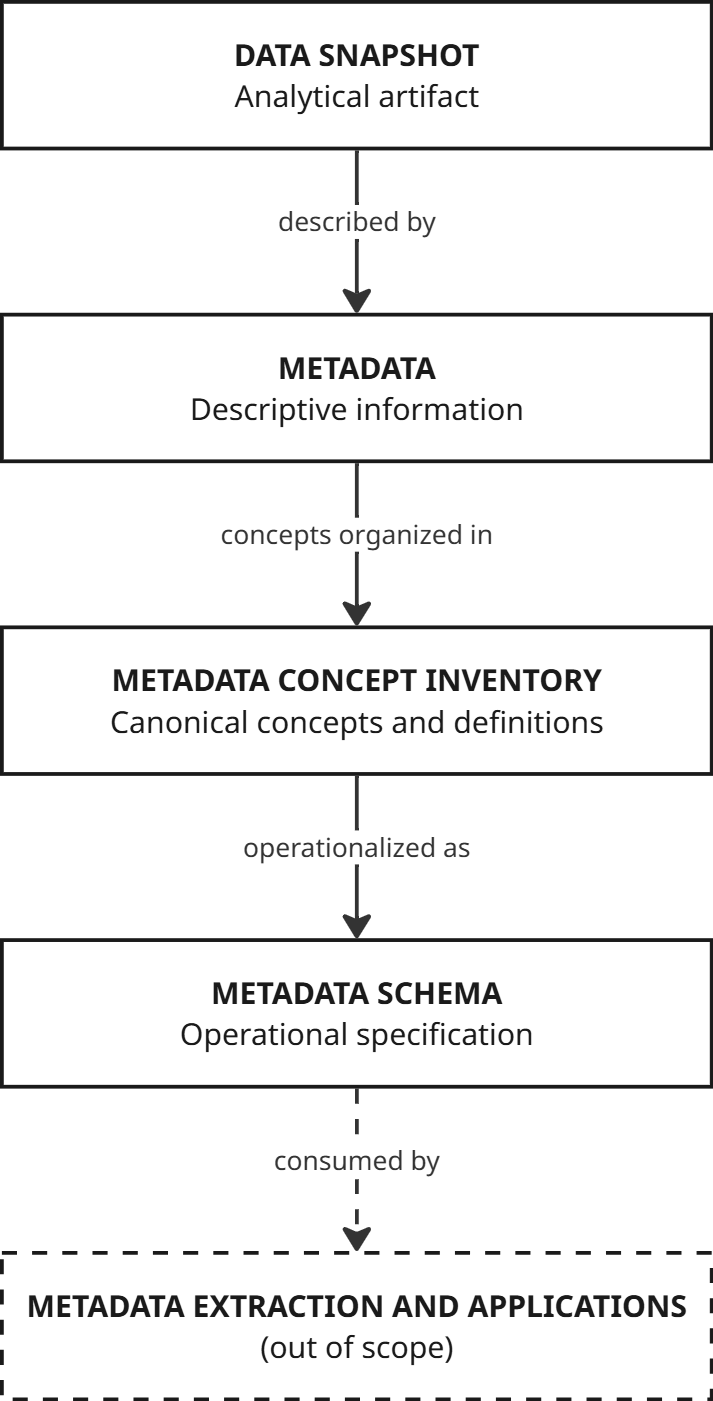
\includegraphics[width=0.95\linewidth]{data/conceptual_hierarchy.png}
    \caption{Relationship between data snapshots, metadata, the intermediate concept inventory, and the metadata schema. Metadata extraction and downstream applications are shown separately because they assume that an operational metadata schema already exists.}
    \label{fig:conceptual_relationship}
\end{figure}

\subsection{Scope}

The proposed methodology addresses the development of an operational metadata schema for a class of multimodal analytical artifacts that lacks a dedicated schema or directly adoptable metadata profile. Existing standards and vocabularies may still provide applicable terms. The task is to identify, consolidate, define, and operationalize descriptive requirements grounded in representative artifacts.

Schema design first produces an operational representation whose coverage is assessed against held-out artifacts. Standards-informed refinement then compares the validated schema with relevant standards and application-profile practices and incorporates human-approved changes that preserve the artifact-derived requirements. The endpoint of the methodology is therefore a standards-informed operational metadata schema accompanied by held-out validation evidence, a standards crosswalk, and a record of human adjudication decisions. Metadata extraction and downstream applications remain outside the scope of this work, as do subsequent activities that adapt the schema to a particular machine-readable implementation.

\subsection{Problem definition}

Schema development for established resource types can draw on mature standards, shared conventions, and accumulated domain knowledge. When an artifact class is not yet adequately characterized, its descriptive requirements cannot be assumed in advance. Defining fields solely from expert expectations or a small number of salient examples may omit less frequent properties that remain important for interpretation or discovery. The schema must therefore be grounded in evidence from representative artifacts before a shared vocabulary is fixed.

We therefore consider the following problem:

\begin{quote}
Given a representative collection of multimodal analytical artifacts for which no dedicated operational metadata schema exists, how can an operational metadata schema be systematically developed from artifact-level evidence?
\end{quote}

This problem presents five challenges. First, the relevant metadata space is initially unknown. Second, artifact-level observations are heterogeneous and local; they must be aggregated and consolidated while retaining traceability to their source artifacts. Third, the resulting concept inventory must be translated into fields, definitions, and guidance suitable for consistent use. Operational design must balance annotation consistency, retrieval utility, usability, and maintainability. Fourth, the completed schema must be evaluated on held-out artifacts without treating every rare semantic distinction as evidence for a new field. Finally, standards-informed refinement must improve terminology and representation without displacing requirements established from the artifacts themselves.

We address these challenges by decomposing metadata schema development into a sequence of evidence-preserving semantic transformations connected by explicit intermediate knowledge artifacts. LLMs support broad metadata discovery, semantic consolidation, structured gap analysis, and standards research, with multimodal capabilities used for image-based discovery and validation. Human experts retain responsibility for scope, conceptual boundaries, operational schema design, validation adjudication, and final standards-informed decisions.

\section{Methodology}
\label{sec:methodology}

This section presents a reusable methodology for developing an operational metadata schema for multimodal analytical artifacts that lack a dedicated schema or directly adoptable metadata profile. It decomposes schema development into a sequence of evidence-preserving semantic transformations connected by explicit intermediate knowledge artifacts. LLMs support selected discovery, consolidation, and assessment tasks, with multimodal capabilities used for image-based discovery and validation; human experts retain responsibility for conceptual and operational decisions.

The stages separate metadata discovery, field profile aggregation, canonical metadata concept synthesis, expert concept refinement, concept coverage assessment, metadata schema design and specification, schema validation, and standards-informed schema refinement. This decomposition makes each transformation independently reviewable and preserves traceability from the final operational schema to the artifacts and standards that informed it. Table~\ref{tab:methodology_summary} summarizes the workflow.

\begin{table}[!ht]
    \centering
    \caption{Summary of the proposed methodology. Each stage transforms an explicit input artifact into an output that can be reviewed before the next stage.}
    \label{tab:methodology_summary}
    \renewcommand{\arraystretch}{1.4}

    \newcolumntype{Y}[1]{>{\hsize=#1\hsize\raggedright\arraybackslash}X}

    \begin{tabularx}{\textwidth}{Y{0.9} Y{1.25} Y{0.9} Y{0.95}}
    \toprule

    \textbf{Workflow stage} &
    \textbf{Semantic transformation} &
    \textbf{Primary LLM contribution} &
    \textbf{Primary human contribution} \\

    \midrule

    Metadata discovery &
    Representative artifacts \newline $\downarrow$ \newline Metadata observations &
    Artifact interpretation and broad discovery &
    Sampling and discovery criteria \\

    \midrule

    Field profile aggregation &
    Metadata observations \newline $\downarrow$ \newline Metadata field profiles &
    -- &
    Aggregation design and quality review \\

    \midrule

    Canonical metadata concept synthesis &
    Metadata field profiles \newline $\downarrow$ \newline Candidate metadata concept inventory &
    Semantic consolidation and canonicalization &
    Synthesis criteria and prompt design \\

    \midrule

    Expert concept refinement &
    Candidate metadata concept inventory \newline $\downarrow$ \newline Refined metadata concept inventory &
    Decision support &
    Conceptual boundary and refinement decisions \\

    \midrule

    Concept coverage assessment &
    Refined metadata concept inventory and field profiles \newline $\downarrow$ \newline Concept coverage evidence &
    Constrained classification &
    Interpretation and further refinement \\

    \midrule

    Metadata schema design and specification &
    Refined metadata concept inventory \newline $\downarrow$ \newline Operational metadata schema &
    Design and documentation assistance &
    Operational representation decisions \\

    \midrule

    Schema validation &
    Operational metadata schema and held-out artifacts \newline $\downarrow$ \newline Validation evidence and justified revisions &
    Open gap discovery and confirmatory assessment &
    Gap adjudication and revision decisions \\

    \midrule

    Standards-informed schema refinement &
    Validated operational metadata schema and relevant standards \newline $\downarrow$ \newline Standards-informed operational metadata schema and decision record &
    Standards research, candidate mappings, and comparison &
    Acceptance, rejection, and deferral decisions \\

    \bottomrule
    \end{tabularx}
\end{table}

The methodology progressively transforms artifact-level observations into a shared concept inventory and then into an operational metadata schema. Held-out validation evaluates that schema and records justified revisions. Standards-informed refinement then compares the validated schema with relevant external terms and representation practices while preserving the artifact-derived requirements established by the preceding stages. The methodology is presented independently of the case study; implementation-specific details are deferred to Section~\ref{sec:case_study}.

\subsection{Metadata discovery}

The objective of metadata discovery is to identify candidate descriptive properties evidenced in representative analytical artifacts. This stage emphasizes discovery breadth rather than semantic precision and therefore retains potentially useful metadata observations even when they may later prove redundant, ambiguous, or outside the final schema's scope.

This stage begins with a representative sample of multimodal analytical artifacts drawn from the target domain. The methodology assumes that the sample captures the diversity of artifact types, reporting styles, and semantic content expected in downstream applications.

Each artifact is processed independently using a multimodal LLM, which proposes candidate metadata fields from the artifact's visual and textual content rather than selecting from a predefined vocabulary. Independent processing prevents early convergence toward a shared vocabulary and limits influence from previously processed artifacts. Redundancy and semantic overlap are therefore intentional: candidate fields may use synonymous terms, reflect different levels of abstraction, or represent concepts later excluded from the final schema.

Metadata observations are generated without human curation or filtering to preserve discovery breadth and reduce the risk of prematurely excluding useful concepts. Human involvement is therefore limited to defining the discovery objective, selecting representative artifacts, and designing the prompting strategy. The output of this stage is a collection of metadata observations describing the sampled artifacts. These observations serve as the input to field profile aggregation.

\subsection{Field profile aggregation}

Field profile aggregation consolidates the observations produced during metadata discovery into \emph{metadata field profiles}. Subsequent stages operate on these profiles rather than individual observations, reducing the context they must process and establishing the profiles as the primary units of semantic reasoning.

This stage groups metadata observations referring to the same candidate metadata field into a single metadata field profile using deterministic exact-name matching, without semantic normalization or canonicalization (e.g., "geographic location" and "geographic locations" remain separate profiles). Each profile aggregates representative supporting evidence—including frequent values, example descriptions, occurrence statistics, and explanatory reasoning—and provides a compact representation for subsequent concept synthesis.

The output of this stage is a collection of metadata field profiles that represent the unique candidate metadata fields identified across the representative artifact collection and serve as the input to canonical metadata concept synthesis.

\subsection{Canonical metadata concept synthesis}

Canonical metadata concept synthesis transforms the metadata field profiles into a \emph{candidate metadata concept inventory}. Whereas metadata discovery emphasizes broad semantic exploration, concept synthesis identifies shared concepts across profiles and reduces terminological redundancy.

Unlike field profile aggregation, which groups observations using exact field names, this stage consolidates profiles that represent the same underlying metadata concept. Distinct concepts, including infrequently occurring ones, are retained so that consolidation does not remove potentially important descriptive requirements.

To reduce incorrect semantic merges, concept synthesis favors under-consolidation over premature consolidation. Concepts that remain separate can still be merged during expert refinement, whereas distinctions removed at this stage may be difficult to recover. For example, simple plural variants such as "geographic location" and "geographic locations" would typically be consolidated, whereas the relationship between concepts such as "data type" and "format" may require human judgment.

An LLM synthesizes the candidate inventory from the aggregated field profiles. Each canonical metadata concept includes a definition, representative examples, and a rationale for the proposed consolidation. The resulting inventory is the first shared representation of the discovered metadata space and serves as the input to expert concept refinement.

\subsection{Expert concept refinement}

Expert concept refinement transforms the candidate metadata concept inventory into a refined inventory suitable for schema design. Whereas concept synthesis emphasizes semantic abstraction, expert refinement establishes conceptual boundaries, scope, and internal consistency, thereby finalizing the canonical metadata vocabulary.

Refinement proceeds through an iterative review in which candidate metadata concepts are evaluated individually and in relation to the inventory as a whole. Typical activities include merging semantically equivalent concepts, splitting concepts that capture multiple ideas, renaming concepts, excluding concepts outside the intended metadata scope, refining definitions and examples, and clarifying boundaries between related concepts.

These decisions are guided primarily by semantic reasoning rather than empirical frequency. The objective is not to minimize the number of concepts, but to produce an inventory that is conceptually distinct, internally consistent, and appropriate for the intended application. A recurring consideration is the distinction between descriptive metadata and analytical content. Candidate concepts that represent values to be extracted from an artifact, rather than metadata describing the artifact, are excluded. This establishes a clear boundary between metadata schema development and downstream metadata extraction.

Human judgment governs this stage. An LLM may propose alternative names, identify overlapping definitions, summarize differences between concepts, and suggest refinements. Final decisions concerning merges, exclusions, definitions, and organization remain with the human expert. The output is a refined metadata concept inventory with defined semantic boundaries that serves as the conceptual foundation for metadata schema design.

\subsection{Concept coverage assessment}

Concept coverage assessment evaluates how the refined metadata concept inventory represents the metadata field profiles produced during field profile aggregation. Using evidence from the development collection, it characterizes how the inventory organizes the discovered metadata space and supports human review and any further refinement before schema design.

The assessment assigns each metadata field profile to one of the concepts in the refined inventory through constrained classification. An LLM or another suitable classifier may perform this assignment. The resulting mappings support quantitative analysis across the representative collection.

The concept assignments support analyses of concept frequency, corpus coverage, artifact-type coverage, rare concepts, and concepts receiving unexpectedly high or low empirical support. These analyses provide evidence rather than prescribing changes. Infrequent concepts, for example, may remain operationally important when they capture distinct aspects of the artifact class. Human interpretation of the coverage evidence may motivate further concept refinement before schema design. The output comprises concept assignments, descriptive statistics, and related analyses characterizing the coverage of the refined inventory.

\subsection{Optional extension: Scaling expert concept refinement}

Expert concept refinement relies primarily on human review. While this is practical for moderately sized inventories, exhaustive manual inspection becomes increasingly difficult as the number of concepts grows. For larger inventories, similarity-based analyses can provide optional decision support.

Similarity-based analyses identify relationships between metadata field profiles or canonical concepts using semantic similarity or co-occurrence. These relationships may be explored through hierarchical clustering, community detection, or network visualization to identify groups of closely related concepts.

These analyses support human judgment by highlighting candidate merges, unexpected clusters, isolated concepts, or parts of the inventory requiring additional inspection. They provide complementary evidence for expert refinement but do not replace semantic reasoning or automate conceptual decisions.

Accordingly, similarity-based analyses are optional decision-support mechanisms rather than mandatory workflow stages. Their value increases with inventory size and complexity by focusing human review on areas most likely to benefit from further inspection.

\subsection{Metadata schema design and specification}

Metadata schema design and specification transforms the refined metadata concept inventory into an operational metadata schema. Whereas concept refinement establishes a coherent representation of the metadata space, this stage determines how to represent the concepts as fields suitable for annotation, storage, retrieval, and downstream metadata extraction.

Design proceeds iteratively. Typical activities include representing conceptually distinct concepts within a single field when operationally appropriate, introducing fields required for practical use, excluding concepts whose implementation cost outweighs their operational value, refining field names and definitions, organizing fields into coherent modules, and developing annotation guidance, examples, and scope notes.

Concept refinement establishes \emph{which metadata concepts are relevant}; schema design determines \emph{how those concepts should be represented operationally}. The design therefore balances semantic distinctions with annotation consistency, usability, and maintainability. These trade-offs cannot be resolved through semantic reasoning alone. Conceptually distinct concepts may be represented by one field to simplify annotation, while an infrequent concept may be retained because it has clear operational value.

Human judgment governs schema design. An LLM may propose organizational structures, identify ambiguous definitions, suggest simplifications, and assist with annotation guidance. Final decisions concerning fields, constraints, organization, and documentation remain with the human expert.

The output is an operational metadata schema comprising fields, definitions, organization, annotation guidance, examples, and other documentation required for consistent metadata creation and downstream use.

\subsection{Schema validation}
\label{sec:schema_validation_methodology}

Schema validation evaluates the operational metadata schema against artifacts not used during its initial development. Unlike concept coverage assessment, which examines the refined concept inventory against field profiles from the development collection, schema validation occurs after schema design and tests the operational fields, definitions, and scope against held-out evidence.

Schema validation may combine complementary forms of assessment. Open residual discovery generates metadata observations from held-out artifacts and identifies observations that do not fit the schema well. Confirmatory coverage assessment examines each held-out artifact for metadata that is important to interpretation or discovery but lacks an adequate schema field. Together, these assessments test both broad residual coverage and consequential omissions.

Candidate gaps are not treated as automatic schema changes. Human experts review the supporting artifact evidence and determine whether each candidate represents a missing field, a documentation gap, a representation gap, an instance-specific detail, or an out-of-scope concept. Accepted findings may lead to schema revisions, after which the affected definitions or fields can be reassessed.

The output of this stage is a body of validation evidence, a record of human adjudication decisions, and any justified revisions to the operational metadata schema. These outputs support bounded conclusions about schema adequacy for the tested artifact collection and intended application; they do not establish universal coverage.

\subsection{Standards-informed schema refinement}
\label{sec:standards_refinement_methodology}

Standards-informed schema refinement compares the validated operational metadata schema with relevant metadata standards, domain vocabularies, and application-profile practices. This stage occurs after held-out validation so that external terminology and representation patterns refine an artifact-derived schema rather than determining its initial descriptive requirements.

The review begins by identifying standards relevant to the schema's descriptive scope. Each validated field is then compared with candidate external terms and classified according to whether the relationship is exact, close, broader, narrower, structural, or absent. The crosswalk may identify clearer definitions, more familiar terminology, applicable formats or controlled vocabularies, and representation patterns that distinguish concepts combined in the operational schema.

A standards mapping is not treated as an automatic schema change. Candidate refinements are evaluated against the artifact evidence, the intended application, and operational criteria including annotation consistency, retrieval utility, usability, and maintainability. Human reviewers accept changes that improve semantic accuracy without reducing coverage, reject mappings that narrow or distort the observed concepts, and defer structures that are valuable but unnecessary for the selected operational representation. Proposed mappings may be refined and reviewed iteratively before a decision is finalized.

LLM assistance may support standards discovery, comparison, and candidate mapping across multiple vocabularies. Human reviewers verify the sources and retain authority over field names, definitions, organization, cardinality, value guidance, and the treatment of unmatched local concepts. The output is a standards-informed operational metadata schema together with a crosswalk and decision record. This outcome is an application-specific specification; it does not constitute community standardization or evidence of interoperability performance.

\section{Case study: Developing the Data Snapshot Metadata Schema}
\label{sec:case_study}

This section applies the proposed methodology to develop the Data Snapshot Metadata Schema. It describes the artifact class, dataset, workflow execution, initial schema design, two complementary schema-validation exercises, and standards-informed refinement. The intermediate knowledge artifacts, validation evidence, and standards crosswalk provide the empirical basis for the subsequent analysis.

\subsection{Artifact type}

The case study focuses on \emph{data snapshots}: semantically meaningful analytical artifacts extracted from institutional PDF documents and managed as independent information objects. Data snapshots preserve their analytical meaning outside the context of their source documents and therefore require metadata describing the snapshot itself rather than only its source document.

Typical data snapshots include statistical tables, analytical charts, geospatial maps, monitoring dashboards, financial summaries, composite figures, and other visual analytical objects containing textual, numerical, and spatial information. Additional examples of data snapshots are provided in Appendix~\ref{appendix:datasnapshots}.

Prior work treats data snapshots as independent information objects to support retrieval, indexing, comparison, and metadata extraction at the level of the analytical artifact~\citep{dy2026}. At the outset of this study, no directly adoptable metadata schema had been identified for data snapshots as defined here. This made them an appropriate case for artifact-driven metadata schema development.

\subsection{Case study dataset}

Representative data snapshots were sampled from three institutional document corpora introduced in \cite{dy2026}, spanning humanitarian reporting, academic policy research, and development project operations. The corpora differ substantially in document structure, visualization conventions, and reporting style, providing a diverse collection of analytical artifacts for metadata discovery.

Within these corpora, data snapshots were extracted from document layout regions classified as either figures or tables. To ensure balanced coverage, sampling was stratified by corpus and artifact category, as summarized in Table~\ref{tab:composition}. Equal representation of figures and tables reduced bias toward the structural characteristics of either visualization type.

Although the dataset is not intended to be statistically representative of institutional documents as a whole, it provides semantic diversity across multiple reporting domains and visualization types for one execution of the proposed methodology.

\begin{table}[!ht]
    \centering
    \caption{Composition of the case study dataset.}
    \label{tab:composition}
    \begin{tabular}{lrrr}
        \toprule
        \textbf{Corpus} & \textbf{Figures} & \textbf{Tables} & \textbf{Total} \\
        \midrule
        UNHCR / ReliefWeb & 35 & 35 & 70 \\
        Policy Research Working Papers & 35 & 35 & 70 \\
        Refugee Project Appraisal Documents & 35 & 35 & 70 \\
        \midrule
        \textbf{Total} & \textbf{105} & \textbf{105} & \textbf{210} \\
        \bottomrule
    \end{tabular}
\end{table}

\subsection{Workflow execution}

We executed the development stages using the 210-snapshot case study dataset. Metadata discovery processed each snapshot independently; subsequent stages aggregated the observations, synthesized and refined a shared concept inventory, assessed concept coverage, and translated the refined inventory into an operational metadata schema. The schema was then evaluated against held-out snapshots and refined through comparison with relevant standards. Figure~\ref{fig:artifact_evolution} shows the intermediate knowledge artifacts produced during this process.

Metadata discovery and canonical metadata concept synthesis used GPT-5.5, while concept coverage assessment used GPT-5.4 mini for constrained classification. Field profile aggregation was implemented deterministically in Python and required no LLM inference. Expert concept refinement and metadata schema design and specification were performed through iterative human review of the intermediate knowledge artifacts. Model configurations and implementation summaries for these stages are provided in Appendices~\ref{appendix:discovery}--\ref{appendix:validation}; the complete prompts, structured-output definitions, and executable implementations are available in the accompanying repository.

\begin{figure}[!ht]
    \centering
    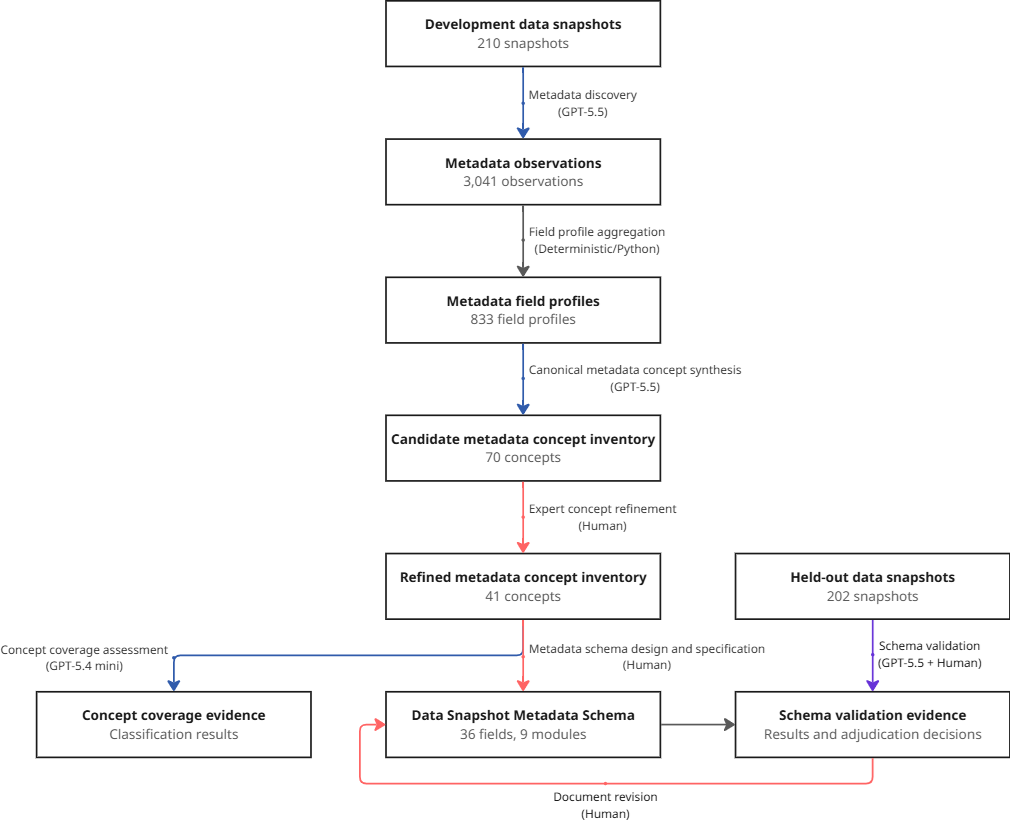
\includegraphics[width=0.95\textwidth]{data/case_study_execution.png}
    \caption{Case-study execution of the proposed methodology. The workflow transforms 210 development snapshots into an initial 36-field schema, with schema validation performed on a separate collection of 202 held-out snapshots. Human revision produces the validated 36-field schema, which is then refined against authoritative standards and vocabularies to produce the final 37-field Data Snapshot Metadata Schema. Colors distinguish LLM-supported, deterministic, human-guided, and joint LLM–human transformations.}
    \label{fig:artifact_evolution}
\end{figure}

\subsection{Initial metadata schema}

Metadata schema design produced an initial operational Data Snapshot Metadata Schema comprising 36 metadata fields organized into nine semantic modules. The schema translated the refined metadata concept inventory into fields, definitions, and annotation guidance for subsequent metadata workflows.

A central design decision was the separation of metadata describing the snapshot from analytical content to be extracted from it. This boundary kept the metadata record focused on the identity, interpretation, organization, and management of the snapshot rather than reproducing all values contained in the artifact.

\subsection{Schema validation}
\label{sec:schema_validation_case_study}

A separate collection of 202 snapshots was held out from metadata discovery through initial schema design and used only for held-out schema validation. It contained up to 35 figures and 35 tables from each corpus; only 27 eligible figures remained in the Refugee Project Appraisal Document corpus after the 210 case study snapshots were excluded (Table~\ref{tab:validation_composition}). Both validation exercises used this same held-out collection and addressed different questions using the same evidence.

\begin{table}[!ht]
    \centering
    \caption{Held-out collection used in both schema-validation exercises.}
    \label{tab:validation_composition}
    \begin{tabular}{lrrr}
        \toprule
        \textbf{Corpus} & \textbf{Figures} & \textbf{Tables} & \textbf{Total} \\
        \midrule
        UNHCR / ReliefWeb & 35 & 35 & 70 \\
        Policy Research Working Papers & 35 & 35 & 70 \\
        Refugee Project Appraisal Documents & 27 & 35 & 62 \\
        \midrule
        \textbf{Total} & \textbf{97} & \textbf{105} & \textbf{202} \\
        \bottomrule
    \end{tabular}
\end{table}

Validation 1 used open residual discovery to test the frozen Data Snapshot Metadata Schema. It produced 2,876 evidence-bearing metadata observations, of which 2,275 (79.1\%) were classified as covered by an existing field. Weak-fit and no-fit observations produced 578 candidate-field proposals. Human review consolidated related names, inspected the supporting evidence, and accepted no candidate as a new field. The review instead identified documentation ambiguities and limitations in how the flat schema represented several existing concepts. The resulting documentation revision clarified definitions and scope without changing the 36-field inventory.

Validation 2 used a confirmatory assessment to test whether the documentation-revised Data Snapshot Metadata Schema omitted metadata that was critical to interpreting or discovering each held-out snapshot. The model assessed 197 snapshots (97.5\%) as having no critical gap, five (2.5\%) as having a possible gap, and none as having a critical gap. The five positive snapshots produced six possible-gap records. Human review accepted no new field: four candidates were rejected or excluded, while two exposed representation limitations involving panel-level metadata and nested table-column structure.

Table~\ref{tab:schema_validation_results} summarizes the two exercises.

\begin{table}[!ht]
    \centering
    \caption{Summary of the two schema-validation exercises. Both used the same 202 snapshots held out from metadata discovery through initial schema design.}
    \label{tab:schema_validation_results}
    \renewcommand{\arraystretch}{1.4}

    \newcolumntype{Y}[1]{>{\hsize=#1\hsize\raggedright\arraybackslash}X}

    \begin{tabularx}{\textwidth}{Y{0.7} Y{1.15} Y{1.15}}
    \toprule

    \textbf{Measure} & \textbf{Validation 1} & \textbf{Validation 2} \\
    \midrule

    Assessment mode & Open residual discovery & Confirmatory critical-gap assessment \\
    Primary unit of assessment & Metadata observation & Data snapshot \\
    Held-out snapshots & 202 & 202 \\
    Main model output & 2,876 observations\newline 578 candidate-field proposals & 197 snapshots with no critical gap\newline 5 possible-gap snapshots\newline 6 possible-gap records \\
    Accepted new fields after human review & 0 & 0 \\

    \bottomrule
    \end{tabularx}
\end{table}

Because both exercises used the same held-out collection, they provide complementary evidence rather than independent replications. Validation 1 tested whether broad residual discovery would reveal additional field candidates; Validation 2 tested whether any remaining omission materially affected interpretation or discovery. After human adjudication, neither exercise identified a candidate that would have changed the accepted 36-field inventory. This result supports the adequacy of the inventory for the intended schema scope and tested collections, but does not establish universal coverage of all future data snapshots.

Model configurations and human-adjudication procedures for both exercises are documented in Appendix~\ref{appendix:schema_validation}; the complete prompts, structured-output definitions, and executable implementations are available in the accompanying repository.

\subsection{Standards-informed schema refinement}
\label{sec:standards_refinement_case_study}

Following schema validation, the 36 fields were compared with authoritative sources grouped by their role in the crosswalk. General metadata and catalog vocabularies included DCMI Metadata Terms, Schema.org, and DCAT 3~\citep{dcmi2020terms,schemaorg2026,albertoni2024dcat3}. Statistical and research-data references included SDMX 3.1 and DDI Lifecycle 3.3~\citep{sdmx2025standards,ddi2020lifecycle33}. Provenance, publishing, controlled-vocabulary, and project-finance sources included PROV-O, JATS 1.3, SKOS, and IATI 2.03~\citep{lebo2013provo,niso2021jats13,miles2009skos,iati203}, together with applicable value and format standards.

OpenAI Codex software supported standards discovery, comparison, and draft mappings using the validated schema, the validation findings, and authoritative standards documentation. For each schema field, the review classified the relationship to candidate external terms as exact, close, broader, narrower, related or structural, or having no direct match. Candidate refinements could concern field terminology, definitions, semantic boundaries, value guidance, or representation structure.

Human review treated the crosswalk as evidence for schema refinement rather than as an automatic substitution rule. Proposed mappings and refinements were assessed against the artifact evidence, validation findings, intended application, and the requirement that the paper specification remain directly inspectable. Changes were accepted when they improved semantic accuracy without reducing coverage, rejected when they narrowed or distorted observed concepts, and deferred when they required richer relational or machine-enforceable structures beyond the flat specification used in this study. Appendix~\ref{appendix:standards_refinement} documents the sources, review configuration, and procedure.

\subsection{Resulting metadata schema}

Standards-informed refinement produced the final Data Snapshot Metadata Schema with 37 fields organized into the same nine semantic modules (Table~\ref{tab:schema}). The additional field resulted from separating derivation sources from attributions; it did not represent a metadata omission discovered after validation. The final specification preserves the information coverage established by the artifact-driven and validation stages while adopting terminology, semantic distinctions, and guidance supported by the standards review.

\begin{table}[!ht]
    \centering
    \caption{Semantic organization of the standards-informed Data Snapshot Metadata Schema.}
    \label{tab:schema}
    \small
    \begin{tabular}{llr}
        \toprule
        \textbf{Semantic module} & \textbf{Representative fields} & \textbf{Fields} \\
        \midrule
        Identity \& Discovery & \makecell[l]{\texttt{title} \\ \texttt{document\_label} \\ \texttt{subject\_domains}} & 5 \\
        \midrule
        Subject \& Semantics & \makecell[l]{\texttt{variable\_names} \\ \texttt{population\_group}} & 4 \\
        \midrule
        Temporal Context & \makecell[l]{\texttt{time\_period} \\ \texttt{temporal\_granularity}} & 2 \\
        \midrule
        Spatial Context & \makecell[l]{\texttt{geographic\_scope} \\ \texttt{geographic\_entities}} & 5 \\
        \midrule
        Measurement Context & \makecell[l]{\texttt{units\_of\_measure} \\ \texttt{statistical\_forms}} & 4 \\
        \midrule
        Structural Organization & \makecell[l]{\texttt{row\_dimensions} \\ \texttt{visualization\_types}} & 3 \\
        \midrule
        Provenance \& Attribution & \makecell[l]{\texttt{data\_sources} \\ \texttt{attributions} \\ \texttt{languages}} & 5 \\
        \midrule
        Project \& Operational Context & \makecell[l]{\texttt{project\_name} \\ \texttt{financing\_measures} \\ \texttt{funders}} & 7 \\
        \midrule
        Analytical \& Methodological Context & \makecell[l]{\texttt{analysis\_methods} \\ \texttt{data\_collection\_methods}} & 2 \\
        \midrule
        \textbf{Total} & & \textbf{37} \\
        \bottomrule
    \end{tabular}
\end{table}

Appendix~\ref{appendix:schema} reproduces the complete reference specification, and Appendix~\ref{appendix:sample_metadata} provides three data snapshots with sample metadata records.

The resulting schema, intermediate knowledge artifacts, held-out validation evidence, standards crosswalk, and human decision record document one complete execution of the methodology. The following section examines the contribution of each semantic transformation.

\section{Analysis of evidence-preserving semantic transformations}

The case study produced a sequence of explicit artifacts: metadata observations, metadata field profiles, candidate and refined metadata concept inventories, concept coverage evidence, an initial operational metadata schema, held-out validation evidence, a standards crosswalk and decision record, and the final standards-informed schema. Together, they document the transformation of artifact-level evidence into an operational specification, the evaluation of that specification, and its refinement against relevant standards.

This section examines how the intermediate knowledge artifacts reduced semantic complexity, preserved supporting evidence, and structured the respective contributions of the LLM and human expert. It then considers what the held-out validation and standards review contributed to the resulting schema.

The analysis is organized around seven questions:

\begin{enumerate}
    \item How did independent metadata discovery characterize the semantic space?
    \item How did metadata field profile aggregation transform localized observations into reusable semantic evidence?
    \item How did concept synthesis and expert refinement transform semantic evidence into a coherent concept inventory?
    \item How did concept coverage assessment characterize the refined inventory?
    \item How did metadata schema design transform the concept inventory into an operational specification?
    \item What did held-out schema validation show about the accepted field inventory?
    \item How did standards-informed refinement change the validated schema?
\end{enumerate}

\subsection{Independent semantic discovery}

Independent metadata discovery first characterized the semantic space of the target artifact type. Each development snapshot was analyzed separately, allowing candidate descriptions to emerge without influence from a vocabulary established from previously processed snapshots. This design prioritized artifact-level evidence before vocabulary normalization or concept consolidation.

Metadata discovery produced 3,041 metadata observations representing candidate metadata fields across the 210 development snapshots (Table~\ref{tab:discovery_productivity}). Consistent with the prompting objective of identifying 10--15 reusable metadata fields per artifact, each snapshot yielded approximately 14--15 candidate metadata fields. The narrow distribution shows that the number of proposed fields remained tightly concentrated around this target across visualization types and document collections.

At this stage, multimodal reasoning combined textual, visual, and structural evidence. Rather than extracting values for predefined fields, the model proposed descriptive dimensions supported by titles, labels, legends, table structure, visual encodings, and the supplied document context. The outputs remained candidate observations whose relevance and scope were evaluated in later transformations.

\begin{table}[!ht]
    \centering
    \caption{Summary statistics for metadata discovery.}
    \label{tab:discovery_productivity}
    \begin{tabular}{lr}
        Number of snapshots & 210 \\
        Number of metadata observations & 3,041 \\
        Mean observations per snapshot & 14.48 \\
        \quad Median & 15 \\
        \quad Std dev & 0.89 \\
        \quad Min & 10 \\
        \quad Max & 16 \\
    \end{tabular}
\end{table}

The 3,041 observations corresponded to 833 unique candidate metadata fields after grouping identical field names, revealing a large candidate vocabulary. The discovered vocabulary exhibited a strongly skewed frequency distribution: approximately half of all observations belonged to only the 20 most frequently proposed metadata fields, while the remaining observations formed a long tail of increasingly specialized or infrequently proposed vocabulary (Figure~\ref{fig:topk_coverage}). Conversely, 581 candidate metadata fields appeared only once across the entire dataset.

\begin{figure}[!ht]
\centering
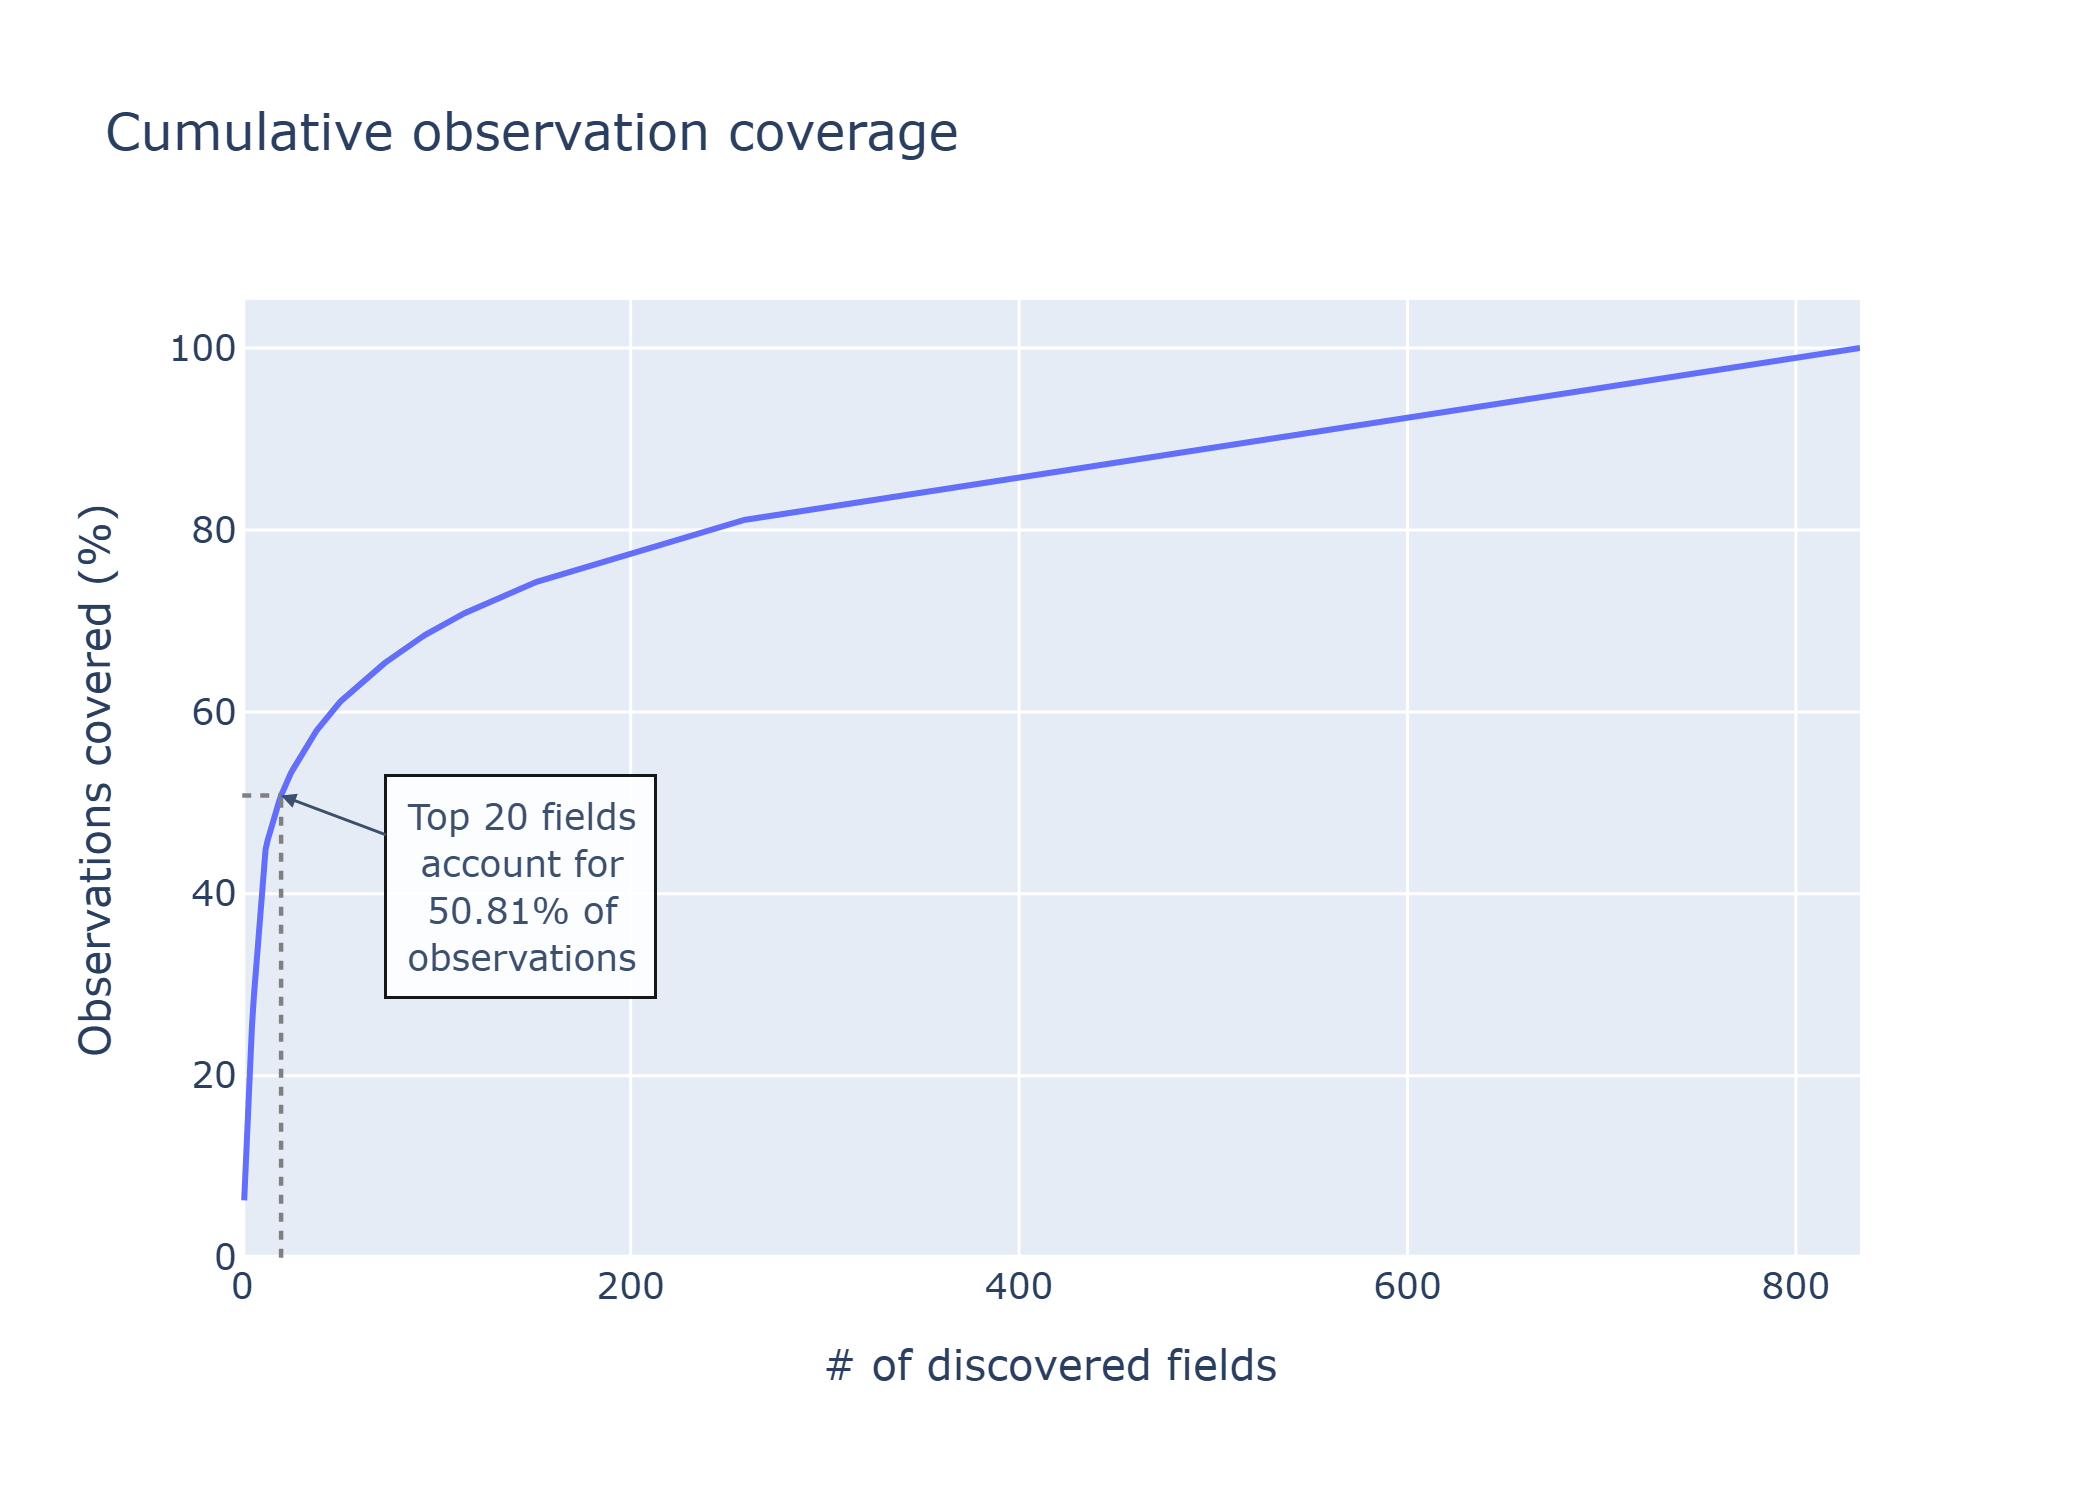
\includegraphics[width=0.75\linewidth]{data/topk_coverage.png}
\caption{Cumulative observation coverage as additional discovered metadata fields are included in descending order of frequency. The top 20 most frequently proposed metadata fields cover half of all observations.}
\label{fig:topk_coverage}
\end{figure}

Inspection of these singleton fields revealed that much of the apparent diversity arose from lexical variation rather than fundamentally different semantics. Semantically related concepts frequently appeared under different names, levels of abstraction, or contextual interpretations, including variations in aggregation terminology, administrative boundary descriptions, and indicator naming conventions. Consequently, the long tail reflects both genuine semantic diversity and the absence of early vocabulary normalization.

The discovered vocabulary also continued to expand throughout the development collection (Figure~\ref{fig:vocabulary_growth}). Even after all 210 development snapshots had been analyzed, each additional snapshot introduced an average of approximately four previously unseen candidate metadata fields. Repeated random shuffling of the dataset produced nearly identical accumulation curves, indicating that the continued growth was not an artifact of processing order.

Within the development collection, the discovered vocabulary continued to expand without evidence of saturation. This pattern did not establish that each new field name represented a new metadata requirement. Instead, it showed why the accumulated observations required a subsequent transformation that could distinguish lexical variation from meaningful conceptual distinctions.

\begin{figure}[t]
\centering
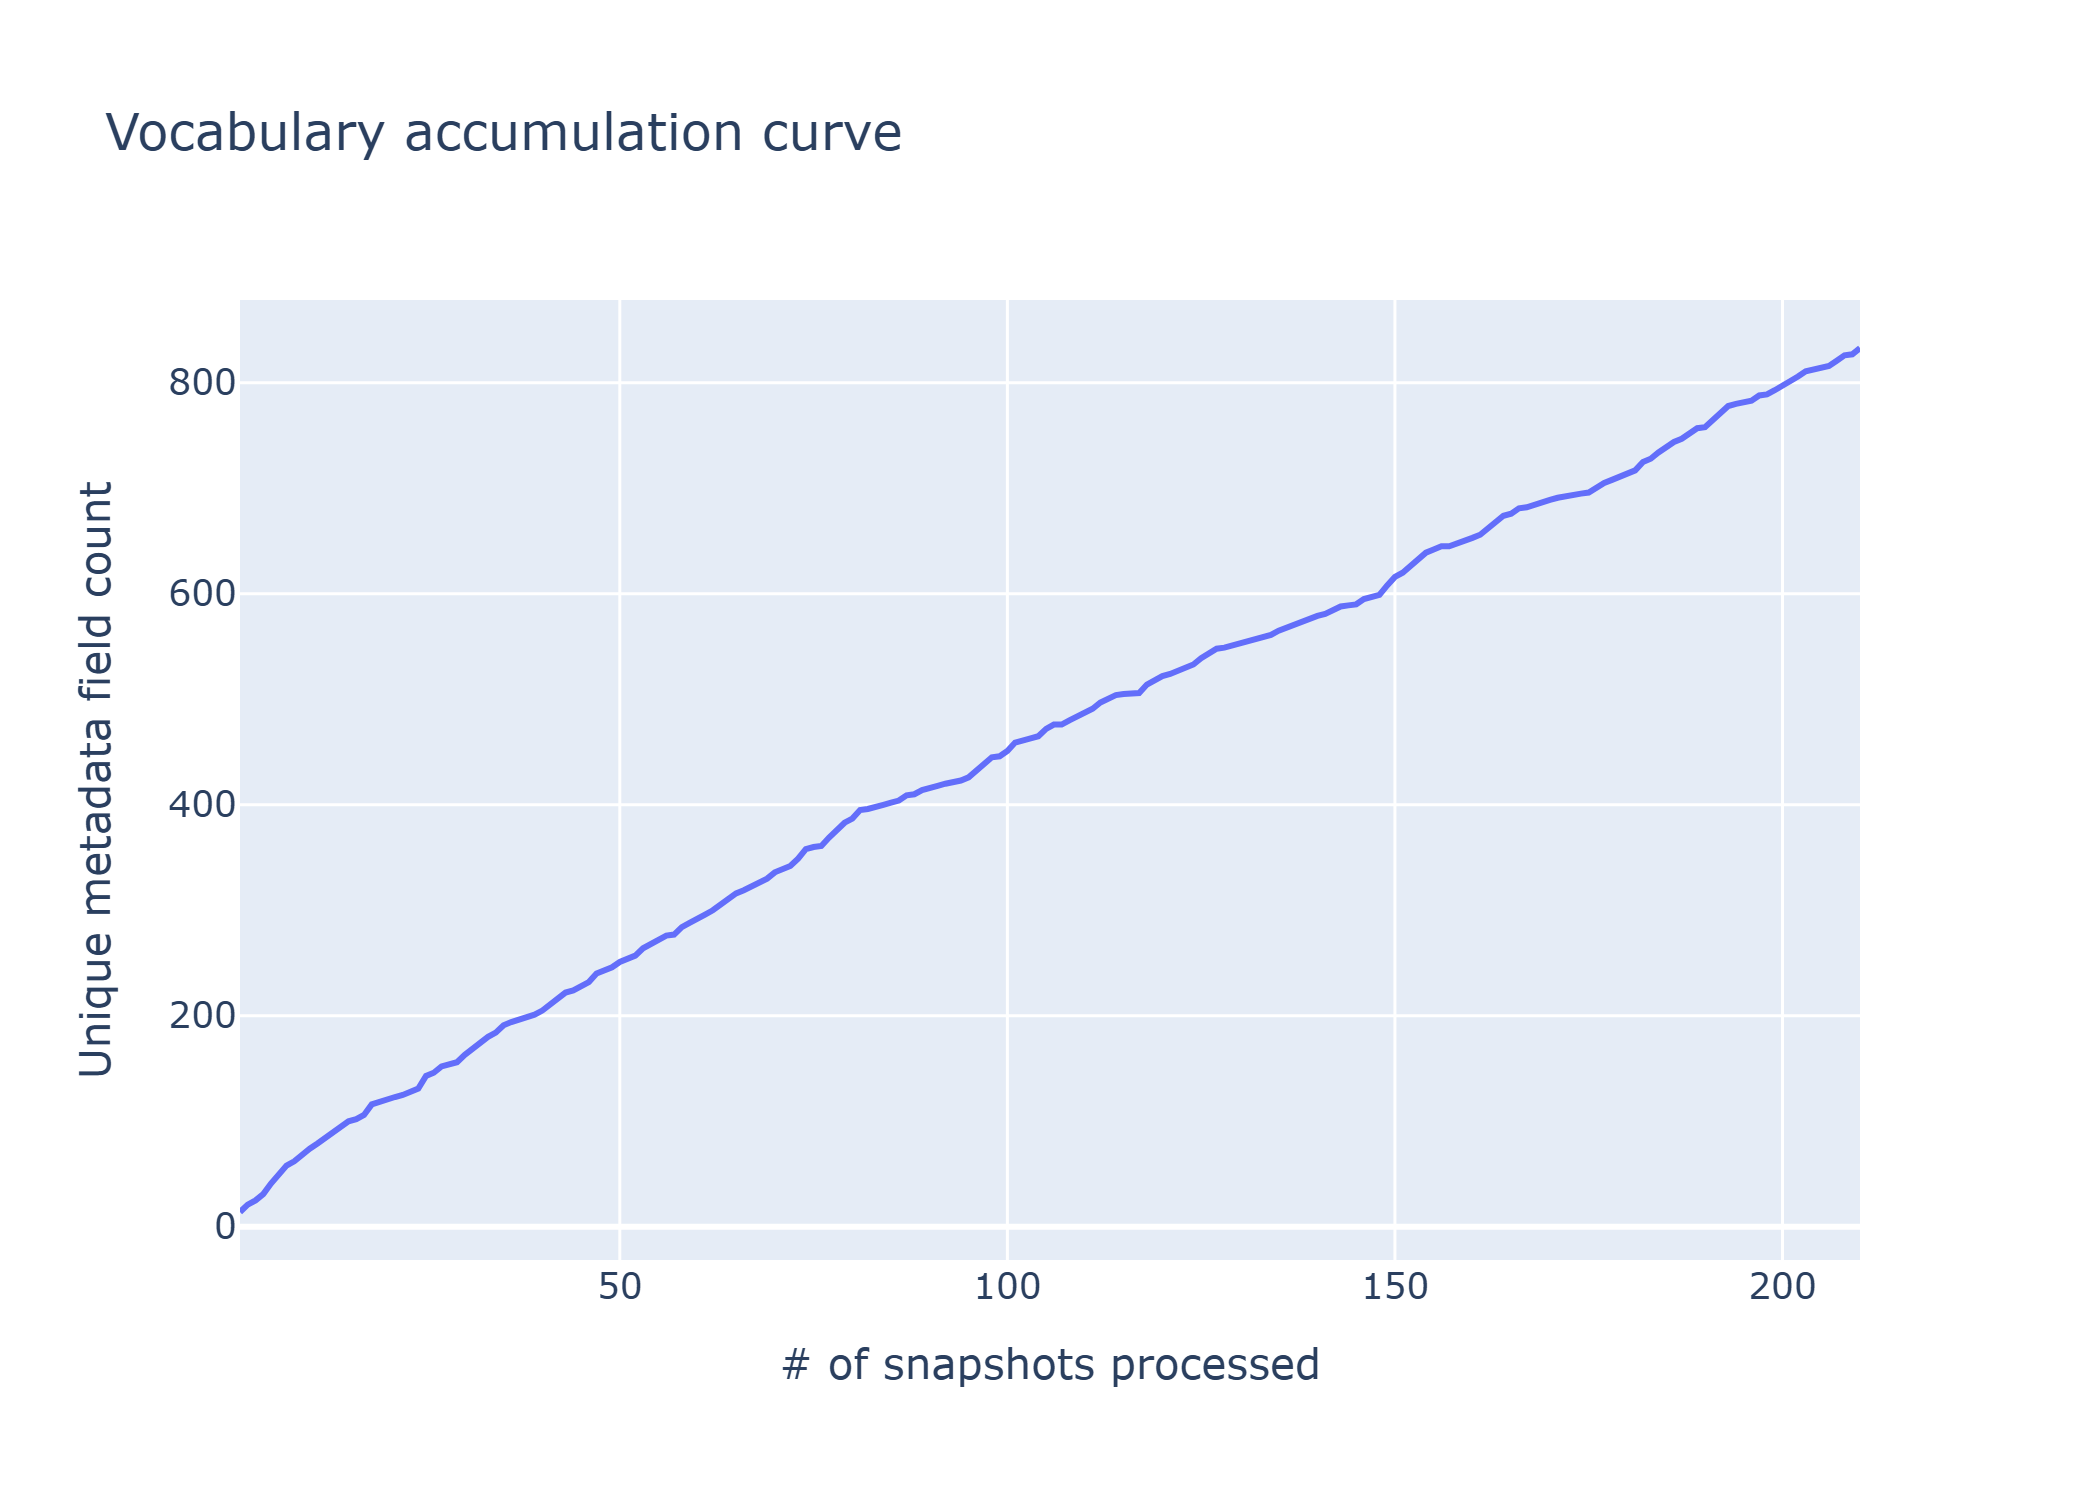
\includegraphics[width=0.75\linewidth]{data/vocabulary_growth.png}
\caption{Vocabulary accumulation curve showing the cumulative number of unique candidate metadata fields discovered as additional data snapshots were processed.}
\label{fig:vocabulary_growth}
\end{figure}

Taken together, these observations characterize independent metadata discovery as an exploratory stage of metadata schema development. Across the development collection, the process consistently identified candidate metadata while exposing a large and continually expanding vocabulary. Retaining the local descriptions, values, and rationales preserved artifact-level evidence that an immediately updated shared schema would not retain as separate records. That evidence provided the basis for distinguishing lexical variants from substantively different concepts during later synthesis.

\subsection{Metadata field profiles as reusable semantic evidence}

Metadata discovery produces localized observations that preserve semantic diversity but are too numerous and fragmented for direct expert comparison. Metadata field profiles bridge this gap by aggregating observations that share the same candidate field into a single evidence-bearing representation.

Aggregating the 3,041 metadata observations resulted in 833 metadata field profiles, reducing the number of semantic units requiring subsequent analysis by approximately 73\% (Table~\ref{tab:aggregation_summary}). This operation performed no semantic abstraction: it combined repeated occurrences of identical candidate metadata fields while preserving representative observed values, descriptive summaries, explanatory reasoning, and occurrence statistics.

\begin{table}[!ht]
    \centering
    \caption{Effect of metadata field profile aggregation.}
    \label{tab:aggregation_summary}
    \begin{tabular}{lr}
        Number of metadata observations & 3,041 \\
        Number of metadata field profiles & 833 \\
        Reduction & 72.6\% \\
    \end{tabular}
\end{table}

The principal effect of aggregation was not compression alone, but a change in the unit of semantic reasoning. Each metadata observation represents a localized interpretation of one artifact. A metadata field profile instead summarizes the collective evidence associated with a candidate field across the development collection. Concept synthesis therefore operates on evidence-bearing profiles rather than thousands of isolated observations.

This change enriches the evidence available for conceptual abstraction. Individual observations contain evidence from one artifact. Metadata field profiles accumulate representative values, descriptive summaries, rationales, occurrence statistics, and empirical support across multiple artifacts. Concept synthesis can therefore compare candidate fields using their accumulated semantic characteristics rather than their names alone.

\begin{table}[!ht]
    \centering
    \caption{Illustrative metadata field profile generated through aggregation. Each profile consolidates metadata observations sharing the same candidate metadata field into a reusable semantic evidence unit.}
    \label{tab:field_profile_example}
    \renewcommand{\arraystretch}{1.4}
    \newcolumntype{Y}[1]{>{\hsize=#1\hsize\raggedright\arraybackslash}X}
    \begin{tabularx}{\textwidth}{Y{0.6} Y{1.4}}
    \toprule
    
    \textbf{Metadata field profile component} & \textbf{Example content} \\
    \midrule
    
    Candidate metadata field & \texttt{geographic\_scope} \\
    
    Occurrence count & 192 metadata observations \\
    
    Representative values & Lebanon, Djibouti, Uganda, Croatia, World \\
    
    Representative descriptions &
    • Country or geographic area to which the table applies.\newline
    • Broad geographic region covered by the visualization. \\
    
    Representative reasoning &
    • Enables country-level search, filtering, and comparison.\newline
    • Provides geographic context for retrieval. \\

    Corpora represented & 3 corpora \\
    
    Artifact distribution & 96 figures, 96 tables \\

    \bottomrule
    \end{tabularx}
\end{table}

Inspection of representative field profiles (Table~\ref{tab:field_profile_example}) illustrates the value of this richer representation. Frequently occurring metadata fields accumulated diverse values, semantic descriptions, explanatory rationale, occurrence statistics, and provenance across many artifacts, while less common fields likewise retained sufficient contextual evidence for semantic interpretation.

Metadata field profiles therefore do more than reduce the number of semantic units requiring analysis. They transform localized observations into reusable semantic evidence while preserving the diversity discovered during the previous stage. This intermediate knowledge artifact connects independent discovery to shared concept synthesis and makes each later concept traceable to supporting observations. Metadata field profiles emerged during implementation rather than being specified in the initial workflow design, illustrating how an intermediate knowledge artifact can clarify the reasoning required between two transformations.

\subsection{Progressive concept synthesis and expert refinement}

Metadata field profiles preserve rich semantic evidence but remain too numerous for direct expert review. Two complementary stages transformed the 833 profiles into a coherent metadata concept inventory: conservative LLM-assisted concept synthesis followed by iterative expert refinement. This separation assigned semantic consolidation and final conceptual decisions to distinct stages (Table~\ref{tab:ontology_progression}).

\begin{table}[!ht]
    \centering
    \caption{Progressive reduction in semantic units during concept synthesis and expert refinement.}
    \label{tab:ontology_progression}
    \begin{tabular}{lr}
    \toprule
        \textbf{Stage} & \textbf{Semantic units} \\
        \midrule
        Metadata field profiles & 833 \\
        Candidate metadata concept inventory & 70 \\
        Refined metadata concept inventory & 41 \\
    \bottomrule
    \end{tabular}
\end{table}

Canonical metadata concept synthesis consolidated the discovered semantic space by grouping metadata field profiles that represented the same underlying concept despite differences in terminology, disciplinary perspective, or level of abstraction. Rather than maximizing semantic compression, the LLM was instructed to merge conservatively and retain plausible distinctions when uncertainty remained. This reduced 833 field profiles to a candidate inventory of 70 concepts intended to apply across the reporting domains represented in the case study. The reduction made the evidence more tractable for expert review while preserving distinctions that required human adjudication. Expert refinement then transformed the candidate inventory into a refined inventory of 41 concepts through recurring decisions to merge, rename, or exclude concepts (Table~\ref{tab:ontology_decisions}).

\begin{table}[!ht]
    \centering
    \caption{Representative expert concept-refinement decisions.}
    \label{tab:ontology_decisions}
    \renewcommand{\arraystretch}{1.4}
    \newcolumntype{Y}[1]{>{\hsize=#1\hsize\RaggedRight\arraybackslash}X}
    \renewcommand{\tabularxcolumn}[1]{m{#1}}
    
    \begin{tabularx}{\textwidth}{Y{0.4} Y{1.15} Y{1.45}}
    \toprule
        \textbf{Decision} & \textbf{Representative examples} & \textbf{Rationale} \\
        \midrule
        Concept merge &
          \texttt{measure\_name} \newline \quad $\rightarrow$ \texttt{indicator\_name} \newline
          \texttt{axis\_variable} \newline \quad $\rightarrow$ \texttt{indicator\_name} \newline
          \texttt{outcome\_variable} \newline \quad $\rightarrow$ \texttt{indicator\_name} &
          These are equivalent analytical variables expressed using different visualization or disciplinary terminology. \\
        \midrule
        Concept rename &
          \texttt{presentation\_type} \newline
          \quad $\rightarrow$ \texttt{visualization\_type} &
          This improves conceptual clarity and broader applicability across visualization types. \\
        \midrule
        Concept exclusion &
          \texttt{data\_values} \newline
          \texttt{legend\_semantics} &
          These represent extracted content rather than reusable metadata concepts. \\
    \bottomrule
    \end{tabularx}
\end{table}

Separating concept synthesis from expert refinement reduced the complexity of the discovered semantic space without assigning final conceptual decisions to the LLM. Conservative synthesis retained uncertain distinctions for review. Expert refinement then resolved the remaining ambiguities without requiring direct comparison of all 833 metadata field profiles. The resulting process reduced the review space while preserving human control over the refined concept inventory.

The two stages addressed different questions. LLM-assisted synthesis identified semantic correspondences across names, descriptions, values, and disciplinary contexts. Expert refinement determined whether the resulting distinctions were within scope, sufficiently general, and consistent with the intended boundary between metadata and extracted analytical content. Semantic similarity could inform these decisions but could not determine them independently of the schema's purpose.

\subsection{Empirical concept coverage assessment}
\label{sec:validation}

Following expert refinement, each metadata field profile was assigned to a concept in the refined inventory. The LLM performed this constrained semantic comparison at scale; the resulting assignments supplied evidence for, rather than decisions about, concept adequacy. Quantitative analyses examined concept frequency, corpus coverage, artifact-type coverage, and representative assignments, including residual assignments for profiles not assigned to a retained concept. These analyses assessed whether the inventory contained unsupported distinctions, inappropriate boundaries, or omissions that warranted further refinement.

Concept frequencies exhibited a head--tail distribution (Table~\ref{tab:ontology_frequency}), with a small number of broadly applicable concepts and a longer tail of specialized concepts. Low empirical support alone was insufficient evidence that a concept should be merged or removed.

\begin{table}[!ht]
    \centering
    \caption{Metadata concepts with the highest and lowest snapshot support.}
    \label{tab:ontology_frequency}
    % Automatically scales the combined tables down to the text width
    \resizebox{\textwidth}{!}{
        \begin{tabular}{lrr}
        \toprule
        \multicolumn{3}{c}{\textbf{Highest support}} \\
        \midrule
        \textbf{Concept} & \textbf{Count} & \textbf{Support} \\
        \midrule
        \texttt{title} & 195 & 92.9\% \\
        \texttt{indicator\_name} & 194 & 92.4\% \\
        \texttt{geographic\_scope} & 194 & 92.4\% \\
        \texttt{unit\_of\_measure} & 185 & 88.1\% \\
        \texttt{time\_period} & 156 & 74.3\% \\
        \bottomrule
        \end{tabular}
        \quad
        \begin{tabular}{lrr}
        \toprule
        \multicolumn{3}{c}{\textbf{Lowest support}} \\
        \midrule
        \textbf{Concept} & \textbf{Count} & \textbf{Support} \\
        \midrule
        \texttt{indicator\_definition} & 11 & 5.2\% \\
        \texttt{financing\_source} & 10 & 4.8\% \\
        \texttt{data\_collection\_method} & 9 & 4.3\% \\
        \texttt{project\_component} & 8 & 3.8\% \\
        \texttt{financing\_instrument} & 7 & 3.3\% \\
        \bottomrule
        \end{tabular}
    }
\end{table}

Inspection of assignments to lower-support concepts showed that they represented legitimate domain-specific metadata rather than redundant concepts (Table~\ref{tab:ontology_validation}). Residual assignments predominantly contained analytical values and other intentionally excluded content rather than missing metadata concepts.

\begin{table}[!ht]
    \caption{Representative concept coverage observations for low-support and excluded concepts.}
    \label{tab:ontology_validation}
    \renewcommand{\arraystretch}{1.4}
    \renewcommand{\arraystretch}{1.4}
    \newcolumntype{Y}[1]{>{\hsize=#1\hsize\RaggedRight\arraybackslash}X}
    \renewcommand{\tabularxcolumn}[1]{m{#1}}

    \begin{tabularx}{\textwidth}{Y{0.8} Y{1.1} Y{1.1}}
    \toprule
        \textbf{Coverage observation} &
    \textbf{Representative examples} &
    \textbf{Interpretation} \\
    
    \midrule
    
    Specialized metadata concepts &
    \texttt{project\_component} \newline
    \texttt{financing\_source} \newline
    \texttt{data\_collection\_method} &
    These concepts occurred infrequently because they were associated with specialized document collections or analytical contexts rather than representing redundant concepts. \\
    
    \midrule
    
    Residual assignments &
    \texttt{sample\_size} \newline
    \texttt{measure\_values} \newline
    \texttt{axis\_range} \newline
    \texttt{summary\_total} &
    These assignments predominantly represented analytical values and quantitative content intentionally excluded from the metadata concept inventory, confirming the intended boundary between metadata and extracted content. \\
    \bottomrule
    \end{tabularx}
\end{table}

Overall, the assessment found no compelling evidence that the refined inventory required further conceptual revision before schema design. It provided an empirical characterization of the inventory and a basis for reviewing low-support and excluded concepts.

\subsection{Operational metadata schema design}

The refined inventory provided the conceptual foundation for metadata schema design, which transformed 41 concepts into the Data Snapshot Metadata Schema with 36 fields. The objective shifted from establishing conceptual distinctions to representing those distinctions for consistent annotation and retrieval.

\begin{table}[!ht]
    \centering
    \caption{Representative metadata schema design decisions.}
    \label{tab:schema_decisions}
    \renewcommand{\arraystretch}{1.4}
    \newcolumntype{Y}[1]{>{\hsize=#1\hsize\RaggedRight\arraybackslash}X}
    \renewcommand{\tabularxcolumn}[1]{m{#1}}
    \begin{tabularx}{\textwidth}{Y{0.4} Y{1.1} Y{1.5}}
    \toprule
    
    \textbf{Decision} &
    \textbf{Representative example} &
    \textbf{Operational rationale} \\
    \midrule
    
    Merge &
    \texttt{series\_labels} \newline \quad $\rightarrow$ \texttt{indicator\_name} 
    \newline
    \texttt{calculation\_method} \newline \quad $\rightarrow$ \texttt{analysis\_method}
    &
    Unified semantically related concepts within a snapshot without reducing practical expressiveness. \\
    
    \midrule
    
    Reintroduce &
    \texttt{panel\_title} &
    Support annotation of multi-panel figures. \\
    
    \midrule
    
    Remove &
    \texttt{indicator\_definition} &
    Excluded concepts whose operational value did not justify maintaining an independent metadata field. \\
    
    \midrule
    
    Rename &
    \texttt{financial\_metric} \newline \quad $\rightarrow$ \texttt{financial\_measure} &
    Improved terminology clarity and consistency throughout the operational schema. \\
    
    \midrule
    
    Refine &
    \texttt{comparison\_group} \newline
    \texttt{reference\_date} &
    Broadened or clarified concept definitions to improve applicability across diverse document collections. \\
    
    \bottomrule
    \end{tabularx}
\end{table}

Representative decisions are summarized in Table~\ref{tab:schema_decisions}. These decisions were guided by operational considerations in addition to semantic distinctiveness. Concepts were merged when separate fields offered little practical benefit, reintroduced when operational requirements justified restoring a distinction, renamed or refined to improve clarity and applicability, or removed when their value did not justify additional annotation complexity.

Schema design also reintroduced concepts when operational requirements justified restoring distinctions removed during concept refinement. For example, \texttt{panel\_title} had been merged into \texttt{title} because the distinction was not considered necessary in the concept inventory. It was reinstated as an independent field to support annotation and retrieval of multi-panel figures. The operational schema therefore does not reproduce the refined inventory one-to-one.

The resulting fields were organized into nine semantic modules representing complementary aspects of data snapshot metadata. These modules support readability and annotation guidance; they organize the specification without asserting a conceptual hierarchy.

Metadata schema design completed the transition from a refined concept inventory to an operational specification. The reduction from 41 concepts to 36 fields reflects operational representation decisions rather than a loss of traceability to the underlying concept evidence.

\subsection{Held-out schema validation}

The two validation exercises examined whether the operational schema remained adequate when applied beyond the 210-snapshot development collection (Table~\ref{tab:schema_validation_results}). Validation 1 retained an open discovery mode and produced 578 candidate-field proposals. Human adjudication showed that semantic difference alone did not justify a field: many proposals described parent documents, analytical values, specialized details, or structural relationships rather than missing top-level snapshot metadata.

The documentation-only revision following Validation 1 records another validation outcome. Candidate proposals exposed cases in which an existing field covered the relevant concept but its definition, examples, or boundary with document-level metadata required clarification. These findings warranted documentation changes without changing the field inventory. Other proposals concerned relationships or component structure that could not be represented faithfully by adding another flat field.

Validation 2 narrowed the assessment to omissions with material consequences for interpretation or discovery. This reduced the positive review set to six possible gaps across five snapshots. Human adjudication again accepted no new field and classified two candidates as representation limitations. The result distinguishes vocabulary coverage from representational adequacy: an existing concept may be present while a flat schema remains unable to preserve relationships among panels, variables, or hierarchical table structures.

Together, the exercises provide evidence that the 36-field inventory was stable with respect to the tested held-out collection and intended application. This conclusion concerns the accepted inventory after human review. It does not imply that candidate generation had saturated, that the schema will cover every future artifact without ambiguity, or that Validation 2 detected every material omission. In particular, the 197 no-gap assessments in Validation 2 were not subjected to an independent human false-negative audit.

\subsection{Standards-informed refinement}

The standards crosswalk introduced a different form of evidence after coverage validation. It did not ask whether an artifact required an additional metadata concept. Instead, it compared the 36 validated fields with established terminology and representation patterns (Table~\ref{tab:standards_crosswalk_results}). Ten fields had exact mappings and eleven had close mappings. For the remaining fields, the closest reviewed external term was broader, narrower, structurally related, or absent. The results therefore supported selective reuse across multiple standards rather than adoption of a single external vocabulary.

\begin{table}[!ht]
    \centering
    \caption{Standards-crosswalk relationships for the 36 validated schema fields.}
    \label{tab:standards_crosswalk_results}
    \renewcommand{\arraystretch}{1.25}
    \small
    \begin{tabularx}{\textwidth}{>{\RaggedRight\arraybackslash}p{0.20\textwidth} r >{\RaggedRight\arraybackslash}X}
        \toprule
        \textbf{Relationship} & \textbf{Fields} & \textbf{Representative finding} \\
        \midrule
        Exact & 10 & \texttt{title}, \texttt{time\_period}, and \texttt{currency} have direct counterparts in established standards. \\
        Close & 11 & Variable, population, category, and temporal-granularity concepts have close counterparts whose local boundaries remain relevant. \\
        Standard broader & 6 & General identifier, subject, dimension, and type properties are broader than the corresponding local fields. \\
        Standard narrower & 3 & Project and finance terms cover only subsets of the broader application concepts. \\
        Related or structural & 1 & Provenance standards distinguish derivation sources from attribution, which were combined in \texttt{data\_source}. \\
        No direct match & 5 & Geographic roles, comparisons, intervention types, and analysis methods require source-grounded local semantics. \\
        \midrule
        \textbf{Total} & \textbf{36} & \\
        \bottomrule
    \end{tabularx}
\end{table}

Standards-informed refinement changed both terminology and semantic boundaries. Examples include replacing \texttt{internal\_identifier} with \texttt{document\_label}, \texttt{geographic\_granularity} with \texttt{geographic\_level}, \texttt{measure\_type} with \texttt{statistical\_forms}, and \texttt{financing\_source} with \texttt{funders}. Repeatable values were expressed through plural field names, and field definitions recorded applicable mappings and value guidance. The principal schema change separated \texttt{data\_source} into \texttt{data\_sources} and \texttt{attributions}. This produced 37 fields without introducing a new descriptive requirement: the change made explicit a provenance distinction that the validated field had previously combined.

The review also identified standards-based structures that were not incorporated into the flat schema. Candidate representations could associate variables with units and statistical forms, dimensions with categories and presentation roles, and geographic or provenance entities with their roles. Human review deferred these structures and rejected mandatory mappings that would narrow observed concepts or require unsupported normalization. The final schema therefore incorporated standards-informed names, distinctions, definitions, and guidance without requiring wholesale adoption of the richer structures available in the reviewed standards. It consequently retained the flat, directly inspectable representation selected for this study.

Viewed collectively, the eight methodology stages show that metadata schema development is not a single inference task. Each intermediate knowledge artifact reduces, reorganizes, evaluates, or contextualizes the accumulated evidence. Held-out validation tests coverage and returns candidate gaps to human review; standards-informed refinement then examines how the validated requirements relate to external terminology and representation practices. This structure assigns artifact interpretation, large-scale semantic comparison, and standards discovery to LLM-supported stages while preserving human responsibility for conceptual boundaries, operational design, schema revision, and final mapping decisions.

\section{Discussion}

\subsection{Artifact-driven metadata schema development}

The case study illustrates how established principles from metadata profile development, schema discovery, ontology learning, and multimodal document understanding can be adapted to derive a metadata schema from the artifacts it must describe. The central design choice is to delay construction of a shared vocabulary until each artifact has been analyzed independently. This preserves local observations that might otherwise be absorbed prematurely into concepts established from earlier artifacts.

Metadata field profiles then aggregate these observations without removing their descriptions, examples, occurrence patterns, or provenance. The resulting evidence-bearing representation supports concept synthesis across artifacts while retaining a path back to the observations that motivated each concept. The candidate and refined metadata concept inventories further reduce the review space, but they do not determine the operational schema directly. Schema design introduces a separate set of decisions concerning field organization, annotation guidance, representational simplicity, and intended use. The transformation from 41 refined concepts to 36 initial fields reflects this change in objective; the subsequent standards-informed split of provenance source and attribution produced the final 37-field specification.

This sequence distinguishes conceptual consolidation from operational representation. A concept may remain distinct because it captures a meaningful descriptive requirement, yet be combined with another concept in the schema when a separate field offers limited practical value. Conversely, a distinction removed during concept refinement may be restored when it supports annotation or retrieval, as occurred with \texttt{panel\_title}. The schema is therefore an operationalization of the concept inventory rather than a direct encoding of it.

The intermediate knowledge artifacts also make the development process inspectable. Schema fields can be related to refined concepts, field profiles, and artifact-level observations, enabling reviewers to examine each decision and its supporting evidence. This traceability does not eliminate expert judgment, but it makes the basis for revision more explicit than a single-step inference workflow.

\subsection{Human--LLM collaboration across semantic transformations}

The case study supports a division of responsibility in which LLMs perform bounded semantic tasks and human experts retain authority over conceptual and operational decisions. Multimodal capabilities supported interpretation of snapshot images during metadata discovery and held-out validation. LLMs also synthesized related evidence into candidate concepts, performed constrained semantic comparison during concept coverage assessment, and supported research and comparison across standards. Deterministic aggregation connected artifact-level observations to reusable field profiles without additional model inference.

Human review governed the decisions for which semantic similarity or an external mapping was insufficient. These included defining the boundary between metadata and analytical content, deciding whether concepts should be merged or retained, determining whether a concept warranted an independent field, adjudicating proposed schema gaps, and deciding whether standards-based terminology or structures fit the observed artifacts and intended use. Candidate frequency, model-generated rationales, and standards mappings provided evidence, but none constituted an acceptance criterion.

The intermediate knowledge artifacts therefore reorganize rather than automate the expert task. Independent observations expose the breadth of the descriptive space; field profiles assemble evidence across artifacts; candidate concepts reduce the number of units requiring comparison; and validation outputs focus review on possible gaps. The case study shows that this arrangement can support one complete development process. It does not establish that the workflow is faster or more reliable than expert-only or alternative human--AI approaches, which were not evaluated here.

\subsection{Schema validation as part of development}

In this case study, schema validation functioned as part of iterative development rather than as a binary final test. Validation 1 generated 578 candidate-field proposals, but human review accepted none as a new field. The proposals nevertheless identified ambiguous definitions, scope questions, and limitations of the flat representation. The resulting documentation revision was therefore a substantive validation outcome even though the field inventory remained unchanged.

Validation 2 applied a narrower materiality criterion and produced six possible gaps across five snapshots. Human adjudication again accepted no new field, while two candidates identified representation limitations involving composite figures and hierarchical tables. In both cases, the schema already contained fields for the relevant metadata; the unresolved issue was how to associate those fields with individual panels or preserve nested column relationships. These findings distinguish three questions that can otherwise be conflated: whether the schema contains the necessary metadata concept, whether its documentation defines that concept adequately, and whether its structure can preserve the required relationships. Adding a field addresses only the first problem.

Together, the exercises provide bounded evidence that the accepted 36-field inventory covered the metadata requirements identified in the tested collections for the intended scope. Because both exercises used the same 202 held-out snapshots, they constitute complementary assessments rather than independent replications. The absence of accepted new fields does not establish universal coverage, candidate saturation, or adequacy for artifact classes and applications outside the study.

\subsection{Standards-informed refinement after validation}

Placing standards review after artifact-driven development and held-out validation separates two questions: which metadata concepts the artifacts require, and how those concepts relate to established terminology and representation practices. In this case, the artifact-driven development and validation stages established the descriptive scope before external standards were used to refine its terminology and representation. This ordering reduced the risk that the schema would inherit the boundaries of a standard designed for a different resource type or application domain.

The standards review nevertheless made substantive contributions. Exact and close mappings supplied established terminology and definitions for many fields. Broader, narrower, and structural relationships exposed where local boundaries required explanation or where a standard suggested a useful distinction. The split between data derivation and artifact attribution illustrates the latter case: the standards review clarified an overloaded field without adding a new artifact-derived requirement.

Human adjudication remained necessary because standards coverage did not determine application fit. A domain-specific classification could be authoritative yet too narrow for artifacts outside that domain; a general property could be too broad to preserve the intended local meaning; and a richer relational structure could be semantically preferable but inconsistent with the selected flat representation. The resulting schema is therefore standards-informed rather than a direct implementation of any one standard. The crosswalk documents semantic relationships, but does not by itself establish interoperability or community adoption.

\subsection{Broader implications and future directions}

The methodology may be useful when a class of multimodal artifacts lacks a directly adoptable metadata schema and its descriptive requirements must be established from representative artifacts. Its applicability depends on the availability and coverage of those artifacts, the multimodal model's ability to interpret them, and expert knowledge sufficient to adjudicate conceptual boundaries and operational requirements. These dependencies make transfer to other domains an empirical question rather than an assumed property of the workflow.

Future work should apply the methodology to substantially different artifact classes, compare it with expert-only and alternative human--AI workflows, and examine agreement among multiple experts during concept refinement and gap adjudication. Further work could also evaluate decision-support mechanisms for larger concept inventories and structured representations for relationships that cannot be expressed adequately through a flat field inventory.

Future work should formally integrate and evaluate the standards-informed decisions in a canonical machine-readable implementation capable of representing relationships deferred from the flat schema. Human-readable documentation and interoperability artifacts can then be generated from that implementation. A post-study implementation using Pydantic and generated JSON Schema, examined in Appendix~\ref{appendix:post_study_validation_comparison}, provides one candidate implementation and motivates controlled study of how schema content and presentation affect LLM-assisted validation.

More broadly, metadata schema development can be organized as a sequence of evidence-preserving semantic transformations. In this formulation, LLMs support artifact interpretation, semantic comparison, and standards research, with multimodal capabilities used where the evidence is visual; deterministic procedures preserve and aggregate evidence, and human experts determine conceptual scope, operational form, and the use of external mappings. The Data Snapshot Metadata Schema provides one complete case through which to examine this methodology.

\section{Limitations}

The evidence in this paper comes from one case study involving data snapshots extracted from three institutional document corpora. The 210 case study snapshots and 202 held-out snapshots cover figures and tables across different reporting contexts, but neither collection is statistically representative of institutional documents or multimodal artifacts more broadly. The resulting field inventory may reflect concepts that were present, absent, or unevenly represented in these collections. Its stability is therefore established only with respect to the tested artifacts and intended schema scope.

The two schema-validation exercises used the same 202 held-out snapshots. They provide complementary assessments of residual candidates and material omissions, but not independent replications. Validation 2 also did not include an independent human audit of every snapshot assessed as having no critical gap. The study therefore cannot estimate false-negative rates, establish candidate saturation, or rule out additional fields that may be required by future data snapshots. The resulting schema should be understood as an initial version and a starting point for continued revision as new artifacts, application requirements, and expert feedback provide additional evidence.

The methodology retains substantial dependence on expert judgment. Human decisions determined conceptual boundaries, concept merges and exclusions, operational field design, the adjudication of proposed gaps, and the acceptance, rejection, or deferral of standards-informed refinements. These decisions were made within a single case-study process rather than evaluated through multiple independent experts. The paper consequently does not establish inter-reviewer consistency or show how differences in domain or standards expertise would affect the resulting concept inventory and schema.

The study also does not compare the methodology with expert-only development, fully automated alternatives, or other human--AI workflows. It does not measure time savings, scalability, or relative schema quality, and it does not evaluate robustness across different multimodal models, prompts, or repeated runs. The results support methodological feasibility for the reported execution rather than comparative effectiveness or model-independent reproducibility.

The standards review was bounded to the selected standards and the intended application. It does not establish that the crosswalk is exhaustive, that every mapping would be accepted by the relevant standards communities, or that the resulting schema interoperates with systems implementing those standards. Held-out validation also preceded standards-informed refinement. It therefore supports the coverage of the validated 36-field inventory, while the revised terminology, guidance, and separation of provenance sources from attributions were not evaluated through a further independent held-out exercise.

Finally, the operational schema remains a flat field inventory. The validation exercises and standards review identified relationships among panels, variables, dimensions, geographic entities, and provenance entities that this representation cannot preserve fully. The reported case study does not include the later machine-readable implementation within its evidentiary claims, nor does it evaluate interoperability performance, metadata-extraction accuracy, downstream retrieval performance, or community governance. These activities may require further changes to the representation, but they fall outside the methodology and evidence reported here.

\section{Conclusion}

This paper presented an artifact-driven, human-in-the-loop methodology for developing an operational metadata schema when the descriptive requirements must first be established from multimodal artifacts. The methodology organizes this process into metadata discovery, field profile aggregation, canonical metadata concept synthesis, expert concept refinement, concept coverage assessment, metadata schema design and specification, schema validation, and standards-informed schema refinement. Explicit intermediate knowledge artifacts connect these evidence-preserving semantic transformations.

The case study applied the methodology to 210 data snapshots and produced an initial Data Snapshot Metadata Schema with 36 fields. Two subsequent validation exercises evaluated the schema against the same 202 held-out snapshots. Human adjudication accepted no additional metadata requirement while identifying documentation ambiguities and representation limitations. Standards-informed refinement then improved terminology, definitions, mappings, and usage guidance and separated provenance sources from attributions, producing the final 37-field specification. These results document one complete execution and support the stability of the validated requirements for the tested collections and intended scope. They do not establish universal coverage, interoperability, or generality beyond this case.

The workflow assigns artifact interpretation, semantic synthesis, constrained comparison, and standards research to LLM-supported stages, with multimodal capabilities used for image-based discovery and validation; aggregates evidence deterministically where possible; and retains human responsibility for conceptual boundaries, operational representation, schema revision, and standards-informed decisions. This division makes the transformation from artifact-level evidence to metadata fields inspectable without treating the LLM as an autonomous schema designer.

The methodological contribution is a reusable artifact-driven, human-in-the-loop methodology for developing operational metadata schemas from multimodal artifacts. It adapts and integrates established principles from metadata profile development, schema discovery, ontology learning, knowledge graph construction, multimodal document understanding, and application-profile practice into an evidence-preserving sequence that transforms artifact-level observations into an operational metadata schema, evaluates that schema against held-out artifacts, and refines it using relevant standards. The Data Snapshot Metadata Schema provides a case through which this methodology is examined; evaluating its transfer to other artifact classes and development settings remains future work.

\subsubsection*{Acknowledgments}
This work is supported by the “Artificial intelligence for understanding data use and enhancing knowledge discovery” project funded by the World Bank-UNHCR Joint Data Center on Forced Displacement - RA-P503405-RESE-TF0C7575.

\subsubsection*{Disclaimer and disclosure of AI use} 
The findings, interpretations, and conclusions expressed in this paper are entirely those of the authors. They do not necessarily represent the views of the International Bank for Reconstruction and Development/World Bank and its affiliated organizations, or those of the Executive Directors of the World Bank or the governments they represent.

This work used AI tools at various stages, including OpenAI models at multiple stages of the methodology. In addition, NotebookLM and ChatGPT were employed to enhance the manuscript’s readability. We also thank Rafael Sevilla Macalaba for providing technical advice and suggestions to strengthen the implementation and manuscript.

\bibliographystyle{iclr2026_conference}
\bibliography{references}

\newpage

\appendix

\section{Appendix: Representative data snapshots}
\label{appendix:datasnapshots}

This appendix presents representative examples of the data snapshots used throughout the case study. The examples illustrate the diversity of analytical artifacts encompassed by the term \emph{data snapshot}, including statistical charts, tables, geospatial visualizations, dashboards, and composite analytical figures extracted from institutional PDF documents.

The examples are grouped by source corpus. Together they illustrate the range of visualization types, reporting styles, and analytical content encountered during metadata discovery and concept refinement.

\subsection{UNHCR / ReliefWeb}

Figure~\ref{fig:appendix_unhcr_dashboard} illustrates a representative composite analytical dashboard extracted from the UNHCR / ReliefWeb corpus. The snapshot integrates multiple analytical components—including key performance indicators, bar charts, flow diagrams, a geospatial map, and summary statistics—into a single information object, illustrating the heterogeneous visual and semantic content that the proposed metadata schema is intended to describe.

\begin{figure}[!ht]
    \centering
    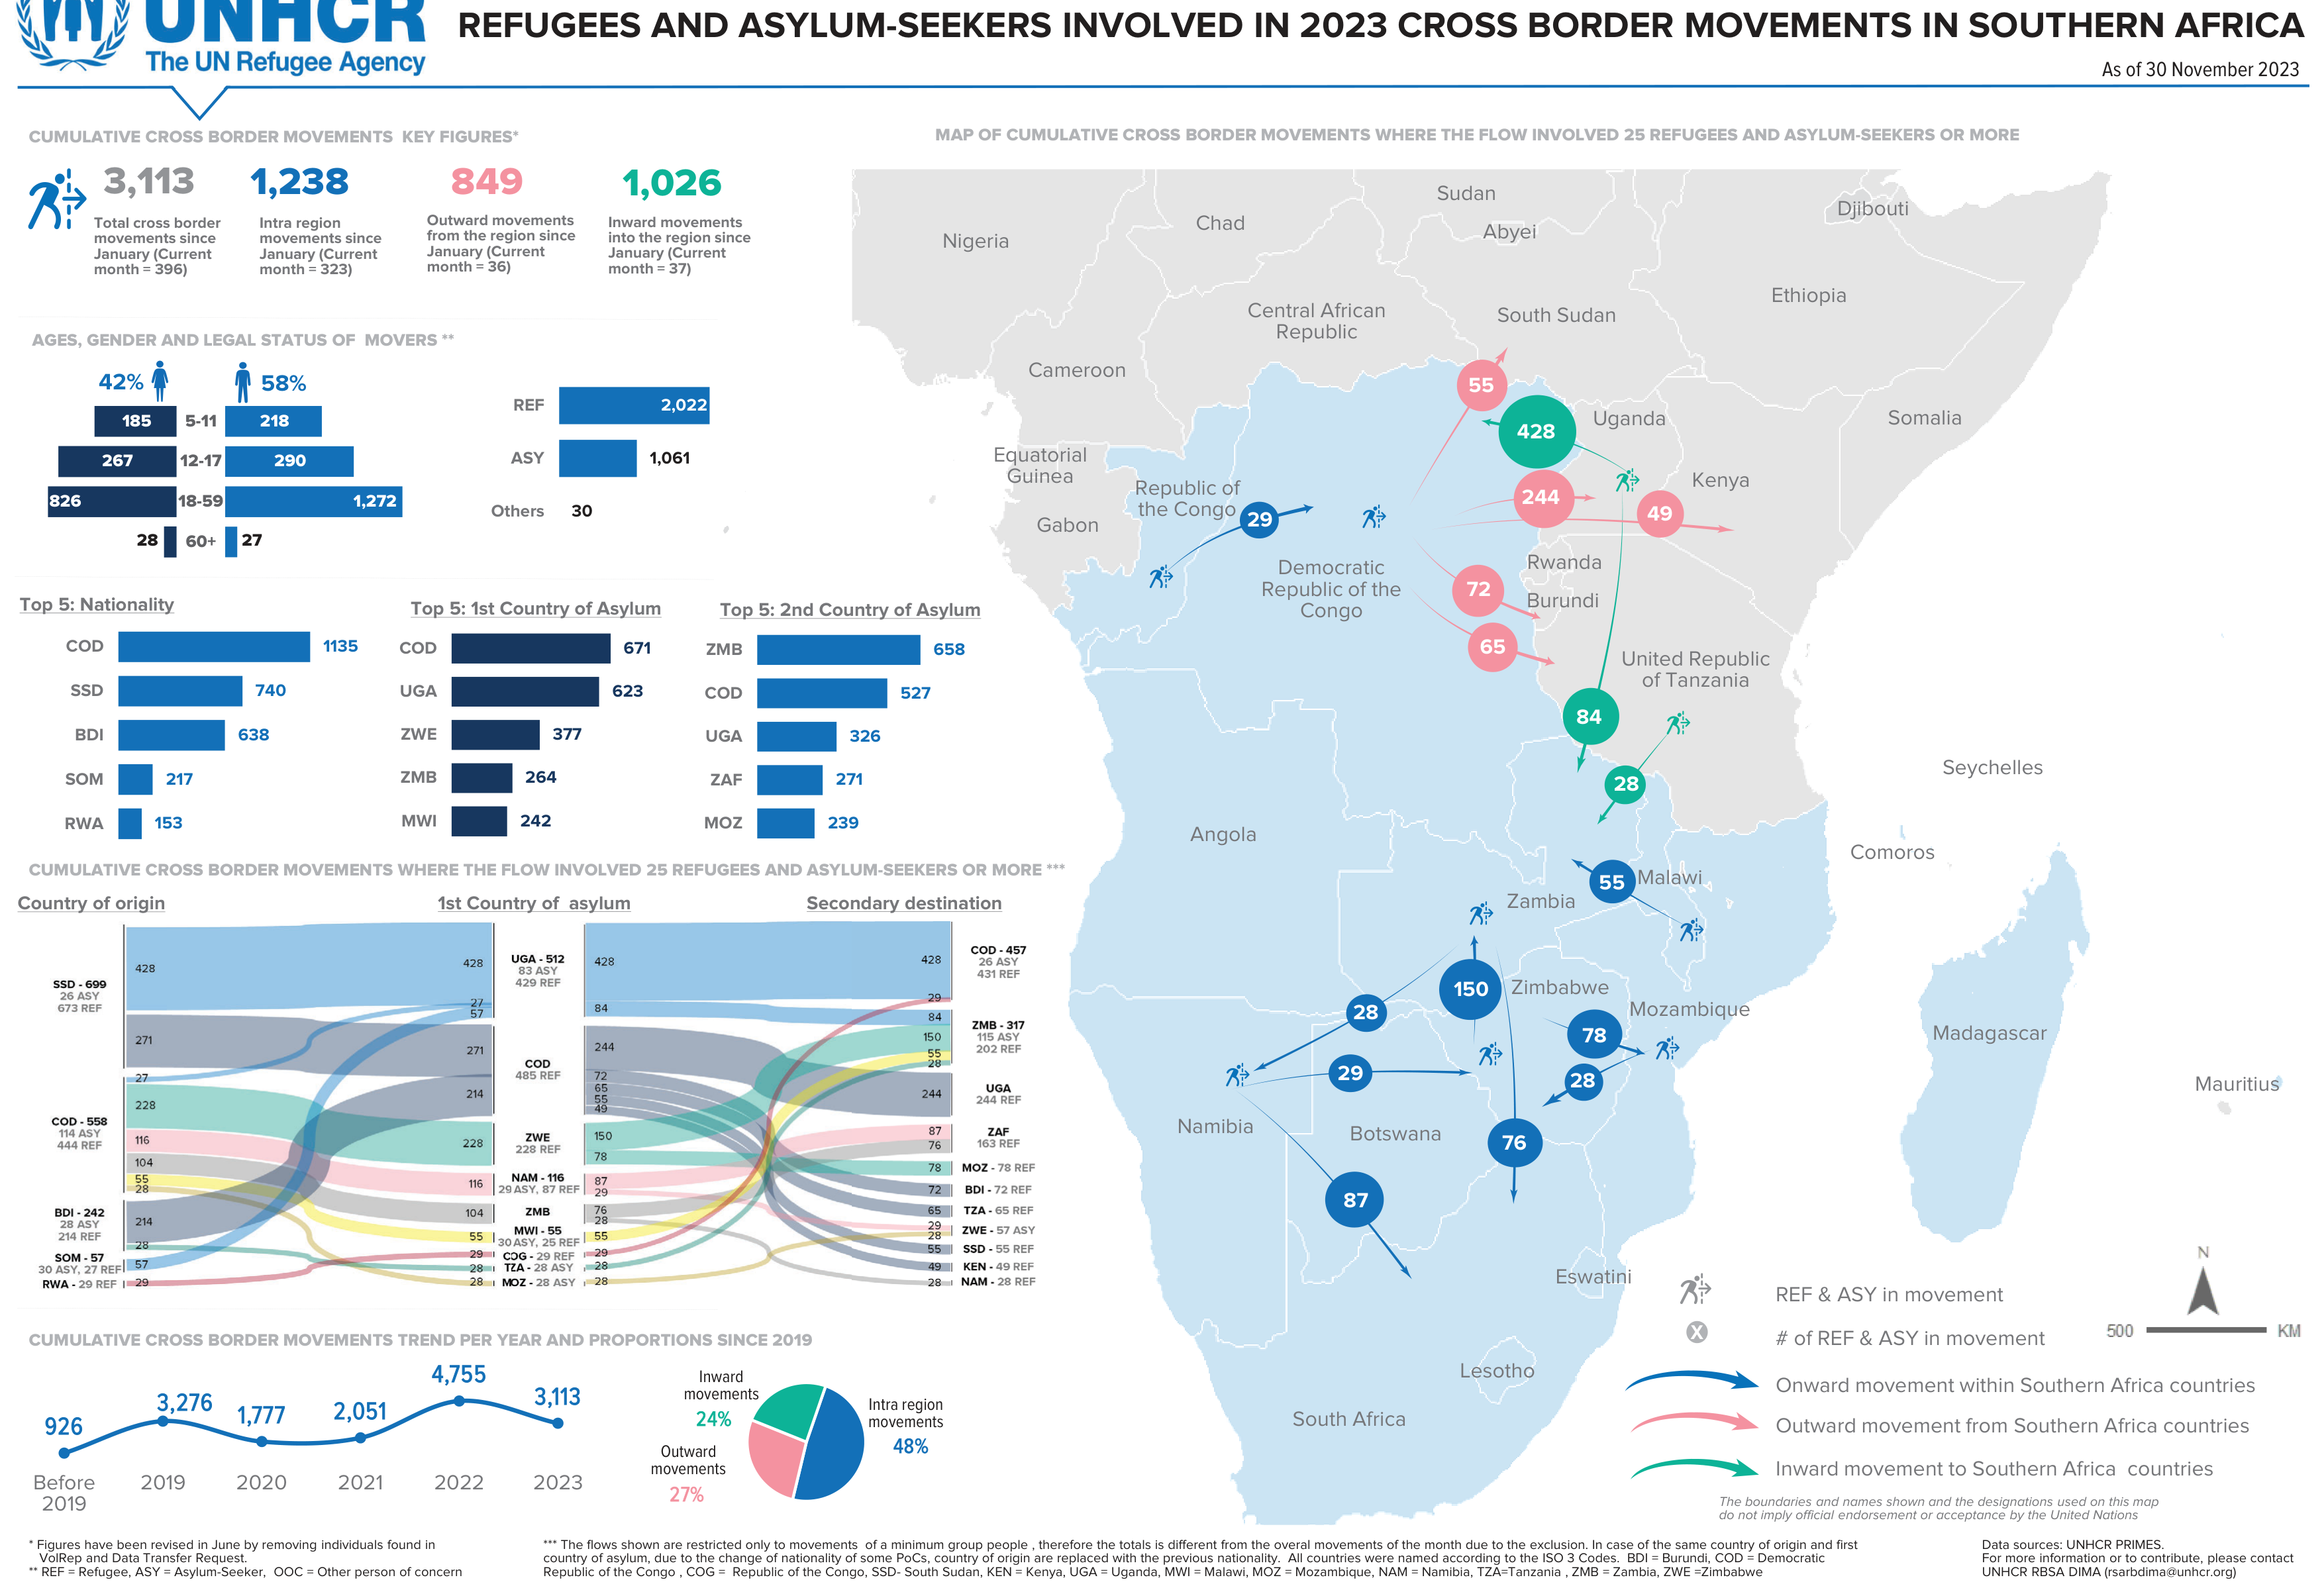
\includegraphics[width=\textwidth]{data/snapshots/nov_2023_rbsa_population_data_analysis_figure_002.png}
    \caption{Representative composite analytical dashboard from the UNHCR / ReliefWeb corpus. The snapshot combines multiple visualization types and analytical components within a single data snapshot.}
    \label{fig:appendix_unhcr_dashboard}
\end{figure}

Figure~\ref{fig:appendix_unhcr_table} presents a representative statistical table extracted from the same corpus. Together with the preceding example, it illustrates the diversity of analytical artifact types treated as data snapshots in this work.

\begin{figure}[!ht]
    \centering
    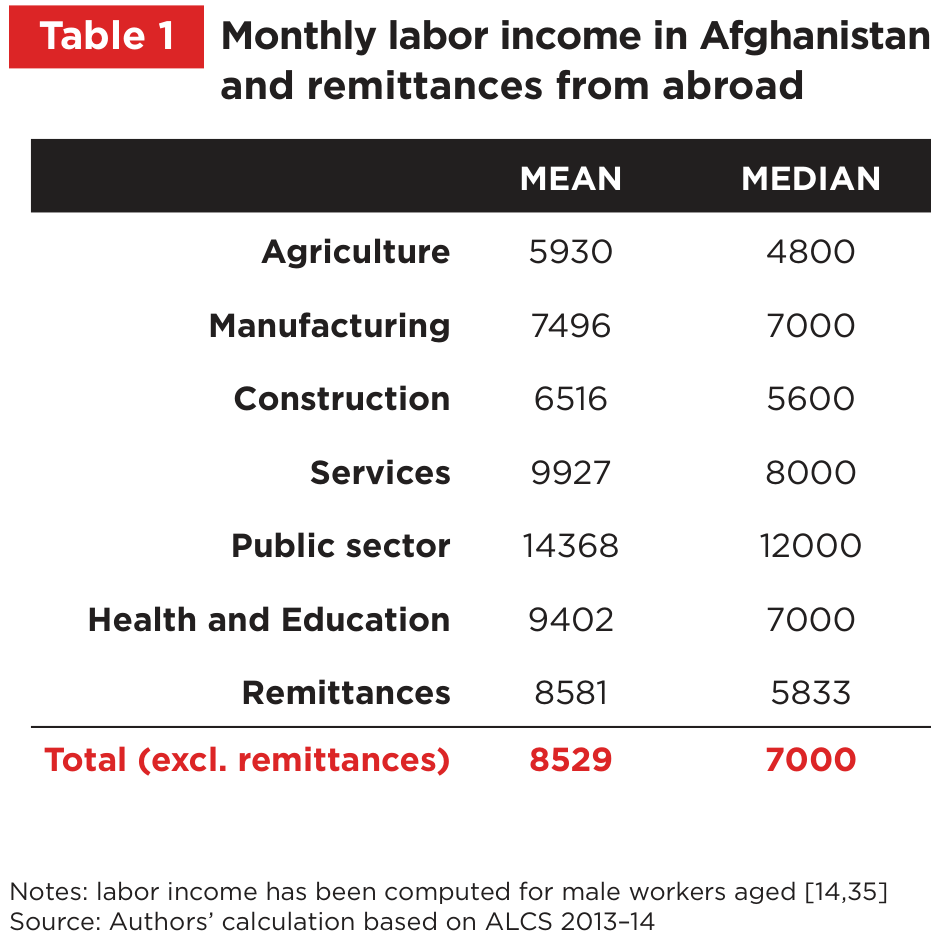
\includegraphics[width=0.5\textwidth]{data/snapshots/108733-revised-public-wb-unhcr-policy-brief-final_table_000.png}
    \caption{Representative statistical table from the UNHCR / ReliefWeb corpus illustrating a structured tabular data snapshot.}
    \label{fig:appendix_unhcr_table}
\end{figure}

\subsection{Policy Research Working Papers}

Figure~\ref{fig:appendix_prwp_map} presents a representative geospatial analytical visualization extracted from the Policy Research Working Papers corpus. The example illustrates that data snapshots include thematic maps alongside charts, tables, and other forms of analytical visualization.

\begin{figure}[!ht]
    \centering
    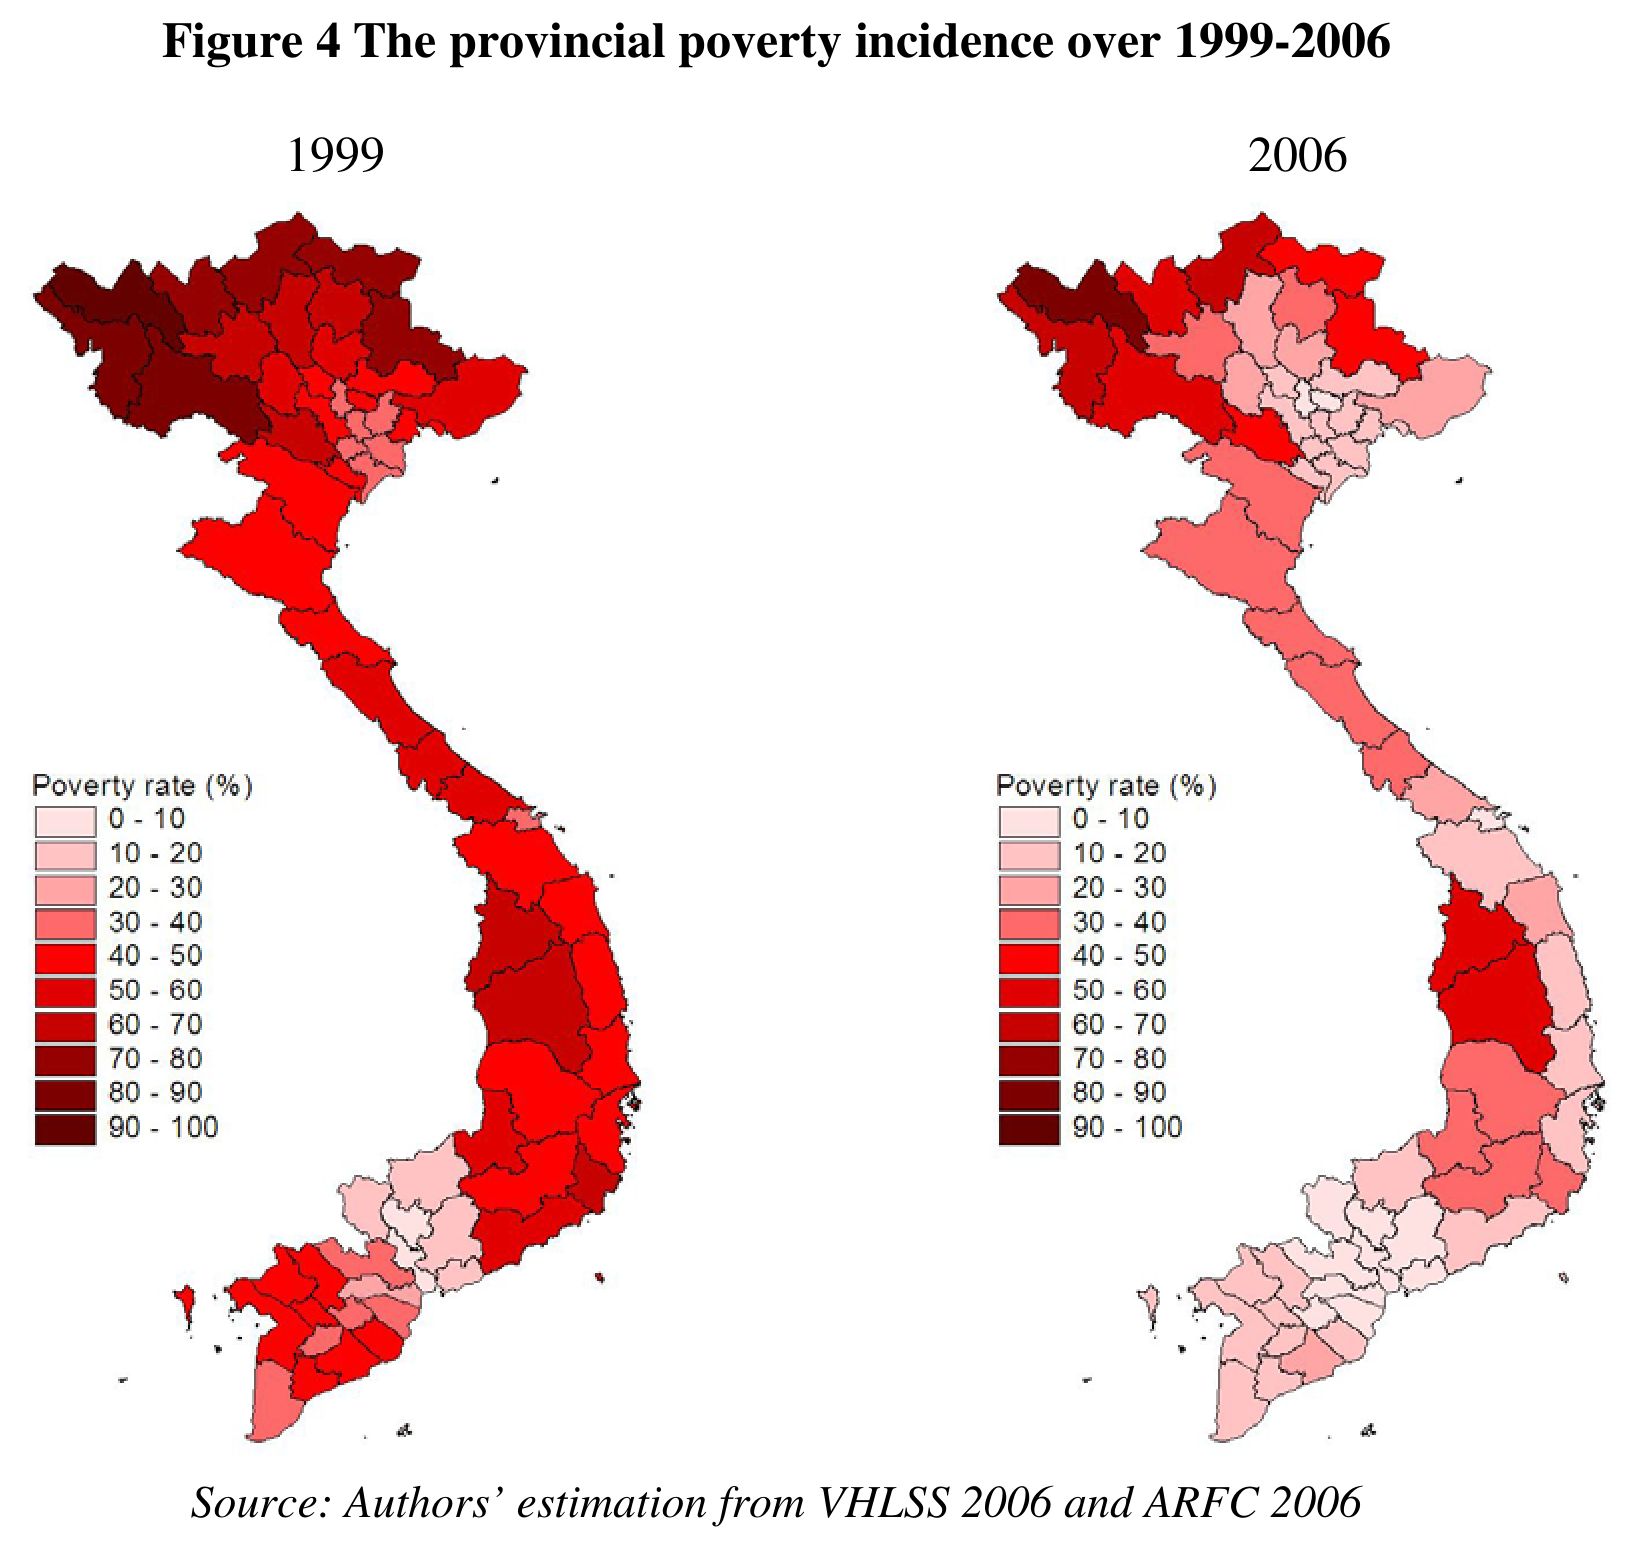
\includegraphics[width=0.5\textwidth]{data/snapshots/document_13148967_figure_003.png}
    \caption{Representative geospatial analytical visualization from the Policy Research Working Papers corpus.}
    \label{fig:appendix_prwp_map}
\end{figure}

Figure~\ref{fig:appendix_prwp_table} presents a representative statistical table extracted from the Policy Research Working Papers corpus. The example illustrates the structured tabular presentation of variables and quantitative information commonly found in academic policy research.

\begin{figure}[!ht]
    \centering
    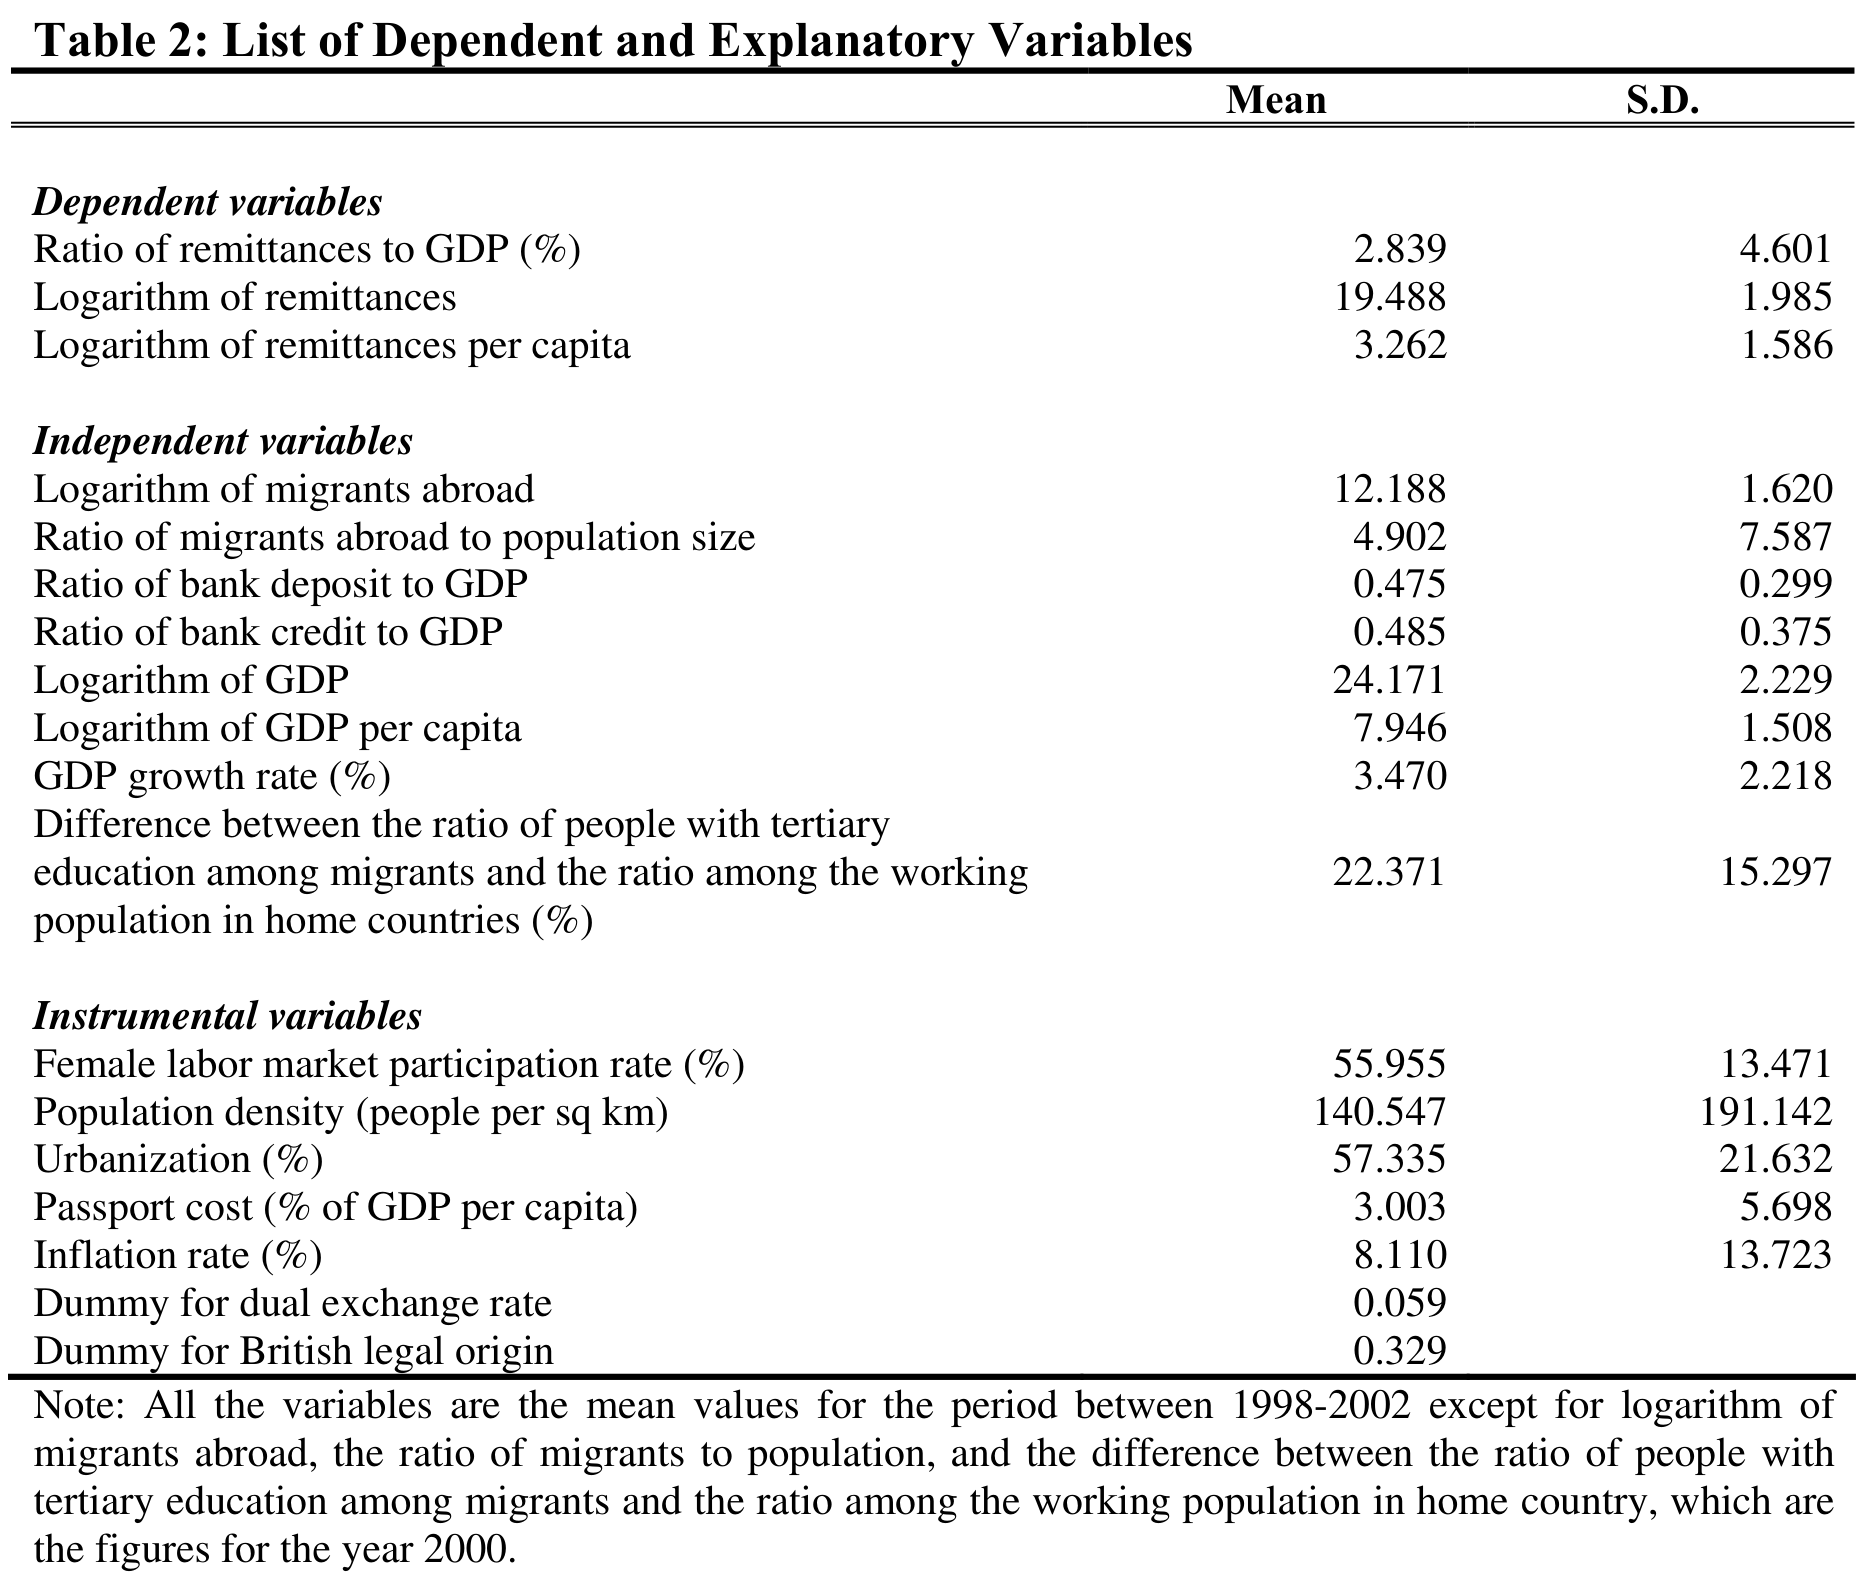
\includegraphics[width=0.5\textwidth]{data/snapshots/document_7255556_table_001.png}
    \caption{Representative statistical table from the Policy Research Working Papers corpus.}
    \label{fig:appendix_prwp_table}
\end{figure}

\subsection{Refugee Project Appraisal Documents}

Figure~\ref{fig:appendix_pad_chart} presents a representative multi-panel statistical visualization extracted from a Refugee Project Appraisal Document. The example illustrates the use of coordinated line charts to compare related indicators across multiple categories within a single analytical figure.

\begin{figure}[!ht]
    \centering
    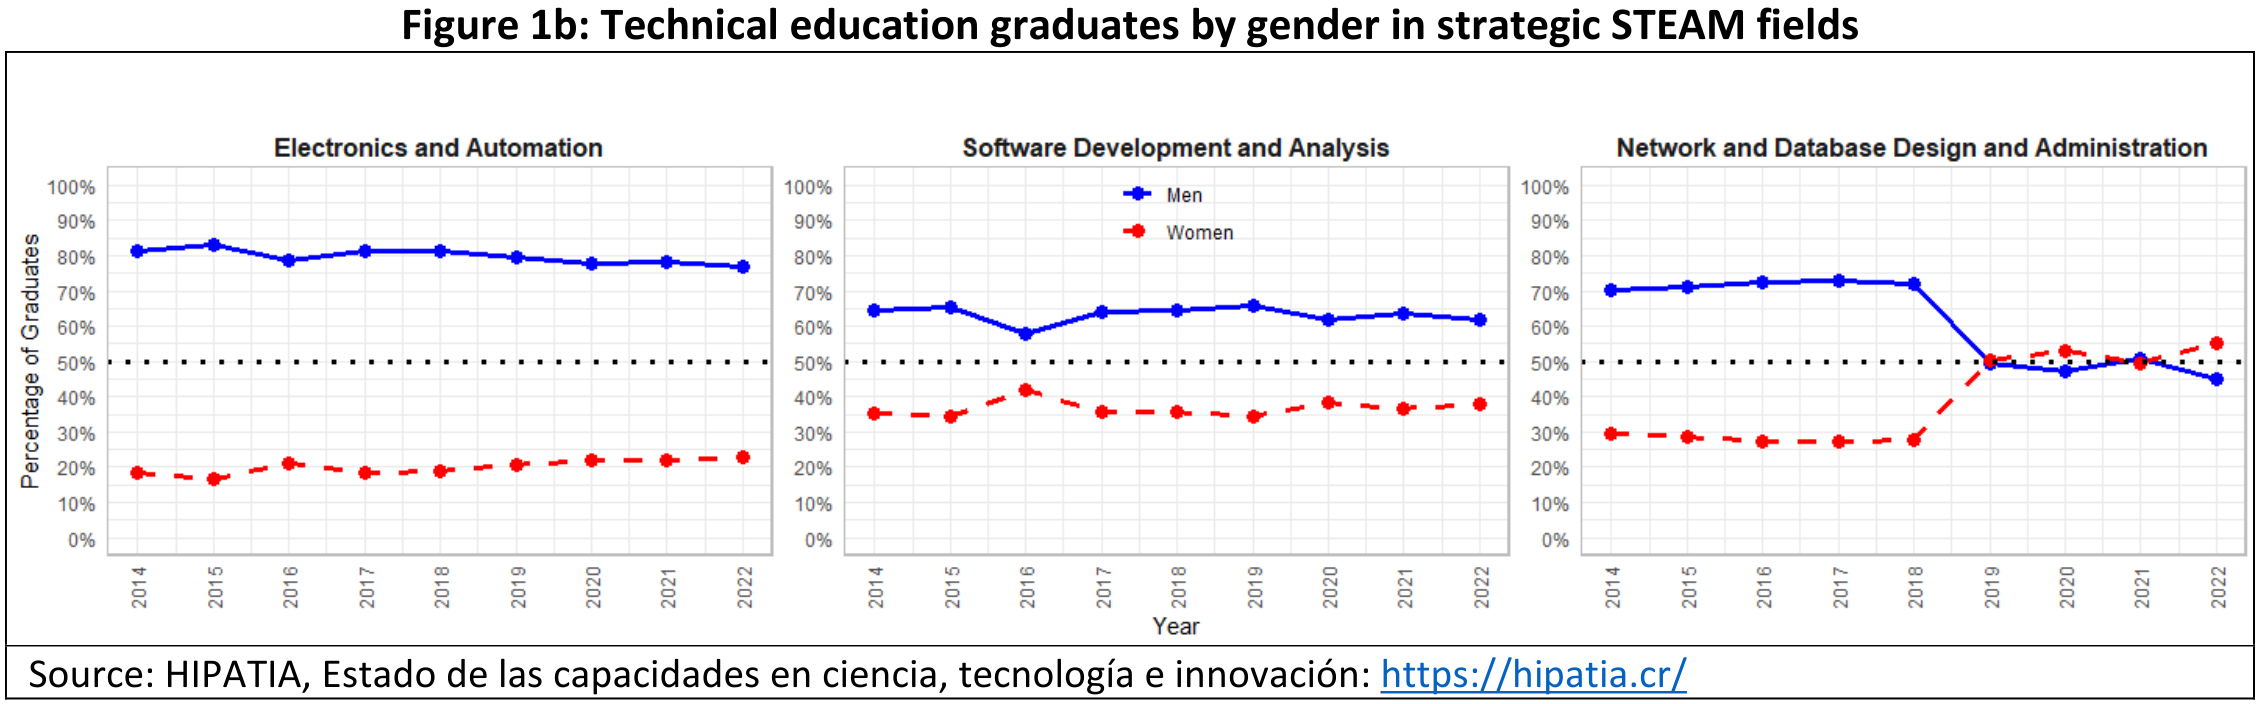
\includegraphics[width=0.75\textwidth]{data/snapshots/005_BOSIB-8191b179-7209-4faa-b5e0-11783bcd492d_figure_001.png}
    \caption{Representative multi-panel statistical visualization from the Refugee Project Appraisal Documents corpus.}
    \label{fig:appendix_pad_chart}
\end{figure}

Figure~\ref{fig:appendix_pad_table} presents a representative project financing table extracted from a Refugee Project Appraisal Document. The example illustrates the structured presentation of financial and operational information commonly found in development project documentation.

\begin{figure}[!ht]
    \centering
    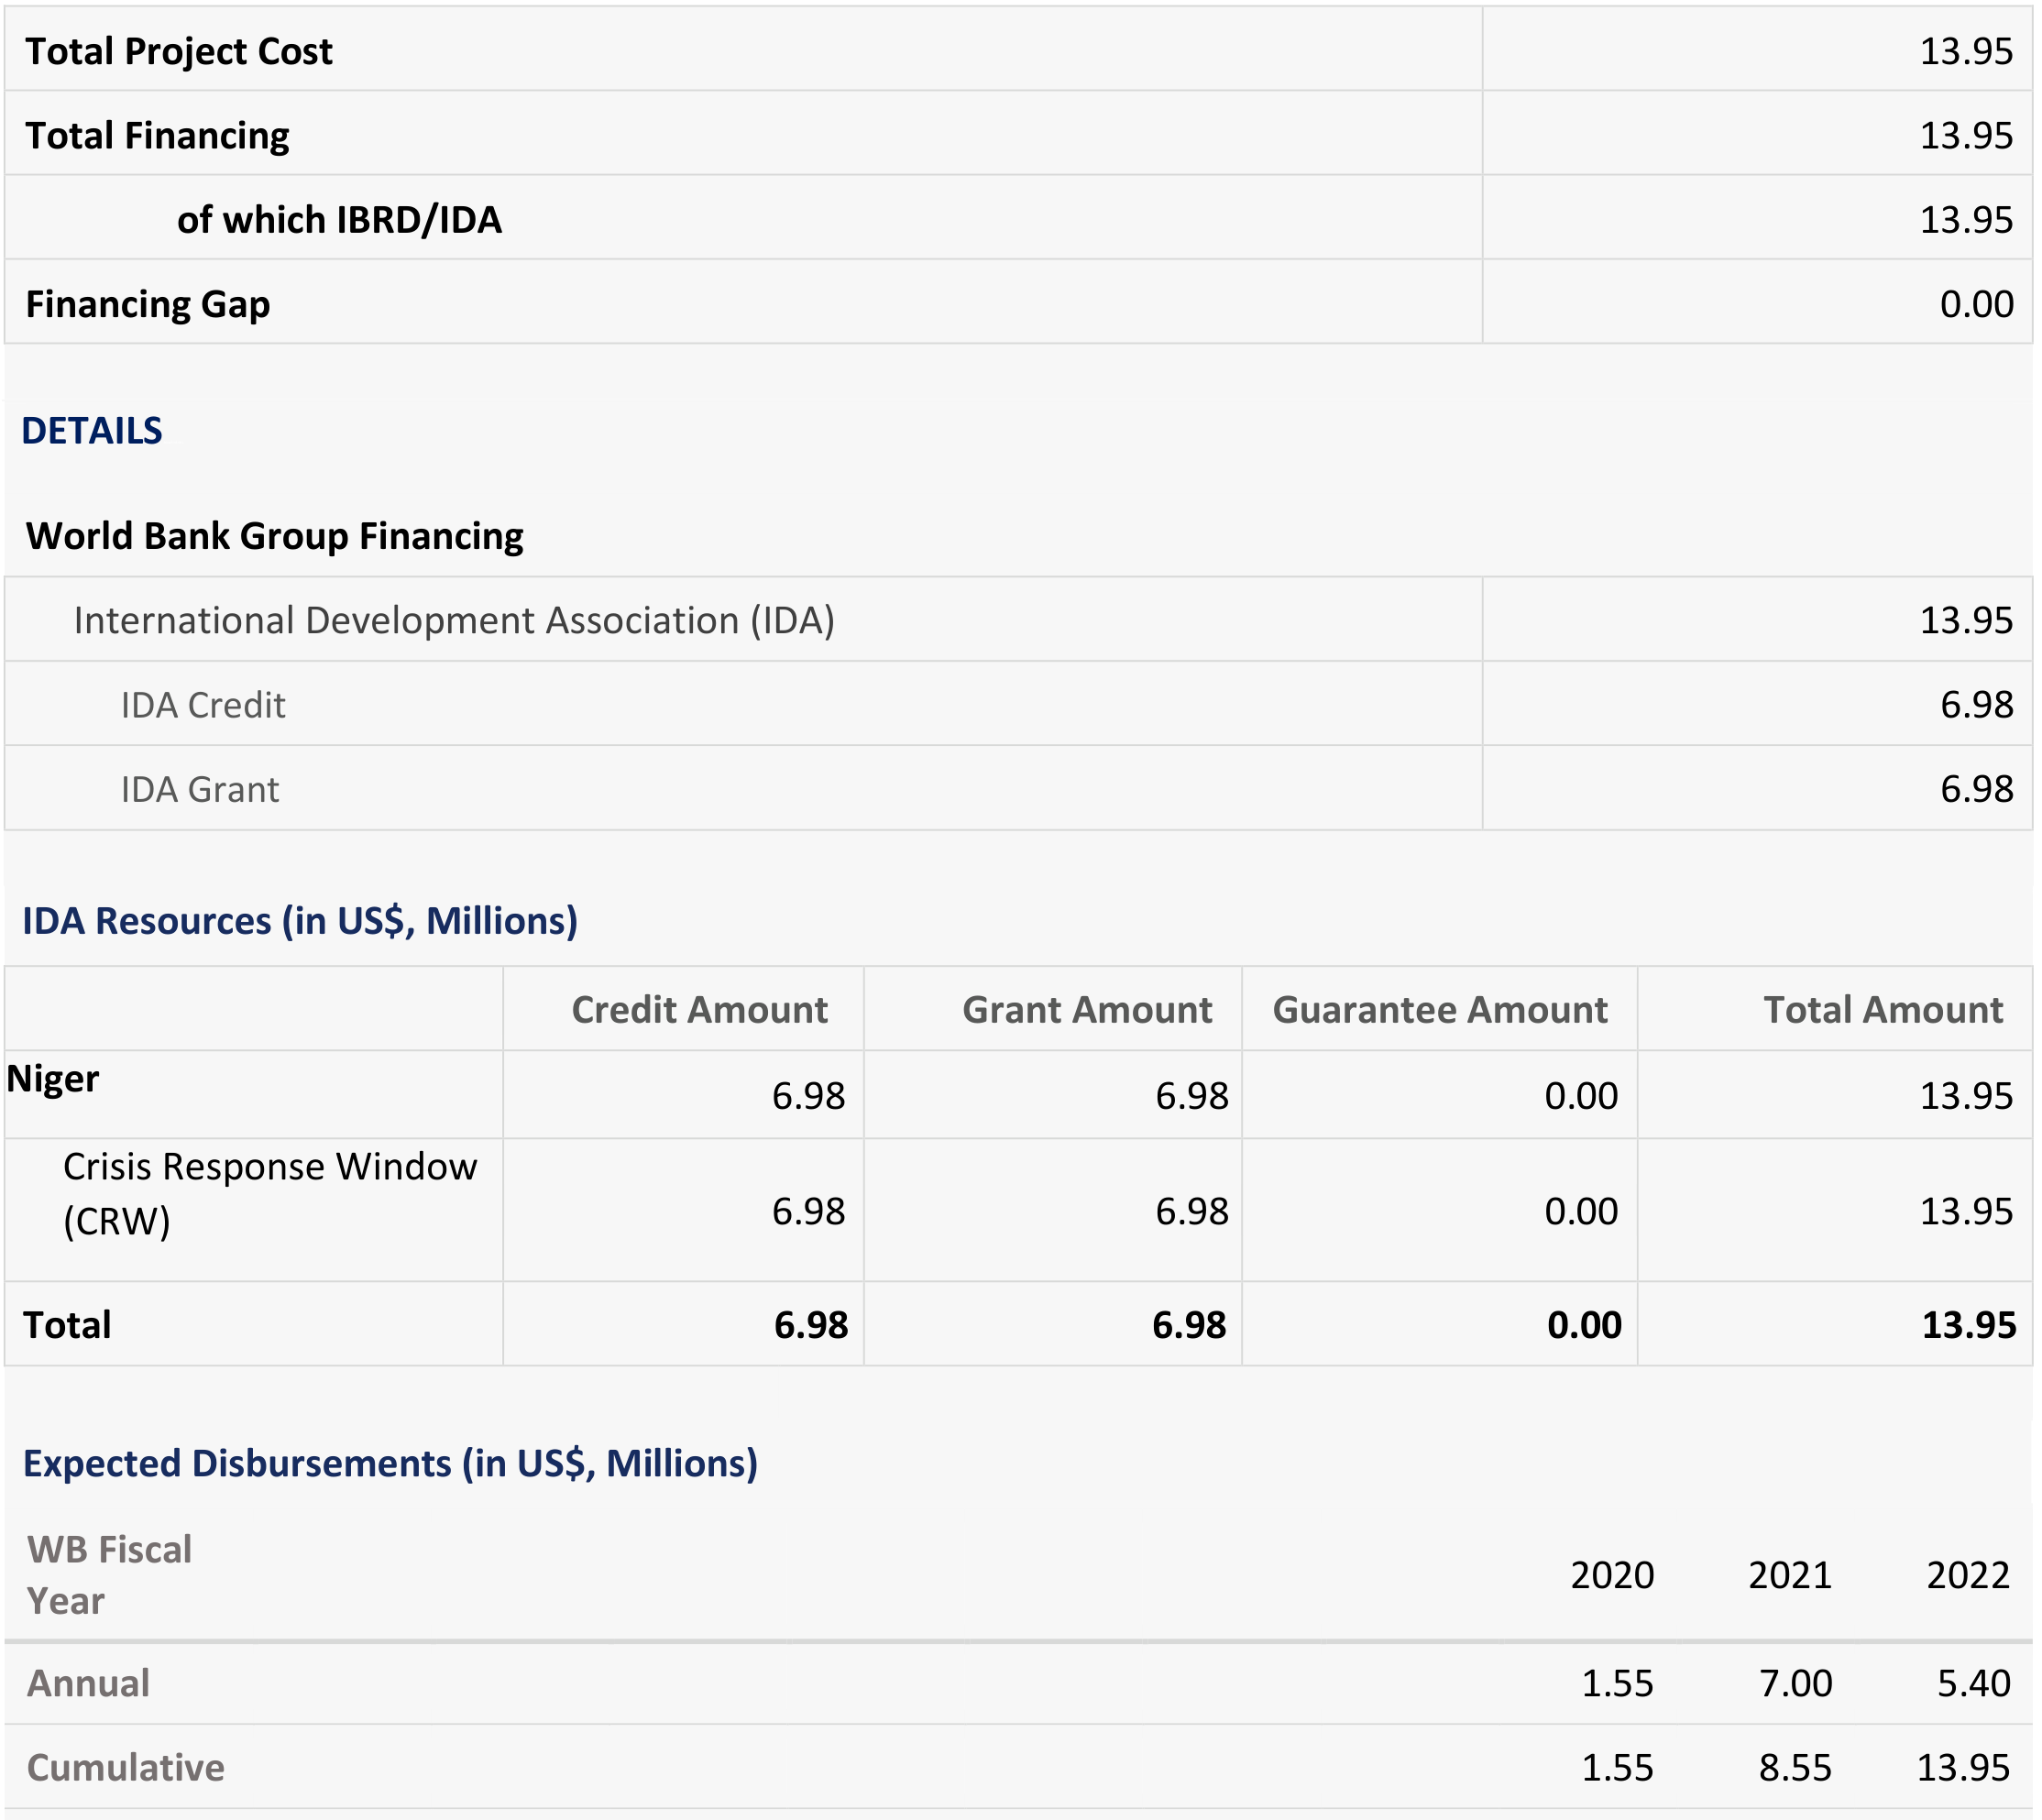
\includegraphics[width=0.6\textwidth]{data/snapshots/056_Niger-COVID-19-Emergency-Response-Project_table_003.png}
    \caption{Representative project financing table from the Refugee Project Appraisal Documents corpus.}
    \label{fig:appendix_pad_table}
\end{figure}

\section{Appendix: Metadata discovery implementation}
\label{appendix:discovery}

This appendix documents the implementation of the metadata discovery stage in the case study. Metadata discovery transforms representative data snapshots into reusable metadata observations that serve as the empirical foundation for field profile aggregation and canonical metadata concept synthesis.

\subsection{Model configuration}

Metadata discovery was performed using GPT-5.5 through the OpenAI Responses API. Table~\ref{tab:metadata_discovery_configuration} summarizes the model configuration used throughout the case study.

\begin{table}[!ht]
    \centering
    \caption{Configuration used for metadata discovery.}
    \label{tab:metadata_discovery_configuration}
    \begin{tabular}{ll}
    \toprule
    \textbf{Setting} & \textbf{Value} \\
    \midrule
    Model & GPT-5.5 \\
    Reasoning effort & Medium \\
    Maximum output tokens & 5000 \\
    Temperature & Default API setting \\
    \bottomrule
    \end{tabular}
\end{table}

\subsection{Implementation}

Representative data snapshots were sampled from the three document corpora described in Section~\ref{sec:case_study}. For each corpus, 35 figures and 35 tables were selected through random sampling, producing a balanced dataset of 210 representative data snapshots.

Each snapshot was processed independently. The snapshot image, together with its associated document-level metadata, was submitted to GPT-5.5 using system and user prompts. Responses were recorded as structured JSON objects and written to disk for subsequent workflow stages.

Processing snapshots independently ensured that metadata discovery for one artifact could not influence the observations produced for any other artifact.

\subsection{Prompt design rationale}

The metadata discovery prompt was designed to elicit reusable metadata concepts rather than perform metadata extraction. Instead of populating a predefined schema, the model was instructed to behave as a metadata architect responsible for proposing candidate metadata fields that could contribute to a future metadata schema.

Several design principles were incorporated into the prompt. First, the model was instructed to distinguish reusable metadata concepts from snapshot-specific values, encouraging abstraction toward canonical metadata fields rather than enumerating observed categories or numerical values. Second, the prompt explicitly distinguished information available from document metadata from information that must be obtained from the snapshot itself, thereby emphasizing metadata that enriches document-level description. Third, the model was instructed to prioritize metadata concepts supporting retrieval, cataloging, provenance, and analytical reuse while de-emphasizing visual formatting and implementation-specific metadata. Finally, hallucination prevention guidelines required observed values to remain grounded in either the snapshot image or the accompanying document metadata, with uncertain values explicitly marked as not identifiable rather than inferred without evidence.

The resulting metadata observations therefore constitute reusable semantic hypotheses about candidate metadata fields rather than extracted metadata records.

\subsection{Reproducibility materials}

The complete system and user prompts, structured-output definitions, and executable implementation for this stage are provided in the accompanying repository.

\section{Appendix: Canonical metadata concept synthesis implementation}
\label{appendix:ontology_induction}

This appendix documents the implementation of canonical metadata concept synthesis in the case study. The original implementation called this stage \emph{ontology induction}; that historical terminology is retained in the implementation artifacts provided in the accompanying repository. As characterized in this paper, the stage transforms aggregated metadata field profiles into a candidate metadata concept inventory for subsequent expert refinement.

\subsection{Model configuration}

Canonical metadata concept synthesis was performed using GPT-5.5 through the OpenAI Responses API. Table~\ref{tab:ontology_induction_configuration} summarizes the model configuration used in the case study.

\begin{table}[!ht]
    \centering
    \caption{Configuration used for canonical metadata concept synthesis.}
    \label{tab:ontology_induction_configuration}
    \begin{tabular}{ll}
    \toprule
    \textbf{Setting} & \textbf{Value} \\
    \midrule
    Model & GPT-5.5 \\
    Reasoning effort & High \\
    Maximum output tokens & 12000 \\
    Temperature & Default API setting \\
    \bottomrule
    \end{tabular}
\end{table}

\subsection{Implementation}

The metadata field profiles produced during field profile aggregation were exported as a CSV file and provided to GPT-5.5 together with system and user prompts. Concept synthesis was performed in a single inference using the \texttt{client.responses.create} interface.

The response consisted of a Markdown table containing canonical metadata concepts, definitions, rationales, and representative discovered metadata fields. This candidate metadata concept inventory subsequently underwent iterative expert refinement.

\subsection{Prompt design rationale}

The prompt was designed to perform semantic consolidation rather than construct a formal ontology. Instead of preserving every discovered metadata field, the model was instructed to synthesize a concise set of reusable metadata concepts that could describe data snapshots across multiple application domains.

Several design principles were incorporated into the prompt. First, the model was instructed to synthesize concepts applicable across multiple reporting domains rather than optimize for a single corpus. Second, it distinguished reusable metadata concepts from observed values and extraction artifacts. Third, the prompt emphasized concepts that support discovery, retrieval, provenance, and analytical reuse while discouraging visual-formatting concepts and duplication of document-level metadata. Finally, it favored under-consolidation over aggressive merging. This preserved plausible distinctions for expert review.

The resulting candidate metadata concept inventory is an intermediate knowledge artifact representing the discovered metadata space rather than a formal ontology or operational metadata schema.

\subsection{Reproducibility materials}

The complete system and user prompts, structured-output definitions, and executable implementation for this stage are provided in the accompanying repository.

\section{Appendix: Concept coverage assessment implementation}
\label{appendix:validation}

This appendix documents the implementation of concept coverage assessment in the case study. The original implementation called this stage \emph{ontology validation}; that historical terminology is retained in the implementation artifacts provided in the accompanying repository. The historical output label \texttt{not\_in\_ontology} corresponds to the residual assignments described in Section~\ref{sec:validation}. As characterized in this paper, the stage assigns each metadata field profile to one concept in the refined metadata concept inventory, producing the assignments analyzed in that section.

\subsection{Model configuration}

Concept coverage assessment was performed using GPT-5.4 mini through the OpenAI Responses API. Table~\ref{tab:ontology_validation_configuration} summarizes the model configuration used in the case study.

\begin{table}[!ht]
    \centering
    \caption{Configuration used for concept coverage assessment.}
    \label{tab:ontology_validation_configuration}
    \begin{tabular}{ll}
    \toprule
    \textbf{Setting} & \textbf{Value} \\
    \midrule
    Model & GPT-5.4 mini \\
    Reasoning effort & Medium \\
    Maximum output tokens & Default API setting \\
    Temperature & Default API setting \\
    Classification output & Concept-inventory-constrained using a Pydantic enumeration \\
    \bottomrule
    \end{tabular}
\end{table}

\subsection{Implementation}

Concept coverage assessment iterated over each metadata field profile produced during field profile aggregation. For each profile, GPT-5.4 mini received system and user prompts together with: (1) the refined metadata concept inventory represented in Markdown, (2) the metadata field name, and (3) representative descriptions and observed values associated with the field profile.

Classification outputs were constrained using a Pydantic enumeration containing every canonical concept together with the historical \texttt{not\_in\_ontology} category. Consequently, every metadata field profile was assigned to exactly one concept or to \texttt{not\_in\_ontology} when no concept adequately described the field.

The resulting concept assignments formed the concept coverage evidence used in the empirical analyses presented in Section~\ref{sec:validation}.

\subsection{Prompt design rationale}

Unlike the previous workflow stages, concept coverage assessment was designed as a constrained classification task rather than an open-ended reasoning task. The prompt instructed the model to treat the refined concept inventory as authoritative and assign each metadata field profile to exactly one existing concept.

Several design principles were incorporated into the prompt. First, the model prioritized semantic meaning over lexical similarity by considering the field name together with representative descriptions and observed values. Second, concept definitions and examples provided contextual guidance but were treated as illustrative rather than exhaustive. Third, the prompt prohibited proposing or modifying concepts so that the assessment characterized the refined inventory rather than extending it. Finally, \texttt{not\_in\_ontology} allowed intentionally excluded fields to be classified without forcing inappropriate assignments.

The resulting classifications constitute concept coverage evidence describing how well the refined inventory accounts for the metadata field profiles produced during field profile aggregation.

\subsection{Reproducibility materials}

The complete system and user prompts, structured-output definitions, and executable implementation for this stage are provided in the accompanying repository.

\section{Appendix: Held-out schema validation implementation}
\label{appendix:schema_validation}

This appendix documents the two schema-validation exercises applied to the same 202 snapshots held out from metadata discovery through initial schema design and then used for held-out schema validation. The version identifiers and field names in this appendix describe the frozen artifacts and structured outputs used during execution and are therefore retained for reproducibility. Both exercises evaluated one snapshot per request using the snapshot image, the complete frozen schema, and available source-document metadata. Neither exercise permitted the model to revise the schema or accept a proposed field.

\subsection{Validation 1: Open residual discovery}

\subsubsection{Model configuration}

Validation 1 used GPT-5.5 through the OpenAI Responses API. Table~\ref{tab:schema_validation1_configuration} summarizes the final configuration used for the full held-out run.

\begin{table}[!ht]
    \centering
    \caption{Configuration used for Schema Validation 1.}
    \label{tab:schema_validation1_configuration}
    \begin{tabular}{ll}
    \toprule
    \textbf{Setting} & \textbf{Value} \\
    \midrule
    Frozen schema & Data Snapshot Metadata Schema v1.1 \\
    Model & GPT-5.5 \\
    Reasoning effort & Medium \\
    Service tier & Flex \\
    Maximum output tokens & 8,000 \\
    Prompt caching & Enabled \\
    Assessment unit & One held-out snapshot per request \\
    Output & Pydantic Structured Output \\
    \bottomrule
    \end{tabular}
\end{table}

\subsubsection{Assessment and output structure}

The exercise used open residual discovery. For each snapshot, the model independently identified reusable metadata concepts, compared them with the frozen schema, and returned one evidence-bearing observation for each concept substantively relevant to coverage. Each observation contained an identifier, the metadata concept, explicit evidence and its source, the closest schema fields, a fit status, and a concise rationale.

The fit statuses were defined as follows:

\begin{itemize}
    \item \texttt{covered}: one or more existing fields represented the concept without material loss;
    \item \texttt{weak\_fit}: an existing field was related, but using it would distort, omit, or conflate important semantics;
    \item \texttt{no\_fit}: the concept was within scope and no existing field adequately represented it;
    \item \texttt{out\_of\_scope}: the observation was extraction output or otherwise outside snapshot metadata; and
    \item \texttt{uncertain}: the evidence or semantic interpretation was insufficient for a reliable decision.
\end{itemize}

The structured output contained two arrays: \texttt{observations} and \texttt{candidate\_new\_fields}. A candidate contained a proposed name, definition, supporting observation identifiers, an explanation of why existing fields were insufficient, its operational value, and its source level. The output contract required every candidate to be supported by at least one \texttt{weak\_fit} or \texttt{no\_fit} observation. Across the 202 requests, the model returned 2,876 observations and 578 candidate objects using 101 exact proposed names. Because snapshots were assessed independently, semantically related candidates could recur within or across exact names. The 578 figure is therefore the number of candidate objects returned across snapshots, not the number of accepted fields or unique names.

\subsubsection{Human adjudication}

Candidate names were not normalized by the model. Human review manually grouped obvious semantic aliases into 14 provisional review families. These families covered 518 of the 578 candidate rows and served only as an analysis aid; they were not treated as model output or as a new schema layer. The reviewer examined all 14 families, the remaining 60 ungrouped candidate rows, and all 23 boundary-quality observations classified as \texttt{uncertain} or \texttt{out\_of\_scope}.

Acceptance was not determined by candidate frequency. For each candidate area, the reviewer considered whether the evidence described the snapshot rather than only its source document, whether the concept was reusable and within scope, whether existing fields already represented it adequately, whether it was metadata rather than extracted analytical content, whether an independent field had operational value, and whether the issue concerned missing vocabulary or the representation of an existing concept. Application architecture, expected retrieval behavior, generalizability, and maintenance cost informed the operational decision. Decisions and rationales were recorded by candidate area in the final adjudication report. No candidate was accepted as a new field.

\subsubsection{Reproducibility materials}

The complete system and user prompts, structured-output definitions, and executable implementation for this stage are provided in the accompanying repository.

\subsection{Validation 2: Confirmatory critical-gap assessment}

\subsubsection{Model configuration}

Validation 2 also used GPT-5.5 through the OpenAI Responses API, but applied a narrower assessment to the documentation-revised schema. Table~\ref{tab:schema_validation2_configuration} summarizes the final configuration. The model-facing schema retained the complete field specification but omitted validation-history language to reduce anchoring on the earlier result.

\begin{table}[!ht]
    \centering
    \caption{Configuration used for Schema Validation 2.}
    \label{tab:schema_validation2_configuration}
    \begin{tabular}{ll}
    \toprule
    \textbf{Setting} & \textbf{Value} \\
    \midrule
    Frozen schema & Data Snapshot Metadata Schema v1.1.1 \\
    Model & GPT-5.5 \\
    Reasoning effort & Medium \\
    Service tier & Flex \\
    Maximum output tokens & 8,000 \\
    Prompt caching & Enabled \\
    Assessment unit & One held-out snapshot per request \\
    Output & Pydantic Structured Output \\
    \bottomrule
    \end{tabular}
\end{table}

\subsubsection{Assessment and output structure}

Validation 2 asked whether a snapshot contained any critical or possibly critical reusable metadata that the schema could not represent adequately and whose absence would materially impair interpretation, discovery, or both. A \texttt{critical} gap required explicit evidence, reusable snapshot metadata, no adequate existing field, and a concrete material impact. A \texttt{possible} gap required plausible reusable metadata and plausible material impact, but retained uncertainty about the evidence, existing-field coverage, or materiality. Information that was merely useful, convenient, specialized, or an additional search facet did not meet either threshold.

The structured output contained a snapshot-level \texttt{coverage\_assessment} and a \texttt{critical\_or\_possible\_gaps} array. The assessment was \texttt{no\_critical\_gap\_found}, \texttt{critical\_gap\_found}, or \texttt{possible\_gap}. Each candidate gap recorded its status, missing concept, proposed field name, evidence, justification as snapshot metadata, closest schema fields, possible semantic loss, material-impact category, concrete consequence, and any remaining uncertainty. Consistency rules required an empty array for \texttt{no\_critical\_gap\_found}, at least one critical gap for \texttt{critical\_gap\_found}, and one or more possible but no critical gaps for \texttt{possible\_gap}.

\subsubsection{Human adjudication}

Human review examined all six possible-gap records returned across five snapshots. The reviewer assessed whether the information was evidenced, reusable snapshot metadata, adequately represented by existing fields, materially important to interpretation or discovery, and generalizable beyond a specialized artifact. The reviewer also determined whether each candidate represented a missing concept, a documentation concern, or a structural representation limitation. Candidate frequency was supporting evidence rather than an acceptance rule.

Adjudication was recorded by snapshot filename and gap identifier using the fields \texttt{human\_decision}, \texttt{critical\_to\_interpretability}, \texttt{critical\_to\_discoverability}, and \texttt{human\_rationale}. The final report recorded the decision and rationale for each of the six candidates. None was accepted as a new field; four were rejected or excluded, and two were classified as representation limitations. The 197 \texttt{no\_critical\_gap\_found} assessments did not receive an independent human false-negative audit.

\subsubsection{Reproducibility materials}

The complete system and user prompts, structured-output definitions, and executable implementation for this stage are provided in the accompanying repository.

\section{Appendix: Standards-informed schema refinement}
\label{appendix:standards_refinement}

The standards review was conducted as an interactive, multi-turn Codex task rather than as a single fixed-prompt inference call. The validated flat schema, schema-validation findings, and relevant repository documentation provided the local context. Standards claims and candidate mappings were grounded in authoritative documentation for the reviewed standards.

\begin{table}[!ht]
    \centering
    \caption{Configuration used for standards-informed schema refinement.}
    \label{tab:standards_refinement_configuration}
    \begin{tabular}{ll}
        \toprule
        \textbf{Setting} & \textbf{Value} \\
        \midrule
        Interface & Codex Desktop \\
        Model & GPT 5.6 Sol \\
        Reasoning effort & High \\
        Interaction mode & Interactive, multi-turn review \\
        Input schema & Validated 36-field flat specification \\
        Supporting evidence & Schema-validation findings and adjudication \\
        External evidence & Authoritative standards documentation \\
        Outputs & Field crosswalk, candidate refinements, and decision record \\
        \bottomrule
    \end{tabular}
\end{table}

Table~\ref{tab:standards_sources} records the authoritative sources used in the crosswalk. Fixed versions or publication dates are reported only where the source establishes them; mutable sources are identified by the date on which they were verified or accessed.

\begin{table}[!ht]
    \centering
    \caption{Authoritative sources used for standards-informed schema refinement.}
    \label{tab:standards_sources}
    \renewcommand{\arraystretch}{1.15}
    \scriptsize
    \begin{tabularx}{\textwidth}{>{\RaggedRight\arraybackslash}p{0.14\textwidth} >{\RaggedRight\arraybackslash}p{0.26\textwidth} >{\RaggedRight\arraybackslash}p{0.23\textwidth} >{\RaggedRight\arraybackslash}X}
        \toprule
        \textbf{Standard or vocabulary} & \textbf{Authoritative source} & \textbf{Version or source date} & \textbf{Crosswalk role} \\
        \midrule
        DCMI & DCMI Metadata Terms~\citep{dcmi2020terms} & Recommendation dated 2020-01-20 & General resource description \\
        Schema.org & Schema.org vocabulary and term pages~\citep{schemaorg2026} & Version not recorded; verified/accessed 2026-09-23 & Cross-domain resource, dataset, and measurement properties \\
        DCAT & Data Catalog Vocabulary (DCAT) 3~\citep{albertoni2024dcat3} & W3C Recommendation dated 2024-08-22 & Catalog, spatial, and temporal description \\
        SDMX & SDMX technical standards and cross-domain concepts~\citep{sdmx2025standards} & Version 3.1, released May 2025 & Statistical dimensions, frequency, time, and units \\
        DDI & DDI Lifecycle and controlled vocabularies~\citep{ddi2020lifecycle33} & Lifecycle 3.3; documentation dated 2020-01-15 & Variables, universe, categories, geography, collection, and summary statistics \\
        PROV-O & PROV-O: The PROV Ontology~\citep{lebo2013provo} & W3C Recommendation dated 2013-04-30 & Derivation and attribution provenance \\
        JATS & Journal Publishing Tag Set 1.3~\citep{niso2021jats13} & Approved 2021-06-10 & Figure labels, captions, and groups \\
        SKOS & SKOS Simple Knowledge Organization System Reference~\citep{miles2009skos} & W3C Recommendation dated 2009-08-18 & Concepts, labels, schemes, and mappings \\
        IATI & IATI Standard documentation~\citep{iati203} & Version 2.03 & Project, finance, organization, and location terms \\
        RDF Data Cube and OWL-Time & W3C Data Cube vocabulary and Time Ontology~\citep{cyganiak2014datacube,cox2017owltime} & Recommendations dated 2014-01-16 and 2017-10-19 & Statistical dimensions and temporal representation \\
        ISO and UN value standards & ISO 8601, ISO 3166, ISO 4217, and UN M49~\citep{iso8601,iso3166,iso4217,unm49} & 8601-1:2019; 3166 version not recorded; 4217:2015; M49 version not recorded; accessed 2026-09-23 & Dates, country and area identifiers, and currencies \\
        Other value and visualization references & BCP 47, UN/CEFACT Recommendation 20, and Vega-Lite~\citep{ietf2009bcp47,uncefactrec20,vegalite2026} & BCP 47 current subseries; other versions not recorded; accessed 2026-09-23 & Languages, units of measure, and visualization terminology \\
        \bottomrule
    \end{tabularx}
\end{table}

The review first identified standards applicable to general resource description, statistical and research-data concepts, provenance, document publishing, development-project information, and value normalization. Each schema field was compared with candidate external terms and classified as exact, close, broader, narrower, related or structural, or having no direct match. Candidate refinements could concern field terminology, definitions, semantic boundaries, value guidance, or representation structure.

The proposed mappings and refinements were then reviewed against the artifact evidence, validation findings, intended application, and requirement that the paper specification remain directly inspectable. Accepted changes were incorporated into the final specification. Proposals that narrowed or distorted observed concepts were rejected, and richer relational or machine-enforceable structures were deferred. The accompanying repository provides the complete field-level crosswalk, decision matrix, and resulting standards-informed specification.

\section{Appendix: Data Snapshot Metadata Schema}
\label{appendix:schema}

This appendix reproduces the complete standards-informed Data Snapshot Metadata Schema produced by the methodology. Version identifiers are retained within the reproduced artifact.

\begin{lstlisting}
# Data Snapshot Metadata Schema v1.1.2

Status: Standards-informed flat specification

## Overview

The Data Snapshot Metadata Schema v1.1.2 defines 37 metadata fields for
describing a data snapshot: a self-contained table, chart, map, dashboard, or
composite figure extracted from an institutional document.

The schema remains flat so that its fields, definitions, and populated records
can be inspected directly. Standards alignment refines its terminology,
semantic boundaries, and usage guidance without requiring one external
vocabulary to cover every field.

## Revision notes

Version 1.1.2 is a standards-informed revision of the validated v1.1.1 schema.
It:

- preserves the accepted information coverage;
- adopts clearer application-facing field names where the standards review
  identified ambiguity or multiplicity;
- splits the overloaded `data_source` field into `data_sources` and
  `attributions`;
- clarifies the resource, context, and evidence described by each field;
- records relevant standards mappings and value guidance; and
- preserves open source-grounded values when no exact external vocabulary is
  appropriate.

## Scope

The schema describes metadata about one data snapshot. It excludes extracted
numerical observations, OCR text, reconstructed chart data, table-cell
contents, and other content-extraction outputs.

Metadata must be supported by the snapshot or, where a field explicitly
permits it, by relevant source-document context. Snapshot evidence remains
primary. Parent-document URLs, identifiers, document types, publication dates,
authors, and publishers are not duplicated in the snapshot record.

## Applicability and cardinality

Every field is optional because different artifact types expose different
metadata. Missing values are represented as null rather than inferred.

The notation `0..1` indicates an optional single text value. The notation
`0..*` indicates an optional ordered list of text values. The schema does not
encode relationships among values stored in different flat fields.

## Standards-informed representation principles

1. Populate metadata only when supported by explicit evidence.
2. Preserve source-visible terminology when normalization would remove or
   distort information.
3. Use an established term, format, or code only when the mapping is exact and
   remains understandable in the flat field.
4. Do not force a value into a controlled vocabulary when the mapping is
   ambiguous or domain-dependent.
5. Do not infer temporal precision, geographic level, analytical role, or
   semantic relationships that the artifact does not establish.
6. Preserve source order for ordered values and remove only exact duplicates
   within the same field.
7. Do not translate source-visible text as part of metadata recording.

# Schema modules

## Identity and discovery

| Field | Cardinality | Definition | Standards alignment and usage guidance |
|---|---:|---|---|
| `title` | 0..1 | The primary title, caption, or heading that identifies the data snapshot. | Aligns with DCMI `title` and Schema.org `name`. Preserve the snapshot title rather than substituting the parent-document title. |
| `document_label` | 0..1 | The label assigned to the snapshot within its source document. | JATS `label` is the closest pattern; general identifier properties are broader. Use for labels such as "Figure 3" or "Table 4.2," not for global identifiers. |
| `subject_domains` | 0..* | The broad thematic, policy, or sectoral domains represented by the snapshot. | Related to DCMI `subject`, Schema.org `about`, DCAT `theme`, and SKOS concepts. Use recognizable domain labels without requiring one universal vocabulary. |
| `subject_summary` | 0..1 | A concise summary of the snapshot's primary analytical subject or purpose. | Schema.org `abstract` is a close match; DCMI `description` is broader. Summarize the snapshot rather than the parent document. |
| `panel_titles` | 0..* | The titles or headings explicitly shown for individual panels in a multi-panel snapshot. | JATS figure-group and caption-title patterns provide the closest structural analogue. Preserve explicit titles in source order and do not infer titles for unlabeled panels. |

## Subject and semantics

| Field | Cardinality | Definition | Standards alignment and usage guidance |
|---|---:|---|---|
| `variable_names` | 0..* | The variables, indicators, metrics, or measured concepts represented by the snapshot. | Closely aligned with Schema.org `variableMeasured`, DDI Variable, and SDMX measure concepts. Record represented concepts, not inferred analytical roles. |
| `category_dimensions` | 0..* | The conceptual variables or dimensions used to organize, group, classify, or compare represented values. | Closely aligned with SDMX Dimension, DDI RepresentedVariable, and the RDF Data Cube dimension pattern. |
| `category_labels` | 0..* | The explicit category names or labels associated with the represented category dimensions. | SDMX Code/Codelist, DDI Category/CodeList, and SKOS labels provide relevant patterns. Preserve displayed labels and source order; do not add a code without a known scheme. |
| `population_group` | 0..1 | The human population, beneficiary group, or demographic group that is the primary subject of the represented data. | Closely aligned with DDI Universe and Schema.org `populationType`. Describe who the data concern rather than a category used only to organize them. |

## Temporal context

| Field | Cardinality | Definition | Standards alignment and usage guidance |
|---|---:|---|---|
| `time_period` | 0..1 | The date, interval, or source expression describing when the represented data apply. | Aligns with Schema.org `temporalCoverage`, DCMI `temporal`, and SDMX `TIME_PERIOD`. Preserve the complete source expression and do not infer unsupported bounds or precision. |
| `temporal_granularity` | 0..1 | The temporal resolution or reporting interval of the represented data. | SDMX frequency, DCAT temporal resolution, and OWL-Time provide related terminology. Use an SDMX frequency only when exact; preserve irregular or event-based descriptions when appropriate. |

## Spatial context

| Field | Cardinality | Definition | Standards alignment and usage guidance |
|---|---:|---|---|
| `geographic_scope` | 0..1 | The overall place or geographic area that the snapshot principally covers or concerns. | Aligns with Schema.org `spatialCoverage`, DCMI `spatial`, and DCAT spatial coverage. The scope may be broader than the named entities shown within it. |
| `geographic_entities` | 0..* | Named geographic entities explicitly represented within the snapshot. | Closely aligned with Schema.org Place and DDI GeographicLocation. Preserve displayed names; use a standardized name or code only when the mapping is unambiguous. |
| `geographic_level` | 0..1 | The administrative, geographic, or reporting level at which the data are represented. | Closely aligned with DDI GeographicLevel and, where applicable, ISO 3166-2. Do not infer an administrative level without sufficient jurisdictional context. |
| `geographic_roles` | 0..* | The explicit semantic roles played by geographic entities, such as country of origin, host country, or destination. | No reviewed vocabulary provides a universal exact match. Preserve source-grounded roles rather than imposing a closed vocabulary. |
| `location_types` | 0..* | The physical, administrative, or operational kinds of locations represented, such as camp, school, settlement, or district. | IATI LocationType and SKOS provide optional patterns. Do not force an approximate external category. |

## Measurement context

| Field | Cardinality | Definition | Standards alignment and usage guidance |
|---|---:|---|---|
| `units_of_measure` | 0..* | The units needed to interpret the reported quantitative values. | Aligns with SDMX `UNIT_MEASURE`, Schema.org `unitCode`, and UN/CEFACT Recommendation 20. Preserve displayed units and apply a code only when exact. |
| `currencies` | 0..* | The currency denominations used for monetary values. | Aligns with Schema.org `currency`, ISO 4217, and the SDMX currency list. Prefer an unambiguous ISO 4217 alphabetic code while preserving source wording when necessary. |
| `statistical_forms` | 0..* | The statistical or quantitative forms in which values are expressed, such as count, percentage, rate, arithmetic mean, or index. | Grounded in SDMX statistical operations and DDI Summary Statistic Type, with Schema.org `statType` as an interoperability relation. Use precise terms when the source supports them. |
| `comparisons` | 0..* | The explicit comparators, benchmarks, reference groups, cohorts, scenarios, entities, or complete comparative relationships presented by the snapshot. | No reviewed term covers the complete local meaning. Preserve expressions such as "Male vs Female" and named comparators such as "Europe & Central Asia benchmark" without inventing an implicit comparison side. |

## Structural organization

| Field | Cardinality | Definition | Standards alignment and usage guidance |
|---|---:|---|---|
| `row_dimensions` | 0..* | The conceptual variables represented by table rows. | General statistical-dimension terms are broader. Record only explicit row assignments. |
| `column_dimensions` | 0..* | The conceptual variables represented by table columns. | General statistical-dimension terms are broader. Record only explicit column assignments. |
| `visualization_types` | 0..* | The visualizations or visible combination of visualization forms used by the snapshot. | DCMI `type` and Schema.org `additionalType` are broader; Vega-Lite provides useful terminology for several forms. Use the most specific recognizable type while permitting unfamiliar explicit forms. |

## Provenance and attribution

| Field | Cardinality | Definition | Standards alignment and usage guidance |
|---|---:|---|---|
| `data_sources` | 0..* | The named datasets, surveys, publications, or other entities from which the represented data originate. | Reflects the derivation distinction expressed by PROV-O `wasDerivedFrom` and DCMI `source`. Do not copy parent-document authors or publishers solely because they are associated with the document. |
| `attributions` | 0..* | The agents explicitly credited with producing or contributing to the snapshot artifact. | Reflects PROV-O `wasAttributedTo` and related Schema.org attribution properties. Preserve an explicit role together with the credited agent as a complete source-grounded expression. |
| `source_document_title` | 0..1 | The title of the parent document containing the snapshot. | Aligns with DCMI `title` and Schema.org `name` at the parent-document resource level. This is a human-readable reference; other parent-document administrative metadata remain outside the snapshot record. |
| `languages` | 0..* | The languages explicitly used within the snapshot. | Aligns with DCMI `language`, Schema.org `inLanguage`, and IETF BCP 47. Use recognizable language names or exact tags without inferring an unexpressed region or script. |
| `interpretive_notes` | 0..* | Explanatory, methodological, uncertainty, sample-size, or provenance statements explicitly provided with the snapshot that aid interpretation or traceability. | Related to DCMI and Schema.org description properties and SDMX annotations. Preserve complete statements rather than decomposing them into unsupported fields. |

## Project and operational context

| Field | Cardinality | Definition | Standards alignment and usage guidance |
|---|---:|---|---|
| `project_name` | 0..1 | The project, program, operation, or initiative associated with the snapshot. | Schema.org Project is narrower; IATI activity patterns are applicable in specific domains. Preserve the broader local scope. |
| `project_identifiers` | 0..* | The formal identifiers assigned to the associated project or operation. | Aligns with Schema.org `identifier` and IATI activity identifiers. Preserve the assigned value and identify its scheme in the text when explicitly available. |
| `project_components` | 0..* | The project components, workstreams, results areas, or other subordinate parts represented by the snapshot. | Schema.org `hasPart` and IATI related-activity patterns are narrower. Preserve the displayed component terminology. |
| `intervention_types` | 0..* | The interventions, services, policies, or operational activities represented by the snapshot. | No universal exact match exists. IATI classifications and SKOS schemes may be used when their domain and meaning fit exactly. |
| `financing_measures` | 0..* | The financial quantities or funding-related measures represented, such as project cost, allocation, disbursement, or funding gap. | IATI transaction and budget classifications and SDMX measure patterns cover narrower subsets. Preserve each specific financial meaning. |
| `funders` | 0..* | The organizations or other funding sources explicitly identified as providing financial support. | Aligns with Schema.org `funder` and IATI funding-role organizations. Preserve displayed funder names. |
| `financing_instruments` | 0..* | The financing mechanisms associated with the represented activity. | Closely aligned with IATI FinanceType and Schema.org Grant and LoanOrCredit patterns. Apply an external code only when the domain and mapping are exact. |

## Analytical and methodological context

| Field | Cardinality | Definition | Standards alignment and usage guidance |
|---|---:|---|---|
| `analysis_methods` | 0..* | The explicitly stated analytical, statistical, or computational methods used to produce the reported results. | Schema.org `measurementTechnique`, PROV-O activity patterns, and discipline-specific vocabularies are related but not universally equivalent. Preserve explicitly stated methods. |
| `data_collection_methods` | 0..* | The explicitly stated methods or instruments used to collect the underlying data. | DDI Mode of Collection provides the closest established vocabulary; Schema.org `measurementMethod` is also relevant. Apply a controlled term only when exact. |

## Metadata recording guidelines

1. Populate only fields supported by the available evidence.
2. Multiple values may be assigned to fields with `0..*` cardinality.
3. Preserve the relationship implied by a complete source phrase when the flat
   schema cannot encode that relationship separately.
4. Do not create unlisted fields for numerical observations, table cells,
   chart reconstruction, parent-document administration, or specialized
   concepts outside the intended descriptive scope.
5. An explicit note containing a number, such as a sample-size statement, may
   be preserved in `interpretive_notes`; this does not make numerical
   observation extraction part of the schema.

Version: **1.1.2**

Status: Standards-informed flat specification
\end{lstlisting}

\section{Appendix: Data snapshots with sample metadata records}
\label{appendix:sample_metadata}

This appendix illustrates the Data Snapshot Metadata Schema through three example records. Each example pairs a data snapshot with metadata extracted by the authors through direct application of the schema definitions to evidence visible in the snapshot and, where permitted by the schema, its source-document context. The examples demonstrate how the schema represents different artifact structures; they do not evaluate an automated metadata-extraction system. Each record shows all 37 fields in schema order, grouped by module. Unpopulated fields are shown as italicized \textit{null}; extracted numerical observations are omitted.

\clearpage

\subsection{Statistical table}

\begin{figure}[H]
    \centering
    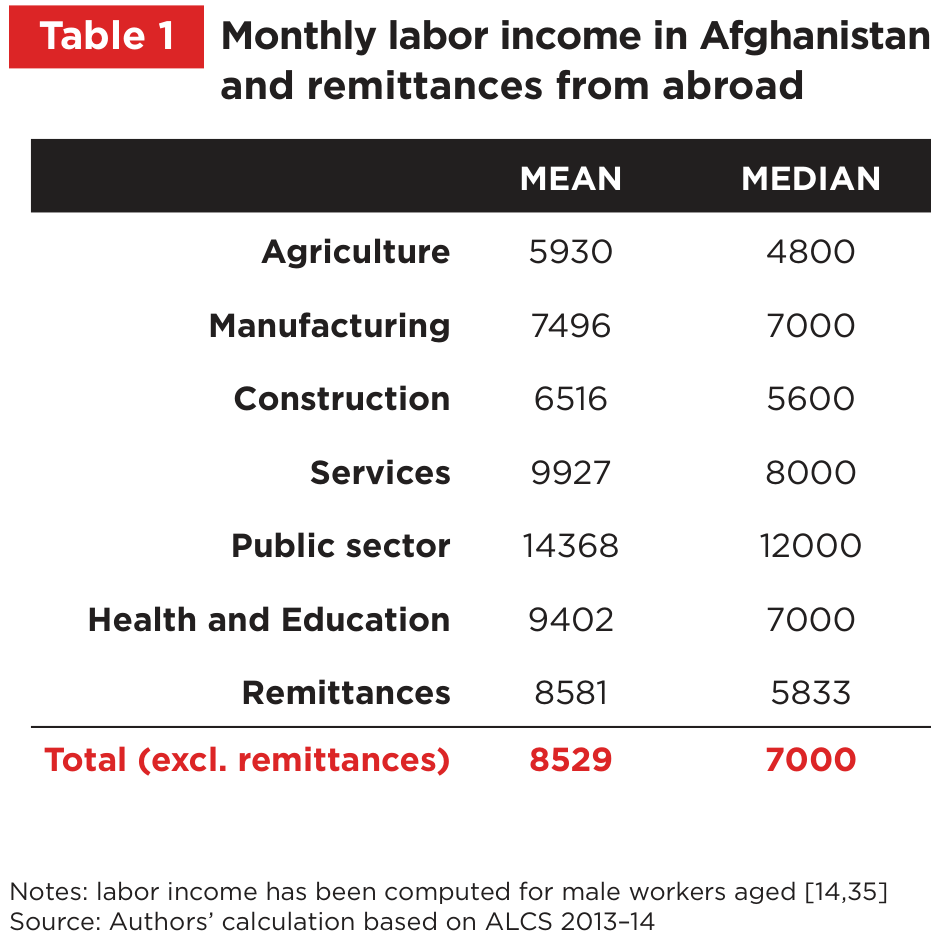
\includegraphics[width=0.55\textwidth]{data/snapshots/108733-revised-public-wb-unhcr-policy-brief-final_table_000.png}

    \vspace{0.5em}
    \scriptsize
    \setlength{\tabcolsep}{3pt}
    \renewcommand{\arraystretch}{0.88}
    \begin{tabularx}{\textwidth}{@{}>{\RaggedRight\arraybackslash}p{0.20\textwidth} >{\RaggedRight\arraybackslash}p{0.23\textwidth} >{\RaggedRight\arraybackslash}X@{}}
        \toprule
        \textbf{Module} & \textbf{Field} & \textbf{Extracted metadata} \\
        \midrule
        Identity \& Discovery & \path{title} & Table 1 Monthly labor income in Afghanistan and remittances from abroad \\
        & \path{document_label} & Table 1 \\
        & \path{subject_domains} & Labor Economics; Remittances \\
        & \path{subject_summary} & Mean and median monthly labor income across employment sectors and remittances for male workers aged 14--35 in Afghanistan \\
        & \path{panel_titles} & \textit{null} \\
        \midrule
        Subject \& Semantics & \path{variable_names} & Monthly labor income; remittances from abroad \\
        & \path{category_dimensions} & Employment sector or income source; summary statistic \\
        & \path{category_labels} & Agriculture; Manufacturing; Construction; Services; Public sector; Health and Education; Remittances; Total excluding remittances; Mean; Median \\
        & \path{population_group} & Male workers aged 14--35 in Afghanistan \\
        \midrule
        Temporal Context & \path{time_period} & 2013--14 \\
        & \path{temporal_granularity} & Monthly \\
        \midrule
        Spatial Context & \path{geographic_scope} & Afghanistan \\
        & \path{geographic_entities} & Afghanistan \\
        & \path{geographic_level} & Country \\
        & \path{geographic_roles} & \textit{null} \\
        & \path{location_types} & \textit{null} \\
        \midrule
        Measurement Context & \path{units_of_measure} & \textit{null} \\
        & \path{currencies} & \textit{null} \\
        & \path{statistical_forms} & Mean; Median \\
        & \path{comparisons} & \textit{null} \\
        \midrule
        Structural Organization & \path{row_dimensions} & Employment sector or income source \\
        & \path{column_dimensions} & Summary statistic \\
        & \path{visualization_types} & Table \\
        \midrule
        Provenance \& Attribution & \path{data_sources} & ALCS 2013--14 \\
        & \path{attributions} & Authors' calculation \\
        & \path{source_document_title} & Fragility and Population Movement in Afghanistan \\
        & \path{languages} & English \\
        & \path{interpretive_notes} & Notes: labor income has been computed for male workers aged [14,35]. \\
        \midrule
        Project \& Operational Context & \path{project_name} & \textit{null} \\
        & \path{project_identifiers} & \textit{null} \\
        & \path{project_components} & \textit{null} \\
        & \path{intervention_types} & \textit{null} \\
        & \path{financing_measures} & \textit{null} \\
        & \path{funders} & \textit{null} \\
        & \path{financing_instruments} & \textit{null} \\
        \midrule
        Analytical \& Methodological Context & \path{analysis_methods} & \textit{null} \\
        & \path{data_collection_methods} & \textit{null} \\
        \bottomrule
    \end{tabularx}
    \caption{A statistical table and its metadata represented using the Data Snapshot Metadata Schema.}
    \label{fig:appendix_extraction_table}
\end{figure}

\clearpage

\subsection{Geospatial visualization}

\begin{figure}[H]
    \centering
    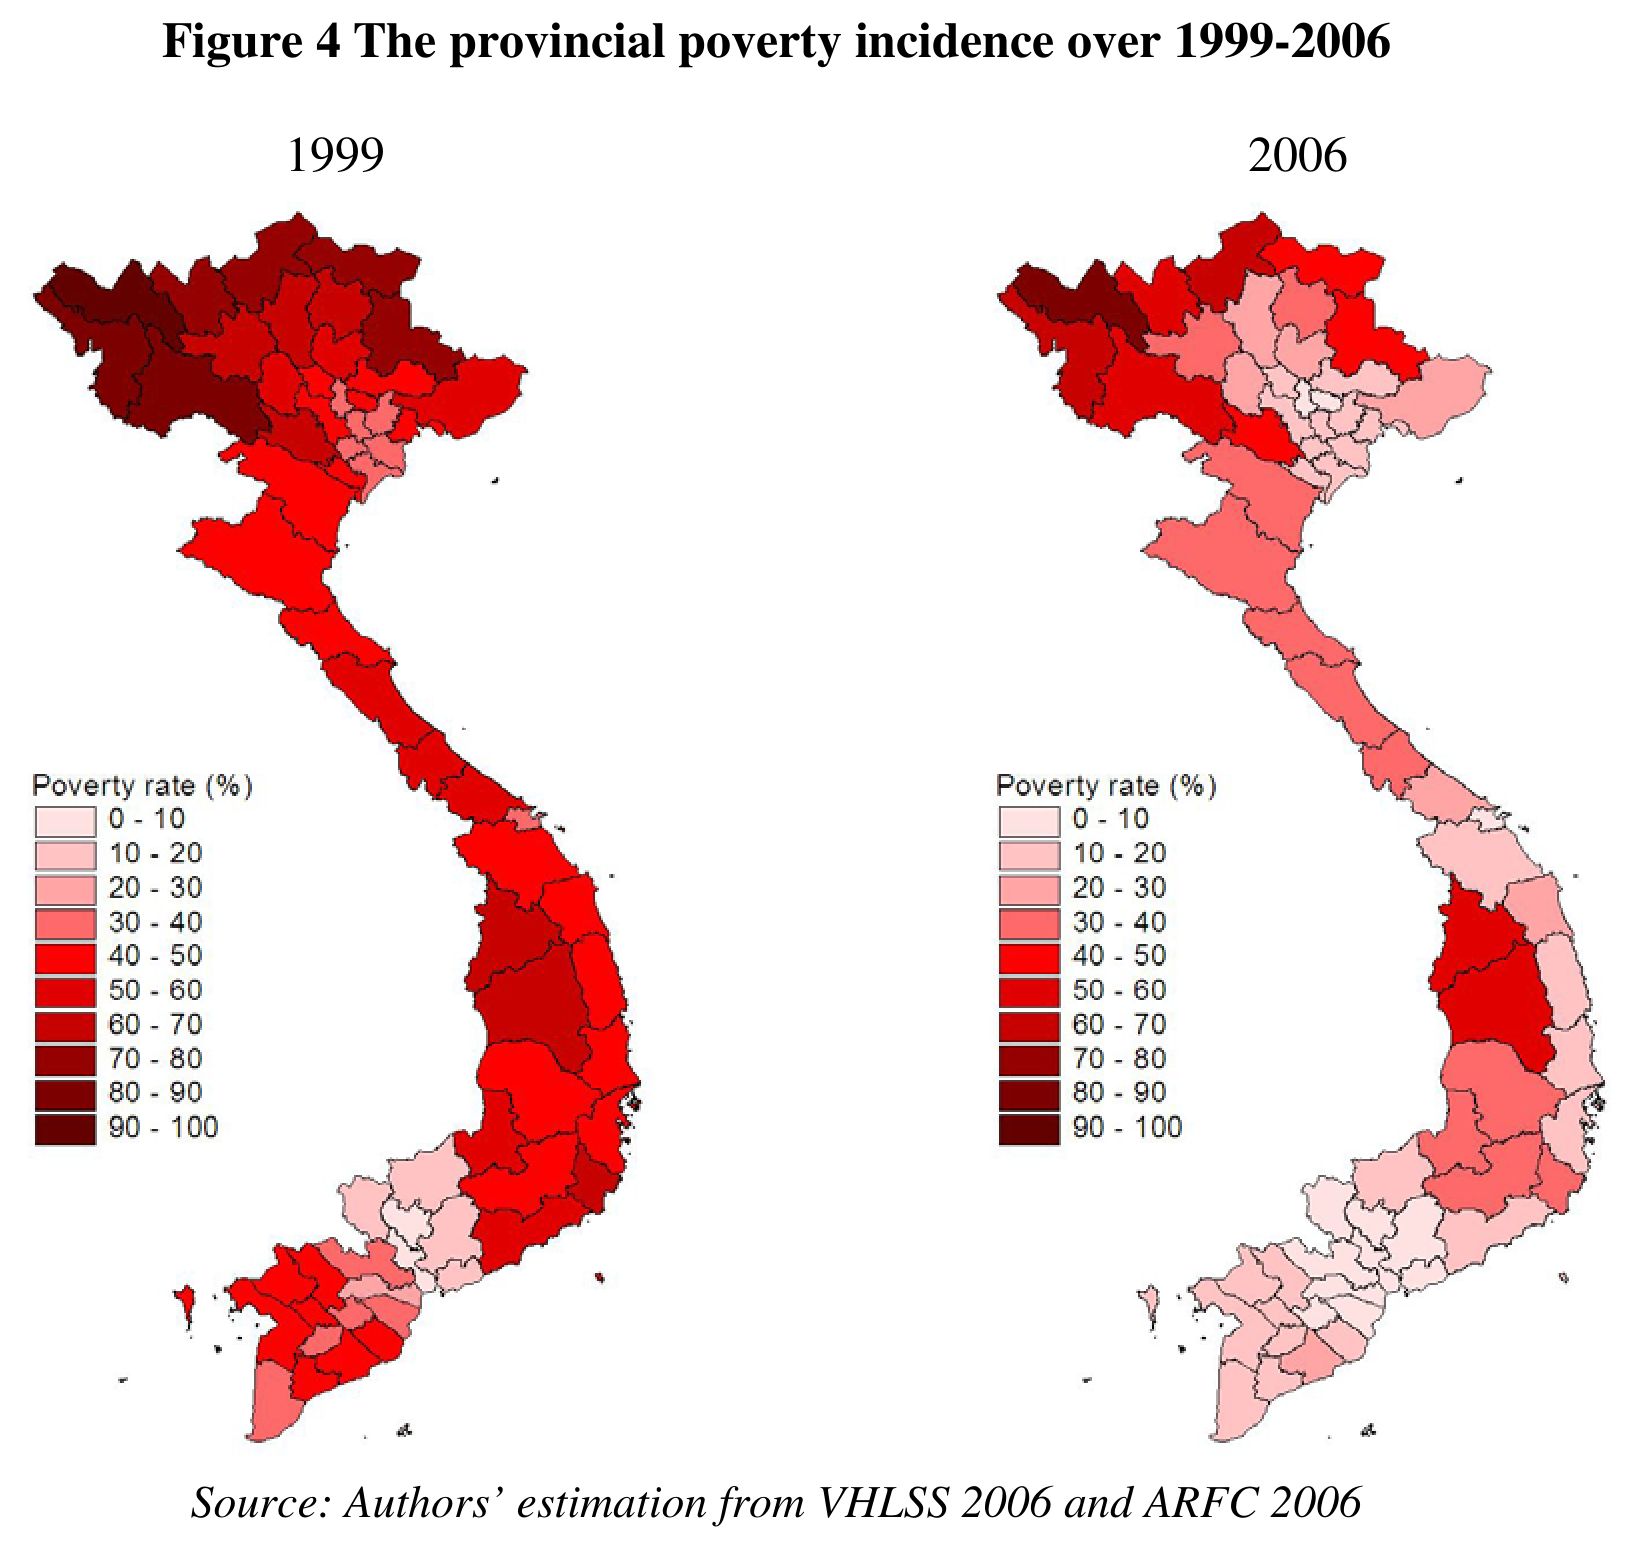
\includegraphics[width=0.55\textwidth]{data/snapshots/document_13148967_figure_003.png}

    \vspace{0.5em}
    \scriptsize
    \setlength{\tabcolsep}{3pt}
    \renewcommand{\arraystretch}{0.88}
    \begin{tabularx}{\textwidth}{@{}>{\RaggedRight\arraybackslash}p{0.20\textwidth} >{\RaggedRight\arraybackslash}p{0.23\textwidth} >{\RaggedRight\arraybackslash}X@{}}
        \toprule
        \textbf{Module} & \textbf{Field} & \textbf{Extracted metadata} \\
        \midrule
        Identity \& Discovery & \path{title} & Figure 4 The provincial poverty incidence over 1999--2006 \\
        & \path{document_label} & Figure 4 \\
        & \path{subject_domains} & Poverty and inequality \\
        & \path{subject_summary} & Provincial poverty incidence in rural Vietnam, comparing 1999 and 2006 \\
        & \path{panel_titles} & 1999; 2006 \\
        \midrule
        Subject \& Semantics & \path{variable_names} & Poverty rate \\
        & \path{category_dimensions} & Poverty rate interval \\
        & \path{category_labels} & 0--10; 10--20; 20--30; 30--40; 40--50; 50--60; 60--70; 70--80; 80--90; 90--100 \\
        & \path{population_group} & Rural population \\
        \midrule
        Temporal Context & \path{time_period} & 1999; 2006 \\
        & \path{temporal_granularity} & \textit{Annual} \\
        \midrule
        Spatial Context & \path{geographic_scope} & Vietnam \\
        & \path{geographic_entities} & \textit{null} \\
        & \path{geographic_level} & Province \\
        & \path{geographic_roles} & \textit{null} \\
        & \path{location_types} & \textit{null} \\
        \midrule
        Measurement Context & \path{units_of_measure} & Percentage \\
        & \path{currencies} & \textit{null} \\
        & \path{statistical_forms} & Rate \\
        & \path{comparisons} & 1999 vs 2006 \\
        \midrule
        Structural Organization & \path{row_dimensions} & \textit{null} \\
        & \path{column_dimensions} & \textit{null} \\
        & \path{visualization_types} & Side-by-side choropleth maps \\
        \midrule
        Provenance \& Attribution & \path{data_sources} & VHLSS 2006; ARFC 2006 \\
        & \path{attributions} & Authors' estimation \\
        & \path{source_document_title} & Poverty and inequality maps for rural Vietnam: an application of small area estimation \\
        & \path{languages} & English \\
        & \path{interpretive_notes} & \textit{null} \\
        \midrule
        Project \& Operational Context & \path{project_name} & \textit{null} \\
        & \path{project_identifiers} & \textit{null} \\
        & \path{project_components} & \textit{null} \\
        & \path{intervention_types} & \textit{null} \\
        & \path{financing_measures} & \textit{null} \\
        & \path{funders} & \textit{null} \\
        & \path{financing_instruments} & \textit{null} \\
        \midrule
        Analytical \& Methodological Context & \path{analysis_methods} & \textit{null} \\
        & \path{data_collection_methods} & \textit{null} \\
        \bottomrule
    \end{tabularx}
    \caption{A geospatial visualization and its metadata represented using the Data Snapshot Metadata Schema.}
    \label{fig:appendix_extraction_map}
\end{figure}

\clearpage

\subsection{Multi-panel chart}

\begin{figure}[H]
    \centering
    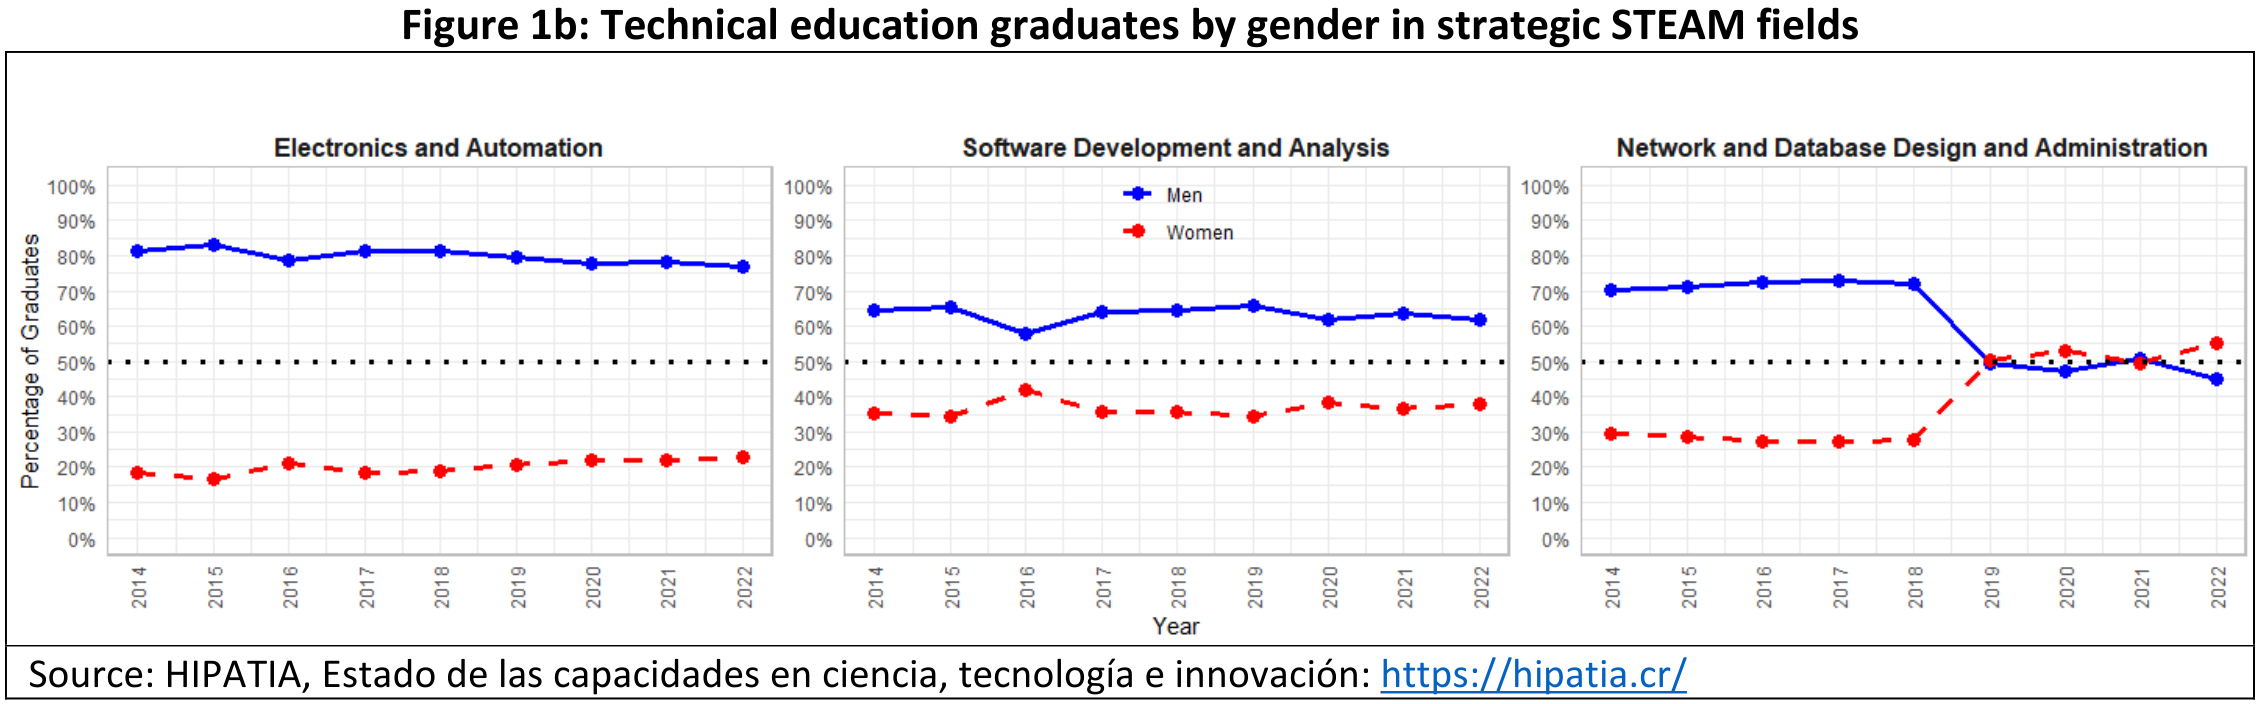
\includegraphics[width=0.95\textwidth]{data/snapshots/005_BOSIB-8191b179-7209-4faa-b5e0-11783bcd492d_figure_001.png}

    \vspace{0.5em}
    \scriptsize
    \setlength{\tabcolsep}{3pt}
    \renewcommand{\arraystretch}{0.88}
    \begin{tabularx}{\textwidth}{@{}>{\RaggedRight\arraybackslash}p{0.20\textwidth} >{\RaggedRight\arraybackslash}p{0.23\textwidth} >{\RaggedRight\arraybackslash}X@{}}
        \toprule
        \textbf{Module} & \textbf{Field} & \textbf{Extracted metadata} \\
        \midrule
        Identity \& Discovery & \path{title} & Figure 1b: Technical education graduates by gender in strategic STEAM fields \\
        & \path{document_label} & Figure 1b \\
        & \path{subject_domains} & Education \\
        & \path{subject_summary} & Gender distribution of technical education graduates across three strategic STEAM fields \\
        & \path{panel_titles} & Electronics and Automation; Software Development and Analysis; Network and Database Design and Administration \\
        \midrule
        Subject \& Semantics & \path{variable_names} & Percentage of graduates \\
        & \path{category_dimensions} & Gender; strategic STEAM field \\
        & \path{category_labels} & Men; Women \\
        & \path{population_group} & Technical education graduates \\
        \midrule
        Temporal Context & \path{time_period} & 2014--2022 \\
        & \path{temporal_granularity} & Annual \\
        \midrule
        Spatial Context & \path{geographic_scope} & \textit{null} \\
        & \path{geographic_entities} & \textit{null} \\
        & \path{geographic_level} & \textit{null} \\
        & \path{geographic_roles} & \textit{null} \\
        & \path{location_types} & \textit{null} \\
        \midrule
        Measurement Context & \path{units_of_measure} & Percentage \\
        & \path{currencies} & \textit{null} \\
        & \path{statistical_forms} & Percentage \\
        & \path{comparisons} & Men vs Women \\
        \midrule
        Structural Organization & \path{row_dimensions} & \textit{null} \\
        & \path{column_dimensions} & \textit{null} \\
        & \path{visualization_types} & Multi-panel line chart \\
        \midrule
        Provenance \& Attribution & \path{data_sources} & HIPATIA, Estado de las capacidades en ciencia, tecnolog\'ia e innovaci\'on \\
        & \path{attributions} & \textit{null} \\
        & \path{source_document_title} & Costa Rica -- Results in Education (CORE) Project \\
        & \path{languages} & English; Spanish \\
        & \path{interpretive_notes} & \textit{null} \\
        \midrule
        Project \& Operational Context & \path{project_name} & \textit{null} \\
        & \path{project_identifiers} & \textit{null} \\
        & \path{project_components} & \textit{null} \\
        & \path{intervention_types} & \textit{null} \\
        & \path{financing_measures} & \textit{null} \\
        & \path{funders} & \textit{null} \\
        & \path{financing_instruments} & \textit{null} \\
        \midrule
        Analytical \& Methodological Context & \path{analysis_methods} & \textit{null} \\
        & \path{data_collection_methods} & \textit{null} \\
        \bottomrule
    \end{tabularx}
    \caption{A multi-panel statistical chart and its metadata represented using the Data Snapshot Metadata Schema.}
    \label{fig:appendix_extraction_chart}
\end{figure}

\clearpage

\section{Appendix: Post-study comparison of schema-validation outputs}
\label{appendix:post_study_validation_comparison}

This appendix reports a follow-on diagnostic conducted after the schema-development study described in the main paper. The diagnostic is included to document an observed change in LLM screening behavior when a later machine-readable schema implementation was evaluated. It is outside the evidentiary boundary of the reported case study: it does not change the paper's schema endpoint, the results of Schema Validations 1 and 2, or the conclusions drawn from those exercises.

Schema Validation 2 evaluated the validated flat Markdown schema before standards-informed refinement. Schema Validation 3 applied the same assessment to a later machine-readable implementation, using its generated JSON Schema as the model-facing representation. In that implementation, Pydantic models served as the canonical source for the JSON Schema and human-readable documentation. The machine-readable implementation also differed structurally from the flat Markdown schema: it organized the fields into nested structures, normalized selected value representations, specified explicit constraints, and encoded relationships among variables, dimensions, provenance, temporal and geographic coverage, projects, and financing.

\subsection{Comparison design and claim boundary}

Both exercises used the same 202 snapshots, associated parent-document metadata, one-snapshot-per-request design, GPT-5.5 model configuration, and materiality-focused candidate threshold. The response contract remained substantively equivalent, but Schema Validation 3 replaced references to the closest flat fields with exact nested schema paths. Table~\ref{tab:validation2_validation3_design} distinguishes these retained conditions from the changes introduced in the follow-on exercise.

\begin{table}[H]
    \centering
    \caption{Conditions retained and changed between Schema Validations 2 and 3.}
    \label{tab:validation2_validation3_design}
    \renewcommand{\arraystretch}{1.15}
    \small
    \begin{tabularx}{\textwidth}{>{\RaggedRight\arraybackslash}p{0.23\textwidth} >{\RaggedRight\arraybackslash}X >{\RaggedRight\arraybackslash}X}
        \toprule
        \textbf{Dimension} & \textbf{Schema Validation 2} & \textbf{Schema Validation 3} \\
        \midrule
        Substantive evidence & Same 202 held-out snapshots & Same 202 snapshots \\
        Assessment configuration & GPT-5.5; medium reasoning; Flex; one snapshot per request & Same configuration \\
        Assessment threshold & Critical or possibly critical reusable omission with material impact & Same threshold \\
        Schema content & Validated flat 36-field specification before standards-informed refinement & Nested and normalized machine-readable contract \\
        Canonical representation & Markdown specification & Pydantic models \\
        Model-facing representation & History-neutral flat Markdown schema & Generated JSON Schema \\
        Candidate references & Closest flat schema fields & Exact nested schema paths \\
        \bottomrule
    \end{tabularx}
\end{table}

These changes prevent causal attribution. The comparison cannot determine whether differences in model output arose from schema content, Markdown versus JSON Schema, the amount and explicitness of schema context, path-based reporting, or nondeterministic model behavior. Schema Validation 3 is therefore treated as a repeated assessment under the later machine-readable schema implementation, not as an experiment isolating a representation-format effect.

\subsection{Observed screening results}

The raw screening outputs differed substantially (Table~\ref{tab:validation2_validation3_results}). Schema Validation 2 produced six candidate records across five positive snapshots. Schema Validation 3 produced 36 candidate records across 31 positive snapshots. Its 202 calls used approximately 2.2 times as many input tokens because the generated JSON Schema supplied a larger and more explicit contract.

\begin{table}[H]
    \centering
    \caption{Observed model outputs and adjudicated field-level outcomes.}
    \label{tab:validation2_validation3_results}
    \renewcommand{\arraystretch}{1.1}
    \small
    \begin{tabular}{lrr}
        \toprule
        \textbf{Measure} & \textbf{Validation 2} & \textbf{Validation 3} \\
        \midrule
        No-gap snapshots & 197 & 171 \\
        Possible-gap snapshots & 5 & 28 \\
        Critical-gap snapshots & 0 & 3 \\
        Positive snapshots & 5 & 31 \\
        Candidate records & 6 & 36 \\
        Total input tokens & 2,450,382 & 5,396,754 \\
        Total output tokens & 92,709 & 150,326 \\
        Accepted new standalone fields & 0 & 0 \\
        \bottomrule
    \end{tabular}
\end{table}

The paired snapshot-level results also changed. Of the 197 snapshots assessed as having no critical gap in Validation 2, Validation 3 assessed 168 as no-gap, 27 as possible-gap, and two as critical-gap cases. Of the five Validation 2 possible-gap snapshots, Validation 3 assessed three as no-gap, one as possible, and one as critical. In total, 33 of 202 snapshots changed assessment category. These changes describe model screening behavior; they do not by themselves establish schema regressions.

The 36 Validation 3 candidates were concentrated in seven review families (Table~\ref{tab:validation3_candidate_families}). The three largest families accounted for 26 candidates. This concentration shows that the increase was driven primarily by repeated pressure on a small number of structural and scope boundaries rather than by 36 distinct missing metadata subjects.

\begin{table}[H]
    \centering
    \caption{Candidate families produced by Schema Validation 3.}
    \label{tab:validation3_candidate_families}
    \renewcommand{\arraystretch}{1.1}
    \small
    \begin{tabularx}{\textwidth}{>{\RaggedRight\arraybackslash}X r >{\RaggedRight\arraybackslash}p{0.49\textwidth}}
        \toprule
        \textbf{Candidate family} & \textbf{Count} & \textbf{Primary concern} \\
        \midrule
        Cartographic representation & 12 & Map scales and numerical coordinate extents \\
        Hierarchy and internal structure & 7 & Deeper table hierarchies, conditional structures, and diagram flows \\
        Scoped metadata associations & 7 & Per-variable, per-note, or per-panel association of existing concepts \\
        Value and observation semantics & 5 & Value status, respondent groups, observational units, and collection responsibility \\
        Visual-axis encoding & 3 & Distinct axes, truncated marks, and nonzero axis ranges \\
        Cross-snapshot relationships & 1 & Reference to a related snapshot \\
        Source-visible label representation & 1 & Icon-only column labels \\
        \midrule
        \textbf{Total} & \textbf{36} & \\
        \bottomrule
    \end{tabularx}
\end{table}

Human adjudication produced a substantially narrower result (Table~\ref{tab:validation3_adjudication}). Thirteen candidates concerned extraction or internal visual structure, and eleven lacked sufficient evidence, generalizability, or materiality. Seven were already represented adequately by the machine-readable schema. No candidate was accepted as a new standalone metadata field.

\begin{table}[H]
    \centering
    \caption{Human dispositions for the 36 Schema Validation 3 candidates.}
    \label{tab:validation3_adjudication}
    \renewcommand{\arraystretch}{1.1}
    \small
    \begin{tabularx}{0.82\textwidth}{>{\RaggedRight\arraybackslash}X r}
        \toprule
        \textbf{Human disposition} & \textbf{Candidates} \\
        \midrule
        Covered adequately by the machine-readable schema & 7 \\
        Extraction or internal visual structure & 13 \\
        Insufficient evidence, generalizability, or materiality & 11 \\
        Outside the snapshot-metadata boundary & 1 \\
        Documentation or representation concern & 3 \\
        Meaningful representation gap & 1 \\
        \midrule
        \textbf{Total} & \textbf{36} \\
        \bottomrule
    \end{tabularx}
\end{table}

The one accepted representation gap concerned a multi-axis graph. The machine-readable schema evaluated in Validation 3 could identify a general axis role but could not associate each variable with the distinct axis required to interpret it. This finding concerned a relationship among existing concepts rather than a missing metadata subject and was addressed after the run through a bounded structural refinement of the variable representation. Two panel-association candidates reproduced the concern already identified in Validation 2. Proposals for deeper recursive hierarchies did not overturn the nonrecursive grouping boundary adopted in the machine-readable schema.

\subsection{Interpretation of the divergence}

Several features of the later instrument plausibly contributed to the larger review set. First, the machine-readable contract made structural ownership and constraints explicit. A model could therefore identify that a concept existed while questioning whether it could be attached to a particular variable, panel, note, or category. Second, the generated JSON Schema provided substantially more input context than the flat Markdown schema. This increased the number of explicit structures and boundaries against which each snapshot could be compared. Third, exact nested-path reporting encouraged candidates to be localized to relationship and cardinality boundaries rather than expressed only as absent flat fields.

The candidate composition provides additional evidence about the nature of the divergence. Many proposals concerned map calibration, coordinate bounds, recursive table structure, conditional denominators, axis ranges, or diagram flows. These features could support reconstruction of internal snapshot content, but they fall outside the intended role of a snapshot-level metadata schema. The more explicit schema therefore surfaced additional pressure at the boundary between metadata description and visual-content extraction.

These observations remain explanatory hypotheses rather than isolated effects. Individual LLM calls are nondeterministic, and neither exercise repeated the full assessment sufficiently to characterize run-to-run variance. Because schema semantics and model-facing representation changed together, the observed difference cannot establish that JSON Schema is intrinsically more or less suitable than Markdown for LLM-assisted validation.

\subsection{Implications and future evaluation}

The adjudicated outcomes are more consistent than the raw screening counts. Validation 2 and Validation 3 both accepted no new standalone metadata field. The later exercise reproduced one previously identified panel concern, retained the chosen boundary for hierarchical structure, and identified one additional structural association within the existing variable concept. The larger candidate set therefore does not indicate that the later schema omitted more accepted metadata concepts.

The later machine-readable implementation nevertheless indicates a practical direction for schema maintenance. A canonical Pydantic model can make types, nesting, cardinalities, and constraints machine-enforceable while generating JSON Schema and human-readable documentation as derivatives. This avoids maintaining Markdown as an independent authoritative schema while preserving a readable reference for human review. These implementation benefits are separate from the unresolved question of how representation affects LLM assessment behavior.

A causal evaluation would need to vary schema semantics and model-facing presentation independently. One design would present both the schema as described in this paper and the later machine-readable schema in comparable Markdown and JSON Schema forms, repeat each condition across multiple model runs, and apply the same human-adjudication procedure. Such a study could distinguish effects associated with schema content, serialization format, and model variability. The present appendix documents the motivating observation but does not answer that causal question.

\end{document}
